\section{Evaluation} 
\label{sec:Expts}
In this section, we describe the experimental setup for the construction and evaluation of ontological tag trees. For the evaluation, we define tag prediction and efficient classification tasks as discussed later in this section. The experiments are conducted on two large corpora of images, the details of which are given below.  
\vspace{-0.1in}
\subsection{Datasets} 
\label{sec:Datasets}
To test the robustness of our approach to build ontological tag trees for domains with varying degrees of tag noise, we use two different image corpora - one from Flickr, composed primarily of user generated content, and one from a professionally curated stock photo agency.
\begin{itemize} 
\item \textbf{Flickr images}: Flickr~\cite{Flickr} is a popular image and video hosting website where users can upload images and associate them with annotations such as titles, tags and descriptions, among others. As Flickr primarily contains user generated content, tags are often noisy, irrelevant to image content or even completely absent. 
%As can be seen in Fig.~\ref{fig:CDFFlickr}, more than 90\% Flickr images have 13 or less tags associated with them. 
We utilize 500,000 images for training and 100,000 images for testing. All these images are licensed under Creative Commons copyright licenses.
\item \textbf{Stock images corpus}: To evaluate the proposed approach on less noisy data, we take a corpus of stock photos that are professionally annotated, and hence are accompanied with a variety of accurate annotations - such as keywords, captions, etc. For this corpus, we use the set of keywords to build the ontological tag tree, and refer to them as "tags".
%Images are professionally annotated and hence 90\% of Getty images have 38 or less tags (Fig.~\ref{fig:CDFGetty}), which is much more than in the case of Flickr. 
We utilize more than 350,000 images for training and close to 70,000 images for testing. The textual captions are used in the efficient classification task as shown in Section~\ref{sec:effClassification}.
\end{itemize} 

Training images are used for adapting the WordNet based preliminary tag tree obtained using Algorithm~\ref{alg:WordNetSTAlgo} to the given corpus using the local search based approach described in Algorithm~\ref{algo:STCAlgorithm}. Training images are also used for specific required tasks such as training of classifiers. Testing images are used to evaluate the constructed tag trees. There is no overlap between training and test sets.



\subsection{Effect of Local Search based Optimization}
We first demonstrate how the proposed local search based approach helps in improving the objective function as defined in Section~\ref{sec:ConstructionTree}. Fig.~\ref{fig:ObjFun} shows the variation of the objective function in (\ref{eq:ObjFnWeightedHops}) with the number of iterations on Flickr tag corpus. The objective function value of the WordNet based preliminary tag tree for Flickr corpus before the proposed refinement is $357.2$ that becomes $167.1$ using the local search based refinement in $68$ iterations. Median of the Jaccard similarity values is taken as the threshold $\tau$ for candidate selection in the proposed refinement algorithm. Similar improvement is observed for the Stock images corpus, for which the objective function values improves from $224.5$ to $99$ after 23 iterations. For both corpora, the iterations are terminated once no further improvement is observed in the objective function. We describe below the tasks defined to evaluate the constructed tag trees. 
\begin{figure}[h!]
\begin{center}
%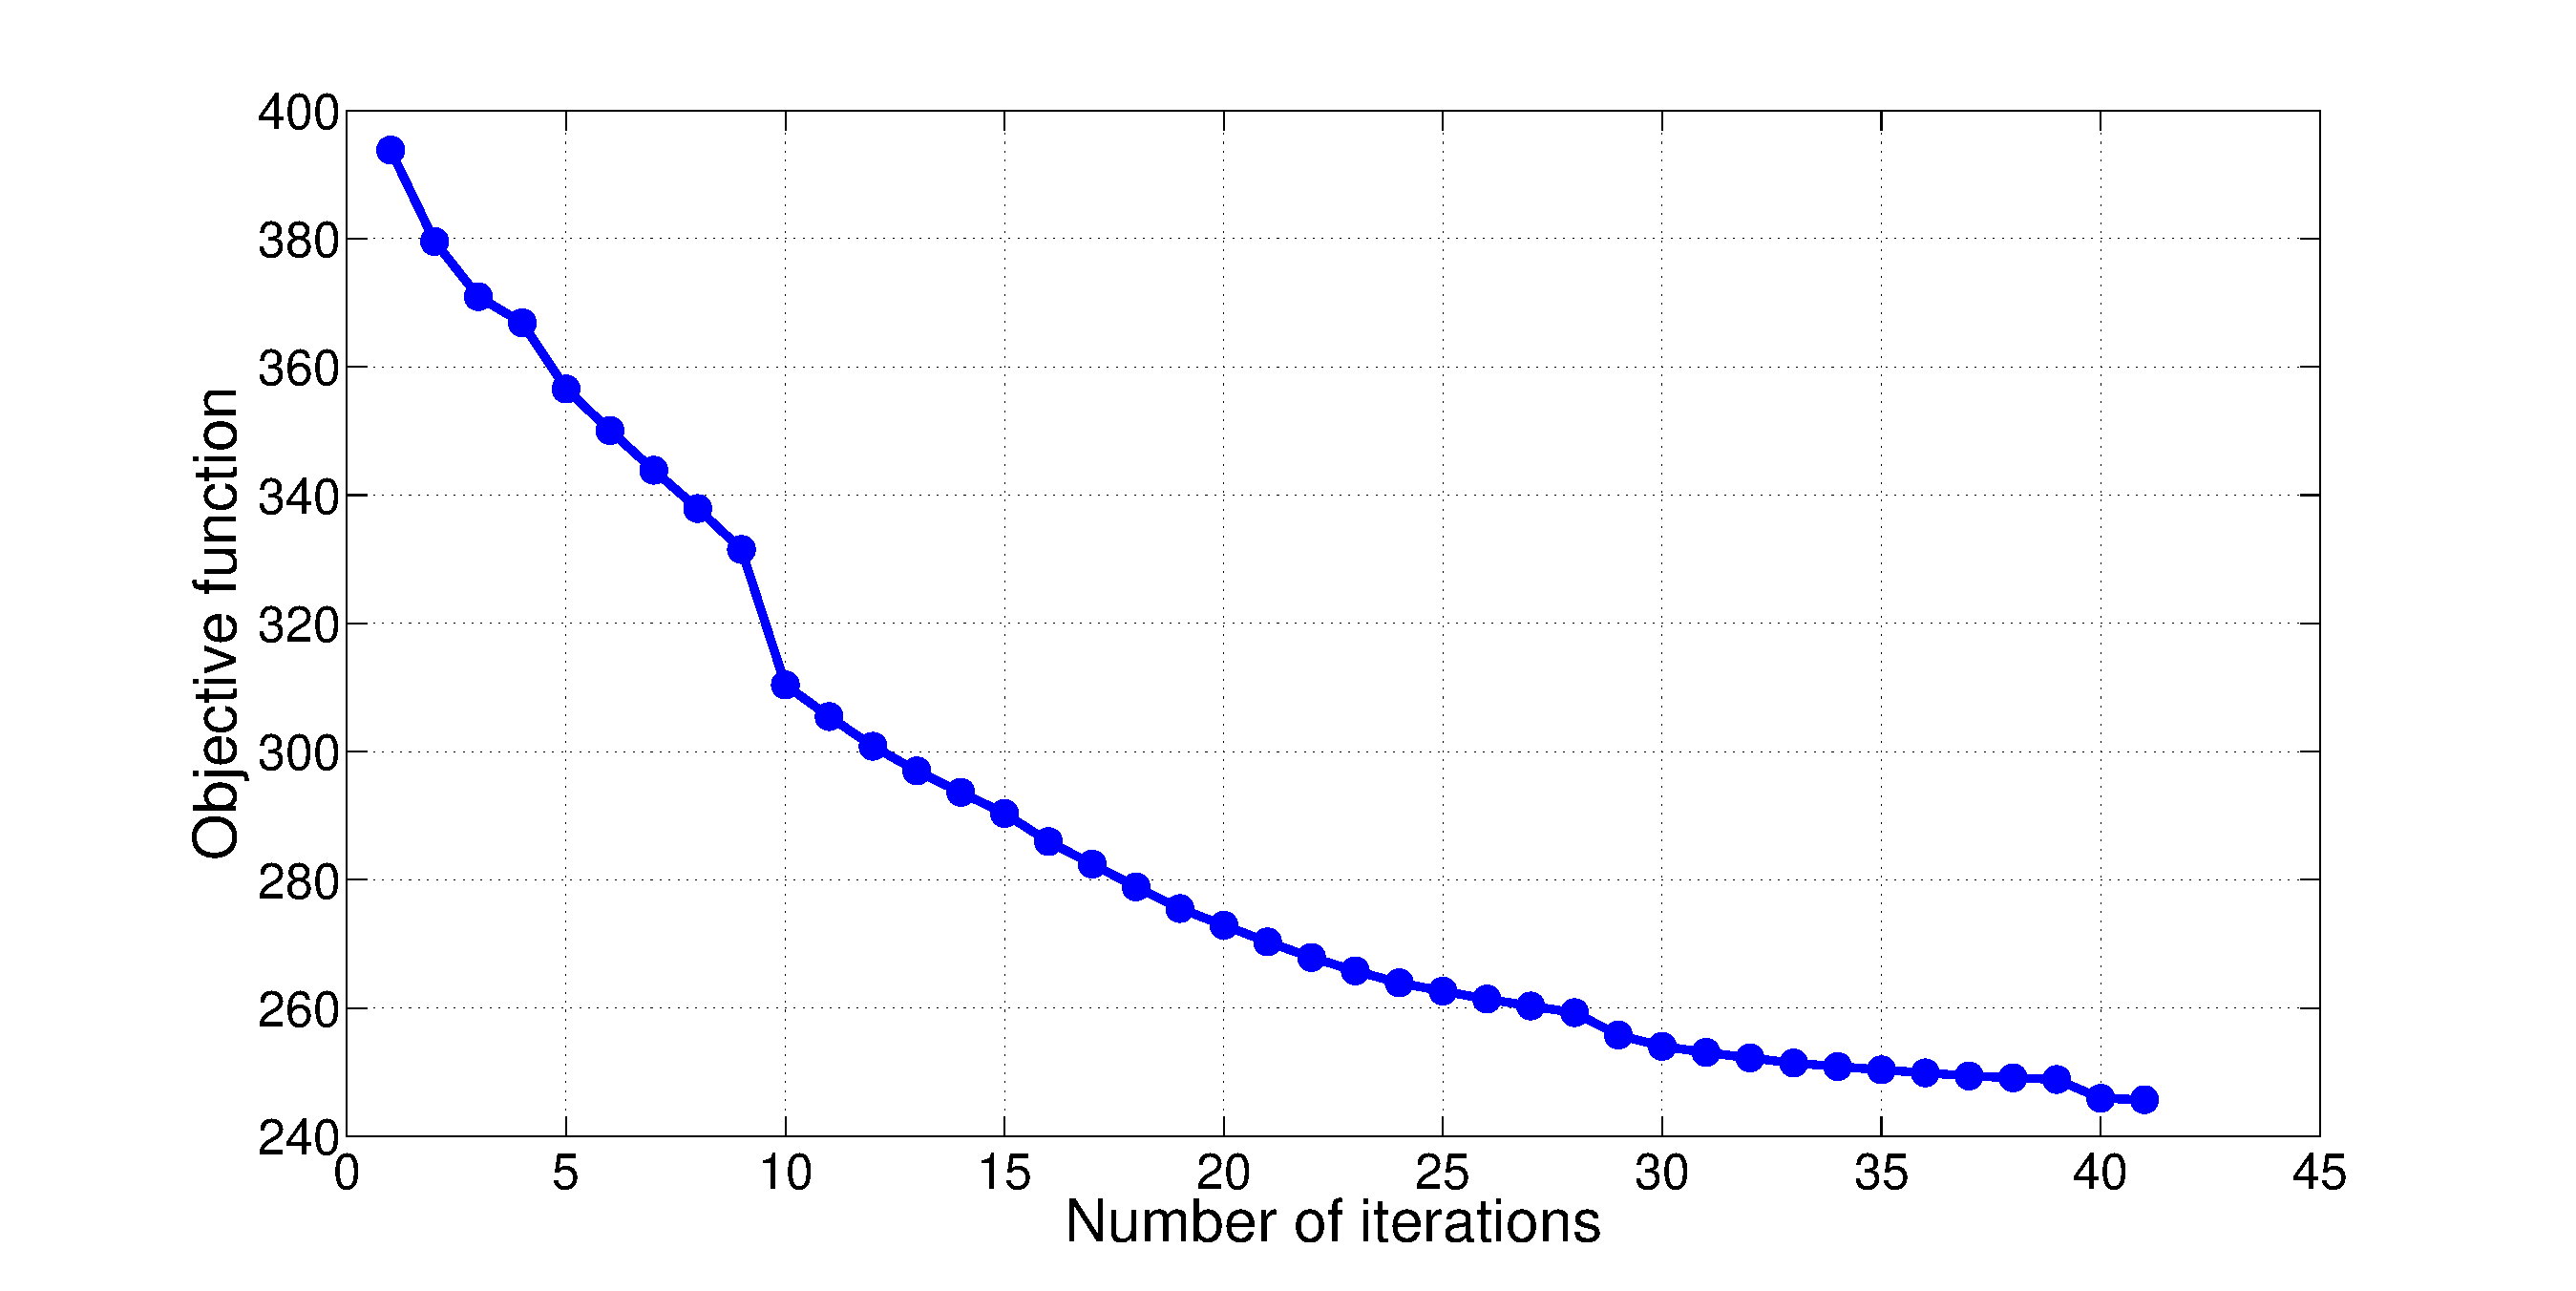
\includegraphics[width=0.8\linewidth]{TagTree/SigmaCijDijVariatPerIter999point05STGD}
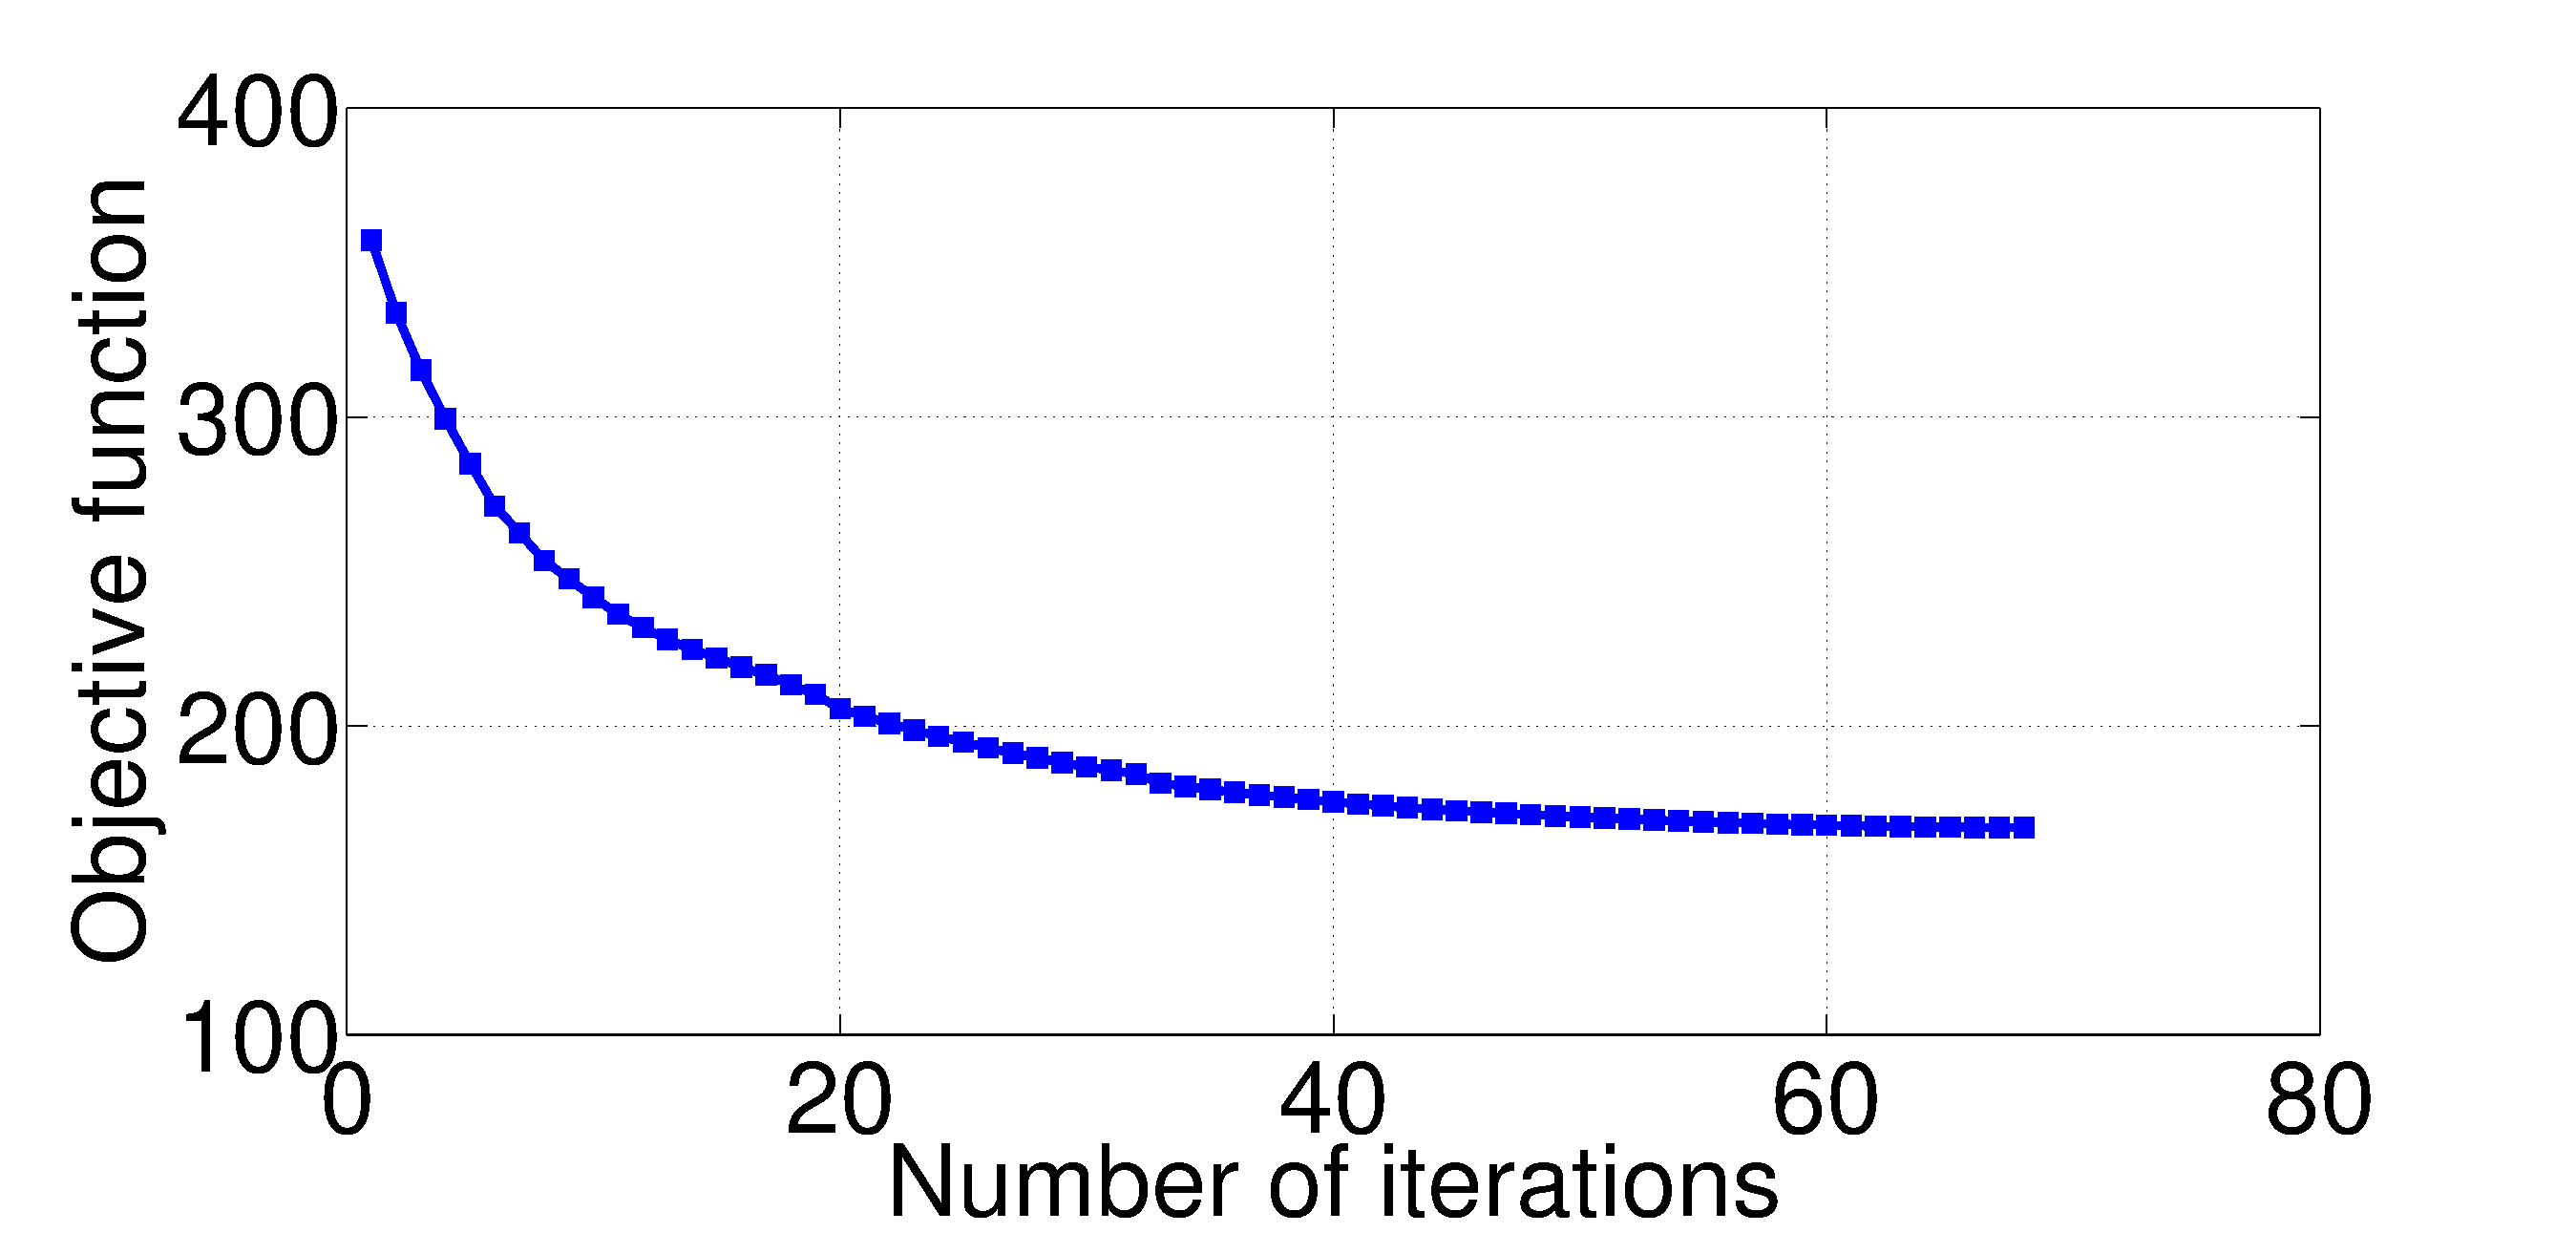
\includegraphics[width=0.65\linewidth]{TagTree/LSWWW_objectivefnValuePerIteration}
\caption{The variation of the objective function~(\ref{eq:ObjFnWeightedHops}) with the number of iterations for a sample run on Flickr tag corpus.} 
\label{fig:ObjFun}
\end{center}
\end{figure}
%We describe below the tasks defined to evaluate the constructed tag trees. 
% \indent \textit{Subsumption-based Semantic Graph} - \cite{SubsumptionText} and \cite{SubsumptionFlickr} utilize a rule-based subsumption model to derive hierarchies from text corpus and Flickr respectively. We utilize the same model to construct hierarchy for keywords of interest, and construct semantic graph by disregarding parent-child relationships and keeping only the edges. \\ 
% \indent We evaluate the performance of a semantic graph by utilizing the graph to assist in classification as detailed below. 
\subsection{Tag Prediction Task} 
\label{subsec:TagPred}
%The intuition behind this task is that a semantic graph that provides better performance in tag prediction is able to capture the information that characterizing the corpus in a much better manner. 
%Tag prediction is performed with the help of a given graph as detailed below. 
 
\hl{The tag prediction task is similar to the tag recommendation task in  {\cite{katsurai2013cross}} and in {\cite{sigurbjornsson2008flickr}}. However as outlined in Section {\ref{sub_sec:relatedWork}}, the proposed task does not require manual labeling for the resources (images) to evaluate the proposed tag tree construction approach. In order to do so, we divide the tags associated with a resource into a seen and an an unseen set of tags and use the latter to evaluate the predicted tags. We demonstrate this approach through experiments conducted on image corpora. 
}
Let an image $i$ in the corpus be tagged with the set of tags $\mathcal{T}_i$, such that $\mid \mathcal{T}_i \mid =N_{Tags}$. Assume that out of these $N_{Tags}$ tags, only a subset $\mathcal{T}_{i,Seen}$ are observed, with $\mid \mathcal{T}_{i,Seen} \mid=N_{Seen}$. The objective of the \emph{tag prediction task} is to predict the remaining ($N_{Tags} - N_{Seen}$) tags, i.e., $\mathcal{T}_i \setminus \mathcal{T}_{i,Seen}$.  Let $\mathbb{P}_i$ be the set of ($N_{Tags} - N_{Seen}$) tags predicted for image $i$ assuming that $\mathcal{T}_{i,Seen}$ is observed. Note that the prediction assumes the total number of tags for the image, $N_{Tags}$, to be known. Performance of tag prediction can be measured by the \emph{Tag Prediction Accuracy}, defined as follows: 
\begin{equation} \label{eq:TagPredAccuracy}
%\text{Tag Prediction Score} = \frac{\mid  \{\mathcal{T}_i \setminus  \mathcal{T}_{i,Seen}\} \cap \mathbb{P}_i \mid}{ \mid \{  \mathcal{T}_i \setminus  \mathcal{T}_{i,Seen} \}  \cup \mathbb{P}_i \mid} .
\text{Tag Prediction Accuracy} = \frac{\mid  \{\mathcal{T}_i \setminus  \mathcal{T}_{i,Seen}\} \cap \mathbb{P}_i \mid}{ \mid \{  \mathcal{T}_i \setminus  \mathcal{T}_{i,Seen} \} \mid} .
\end{equation} 

We now discuss the approach we follow to obtain the set of predicted tags $\mathbb{P}_i$ when the set of tags $\mathcal{T}_{i,Seen}$ is seen, by utilizing a given ontological tag tree. 
\subsubsection{Utilizing Ontological Tag Tree for Tag Prediction} 
\label{sec:TagPredUsingGraph}
Consider the tag tree $T$, built over the set of $\mathcal{T}$ tags in a corpus. For image $i$ with $N_{Seen}$ number of seen tags, each tag $t \in \{ \mathcal{T} \setminus \mathcal{T}_{i,Seen} \}$ is given a proximity score $s_t$ based on its proximity from the seen tags, as per $T$. Specifically, 
\begin{equation} 
s_t = \Sigma_{t' \in \mathcal{T}_{i,Seen} }{dist(t,t')}, 
\label{eq:TPEquation}
\end{equation}
where $dist(t,t')$ is the distance between tags $t$ and $t'$ in $T$ calculated as shown in Section~\ref{sec:comparison}. A lower proximity score for a tag $t$ indicates that it is closer in a cumulative sense to the set of observed tags $\mathcal{T}_{i,Seen}$. The tags are ordered in the increasing order of $s_t$, and the first ($N_{Tags} - N_{Seen}$) tags, i.e. those corresponding to the least values of $s_t$, are chosen as the set of predicted tags $\mathbb{P}_i$. \\

\subsubsection{Methods Compared} 
\label{sec:comparison}
We compare the following methods in the tag prediction task:
\begin{enumerate}
\item \underline{Random}: As the name suggests, this baseline method randomly picks  ($N_{Tags} - N_{Seen}$)  tags from the set $\mathcal{T} \setminus \mathcal{T}_{i,Seen}$. 

\item \underline{WordNet}: This baseline approach uses the semantics based ontological tag tree constructed from WordNet hierarchy using the procedure described in Algorithm 1. The edge weights are assigned to be semantic distances as obtained from \cite{RitaLibraryWordNet}. 
%\item \underline{(Weighted) WordNet hierarchy}: Same as the previous approach with the only difference being that semantic WordNet distances are used as edge weights instead of assigning them to $1$.
\item \underline{Google Similarity Distance}:  Google Similarity Distance \cite{cilibrasi2007google} has been used to construct tag graphs in applications such as tag ranking \cite{liu2009tag}. As mentioned in Section~\ref{sub_sec:relatedWork}, a threshold is used to discard certain edges in tag graphs. We choose a threshold such that for a tag graph with $N$ nodes (or tags), there are exactly $(N-1)$ edges remaining, so that the tag graph thus formed has same number of edges and space requirement as the tag tree learnt from proposed approach. Edge weights for the tag graph are taken to be the Google Similarity Distance as defined in \cite{cilibrasi2007google}. 

%In the approach, we obtain the tag graph based on the Google Distance model~\cite{SubsumptionFlickr}. In order to compare against the proposed approach, this is converted to an ontological graph by ignoring the directions and connecting the node with highest degree in each disconnected components, to a ``Root" node. The resulting subsumption graph is a spanning tree over the set of tags and an additional ``Root" node. 

\item \underline{LS Weighted Average Hops (LS-WAH)}:  Here we construct a tag tree using the proposed local search based approach, to minimize Weighted Average Hops (\ref{eq:ObjFnWeightedHops}) in Section~\ref{sec:refinement}. If an edge exists between tags $t_i$ and $t_j$ then the weight of the edge connecting them is given to be $(1-J_{\mathcal{T}}(i,j))$. 

\item \underline{LS Similarity Approximation (LS-SA)}:  This tag tree is constructed using the proposed approach with objective corresponding to Similarity Approximation as outlined in (\ref{eq:ObjFnSimApprox}) in Section~\ref{sec:refinement}. The edge weights are assigned as in Method 4 above. 

\item \underline{Symmetric sum based}: \hl{In order to compare the performance of the proposed tag tree construction approaches with that of other tag recommendation approaches that do not use tag trees or tag graphs or any visual features, we also provide the performance of the symmetric sum based approach as proposed in {\cite{sigurbjornsson2008flickr}}. Note that the space required to store the pair-wise similarities in {\cite{sigurbjornsson2008flickr}} is $O(N^2)$ while the proposed tag tree construction requires $O(N)$ space to store the tag tree. 
}


%For all present edges in the constructed tree, the weight of the edge is taken to be the jaccard similarity of the connecting tags. 

%\item \underline{LS on WordNet hierarchy}: This approach uses the refined ontological graph obtained using the proposed local search based algorithm (Algorithm 2). The edge weights are assigned to $1$ in this variant of the approach. 

%\item \underline{(Weighted) LS on WordNet hierarchy}: Same as the previous approach with the only difference being that inverse of Jaccard similarities are used as edge weights instead of assigning them to $1$.

\end{enumerate}
The prediction task is performed using the approach described in section~\ref{sec:TagPredUsingGraph}. For methods numbered 2, 3, and 4 above, $dist(t_i, t_j)$ as required in $(\ref{eq:TPEquation})$ is calculated by adding distances of edges in path connecting tags $t_i$ and $t_j$. For LS-SA method, $dist(t_i, t_j)$ is defined as $\{1- S_T{(i,j)}    \}$ where $S_T{(i,j)}$ is calculated for an ontological tag tree $T$ as per $(\ref{eq:ProdSimSimilarityCalculate})$. This is because the tag tree construction approach for LS-SA method utilizes product based similarity approximation $(\ref{eq:ProdSimSimilarityCalculate})$ and so it is appropriate to use same approach to estimate similarities based on a tree, and hence to calculate $dist(t_i, t_j)$. \hl{Similarly, for Symmetric sum based method {\cite{sigurbjornsson2008flickr}}, $dist(t_i, t_j)$ is defined as $\{1- J_{\mathcal{T}}(i,j)    \}$ where $J_{\mathcal{T}}(i,j)$ is the jaccard similarity between tag $t_i$ and $t_j$ as defined in Section~{\ref{sec:refinement}}. Note that this makes ({\ref{eq:TPEquation}}) similar to the sum based scoring approach in {\cite{sigurbjornsson2008flickr}}. 
}

%\indent The tag prediction task is conducted on two corpora, Flickr and the stock images corpus. We present the results in detail below. \\
\comment{
\begin{figure*}[!ht]
\minipage{0.32\textwidth}
  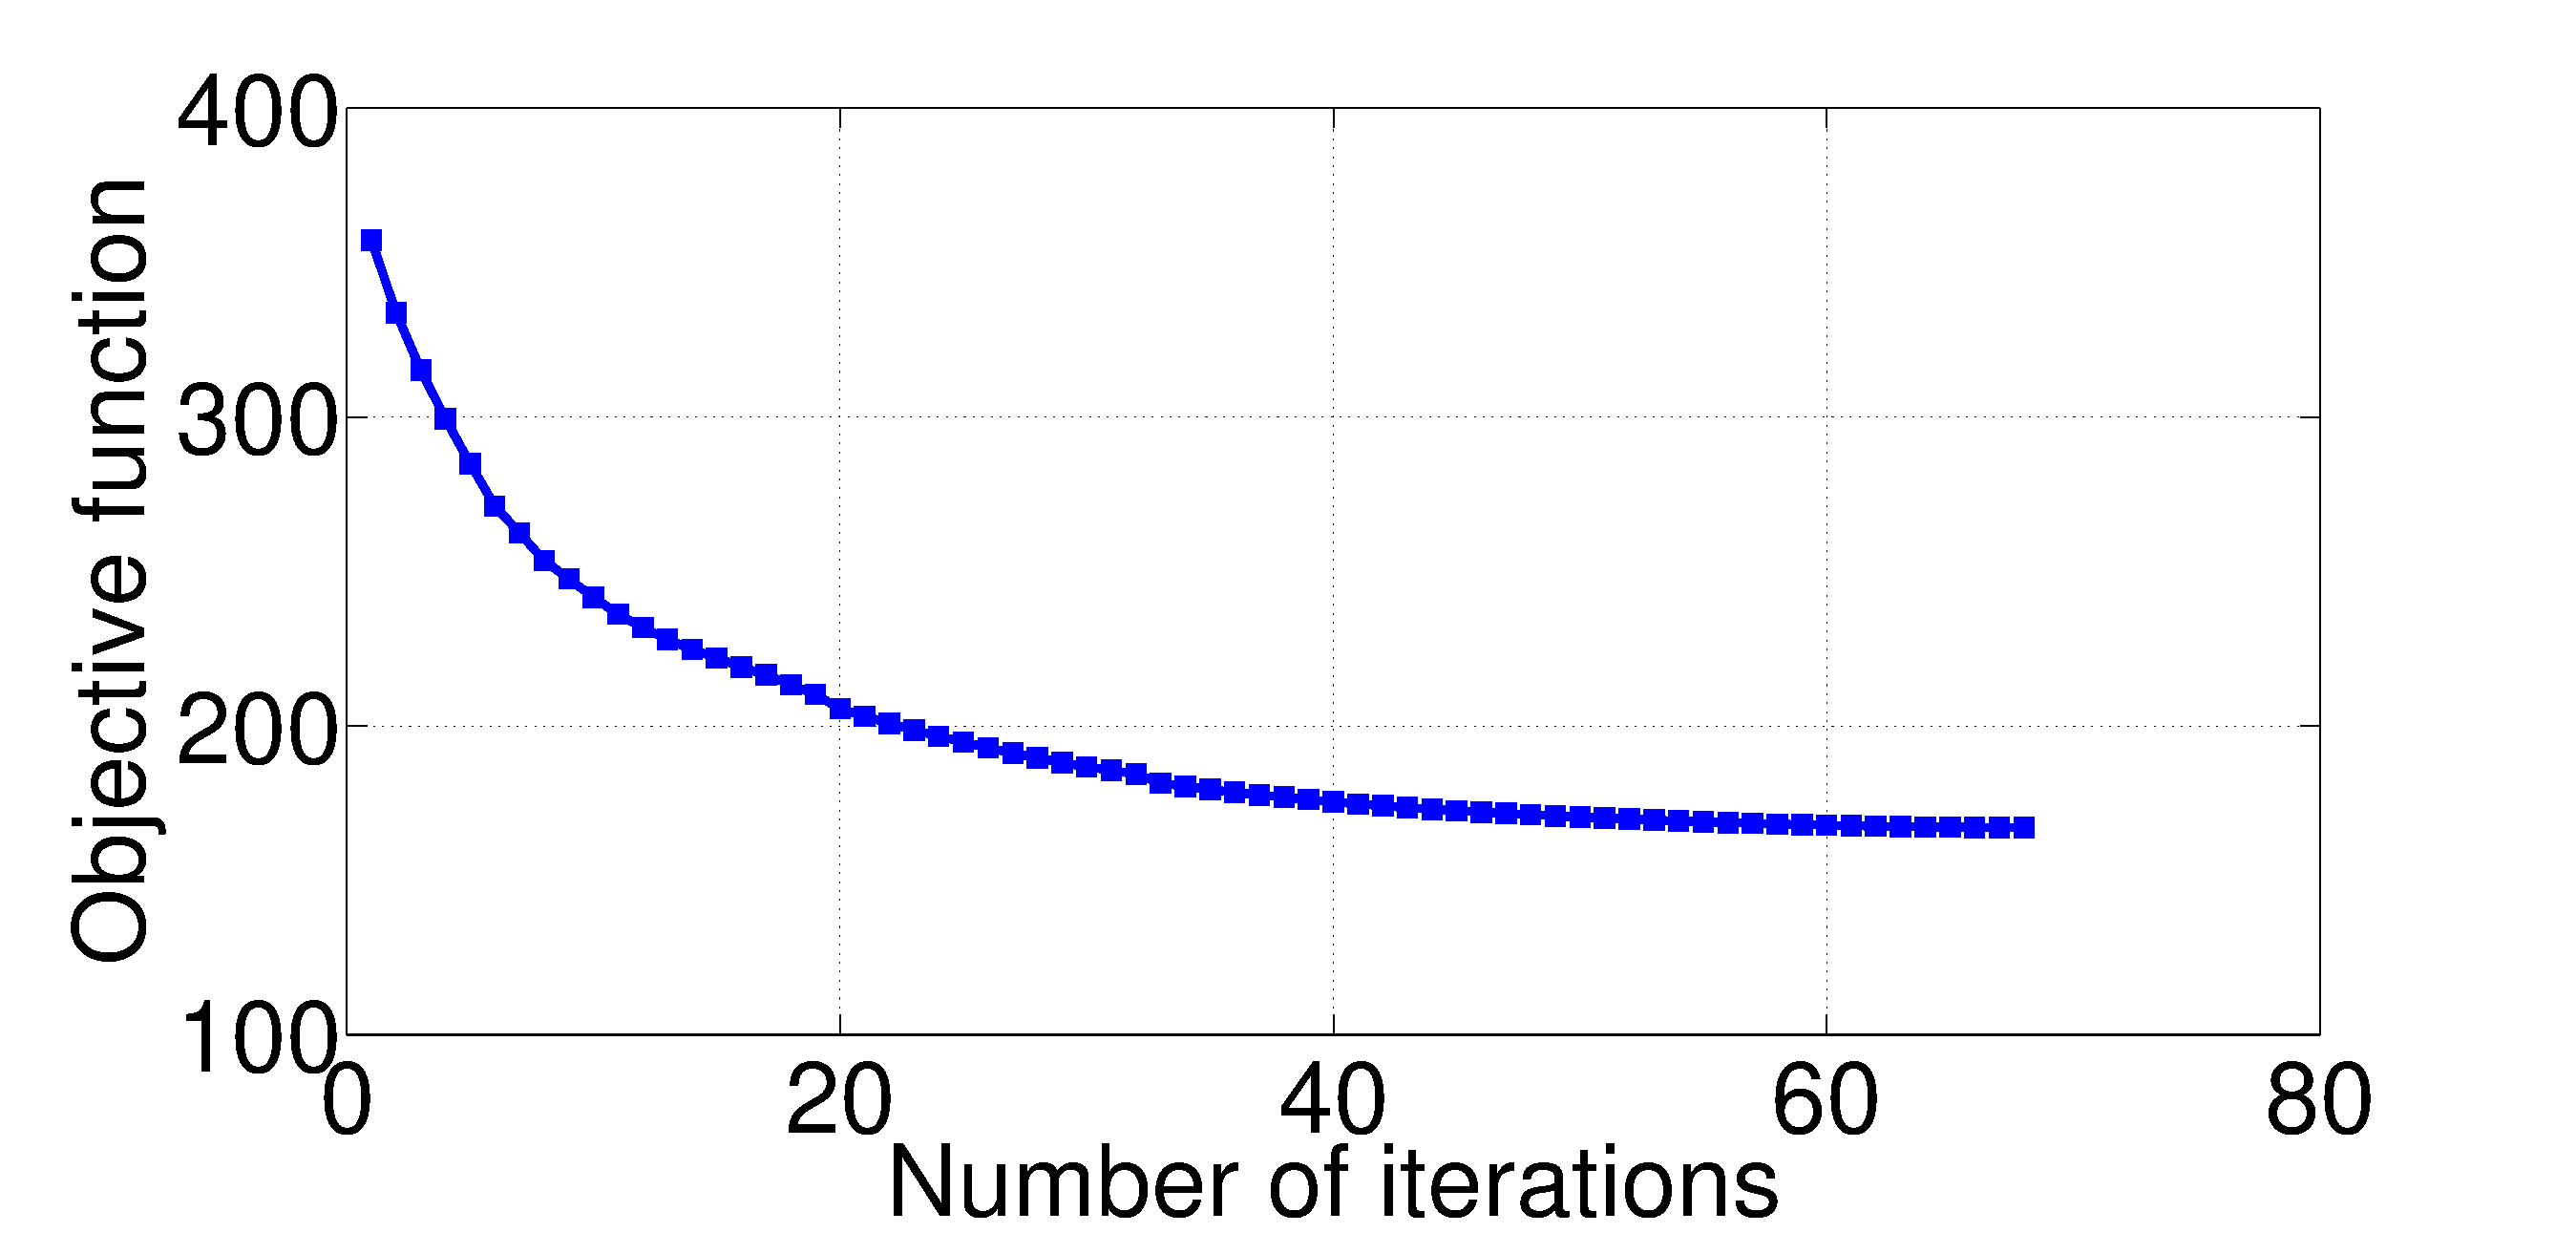
\includegraphics[width=\linewidth]{TagTree/LSWWW_objectivefnValuePerIteration}
\caption{The variation of the objective function~(\ref{eq:ObjFnWeightedHops}) with the number of iterations for a sample run on Flickr tag corpus.} 
\label{fig:ObjFun}
\endminipage\hfill
\minipage{0.32\textwidth}
  \includegraphics[width=\linewidth]{TPFlickr_rebuttal}
\caption{\hl{Average Tag Prediction Accuracies marginalized over $N_{Tags}$ for various methods for the tag prediction task on Flickr corpus. }} 
\label{fig:FWS117TagPredGraph}
\endminipage\hfill
\minipage{0.32\textwidth}%
  \includegraphics[width=\linewidth]{RebuttalGWS_TP}
\caption{\hl{Average Tag Prediction Accuracies marginalized over $N_{Tags}$ for various methods for the tag prediction task on Stock images corpus.}}
\label{fig:GWS30TagPredGraph}
\endminipage
\end{figure*}
}
\textbf{Flickr corpus:} We begin by choosing  the top $150$ most popular tags in a sample of Flickr images. After selecting only those tags that also occur in the WordNet database, we are left with 117 tags. These comprise the set $\mathcal{T}$. The total number of tags in an image, varies from 0 to 6 for most Flickr images. Since we need at least one tag to be seen and at least one to be predicted, we vary $N_{Tags}$  from 2 to 6. For each value of $N_{Tags}$, test images are selected which contain exactly $N_{Tags}$ tags. For each such image $i$, all combinations of $N_{Seen}$ tags are selected to comprise the observed tag set $\mathcal{T}_{i,Seen}$. Predictions are made as discussed in Section ~\ref{sec:TagPredUsingGraph} and performance of tag prediction task is measured using~(\ref{eq:TagPredAccuracy}). $N_{Seen}$ is varied from 1 through $(N_{Tags} - 1)$. Given values for $N_{Tags}$ and $N_{Seen}$, the Average Tag Prediction Accuracy is the Tag Prediction Accuracy using (\ref{eq:TagPredAccuracy}) averaged across test images. We define Overall Tag Prediction Accuracy as the mean of Average Tag Prediction Accuracy across all combinations of $N_{Tags}$ and $N_{Seen}$. 

The Overall Tag Prediction Accuracies for the various methods compared are shown in Table ~\ref{tab:TPFlickr117Summary}. Tables \ref{tab:TPFlickr117Random} through \ref{tab:TPFlickr117Jij} show the Average Tag Prediction Accuracies for various combinations of $N_{Tags}$ and $N_{Seen}$ for the individual methods discussed in Section \ref{sec:comparison} for Flickr corpus. For comparison, the Average Tag Prediction Accuracies marginalized over $N_{Tags}$ are shown in Fig.~\ref{fig:FWS117TagPredGraph}. Note that Google Distance refers to the method corresponding to Google Similarity Distance as outlined above. \hl{It can be seen that the LS-SA method outperforms all others and has its performance very close to that of the Symmetric sum based approach {\cite{sigurbjornsson2008flickr}}. It should be noted that the latter utilizes pair-wise similarities between tags as derived from the corpus and thus has space requirement of $O(N^2)$ which as discussed in Section {\ref{sub_sec:relatedWork}} is very high for large number of tags, i.e., for large $N$. Compared to this, the proposed approach has only $O(N)$ space requirement. } We will discuss in Section \ref{sec:Discussion} the reason why LS-SA leads to construction of a tree that outperforms the LS-WAH method. Google distance based method has performance close to that of LS-WAH while the tag tree based on WordNet hierarchy does not work very well for tag prediction task. As expected, random tag prediction performs the worst.
%One interesting observation from Table ~\ref{tab:TPFlickr117Summary} and Fig.~\ref{fig:FWS117TagPredGraph} is that even the unweighted version of ontological tag tree obtained using proposed data-driven approach performs far better than both random prediction and WordNet based graph (both weighted and unweighted). 
%Stating differently, the gain in performance is not merely a manifestation of having corpus-centric edge weights though they do improved the performance obtained for this task.

\comment{
\begin{table}[htbp]
\begin{center}
\caption{Overall Tag Prediction Scores for various methods for the tag prediction task on Flickr corpus. }
\label{tab:TPFlickr117Summary}
%\begin{tabular}{|p{4cm}|p{3.0cm}|}
\begin{tabular}{|c|c|}
		\hline
%		\textbf{Tag Prediction Algorithm} & \textbf{Avg Tag Prediction Score (in \%)}   \\ 
		\textbf{Tag Prediction} & \textbf{Prediction}\\ 
		\textbf{Algorithm} & \textbf{Score (\%)}\\ 
		\hline 
		 Random tag prediction   & 1.63  \\
		\hline
		 WordNet hierarchy & 4.92  \\
		\hline
%		3 & Minimum spanning tree formed using WordNet distances  & 4.7740  \\
%		\hline
%		3 & 2 + Local search using WordNet distances (Needed?) & 7.44  \\
%		\hline
%		5 & 3 + Local Search using WordNet distances (Needed?) & 4.2622  \\
%		\hline
		 (Weighted) WordNet hierarchy  & 5.41  \\
		\hline
%		7 & 3 + Edge Weights (WordNet Distances)  & 5.1941  \\
%		\hline
%		8 & 4 + Edge Weights (WordNet Distances) (Needed?) & Pending  \\
%		\hline
%		9 & 5 + Edge Weights (WordNet Distances)  (Needed?) & Pending  \\
%		\hline
%		5 & 2 + Edge weights (Inverse of Jaccard Similarity) & 6.9   \\  
%		\hline
%		10 & 3 + Edge weights (Inverse of Jaccard Similarity) & ---  \\
%		\hline
		 LS on WordNet hierarchy & 28.61  \\
		\hline
%		11 & 3 + Local Search using Jaccard Similarity & 18.1985  \\
%		\hline
		 (Weighted) LS on WordNet hierarchy   &  35.75  \\
		\hline
%		13 & 11 + Edge Weights (Inverse Jaccard Similarity)   & 32.9313  \\
%		\hline
%		11 & 8 + Edge Weights (WordNet Distances)   & ---  \\
%		\hline
%		12 & 9 + Edge Weights (WordNet Distances)   & ---  \\ 
%		\hline
\end{tabular}
\end{center}
\end{table}
}

\begin{table}[htbp]
\fontsize{8pt}{1em}\selectfont
%\scriptsize
\begin{center}
\caption{Overall Tag Prediction Accuracy (\%) for various methods for tag prediction task on Flickr and Stock images corpora. }
\label{tab:TPFlickr117Summary}
%\begin{tabular}{|p{4cm}|p{3.0cm}|}
\begin{tabular}{|c|c|c|}
		\hline
		\textbf{Tag Prediction} & \textbf{Flickr} & \textbf{Stock images} \\ 
		\textbf{Method} & \textbf{corpus} & \textbf{corpus}\\ 
		\hline 
		 Random tag prediction   & 2.29  & 13.21 \\
		\hline
		 WordNet  & 7.95  & 22.67 \\
		\hline
		Google Similarity Distance & 34.02 & 40.05\\
		\hline 
		 LS - WAH &  31.53  & 48.06\\
		\hline
		LS - SA &  44.52 & 50.86 \\
		\hline
		\hl{Symmetric sum based} &  \hl{47.13} & \hl{54.71} \\
		\hline
\end{tabular}
\end{center}
\end{table}
%\vspace{-5mm}
\begin{figure}[htbp]
%\epsfig{width=9cm,figure=FWS117TagPredResultsusingSTForCol.eps}
%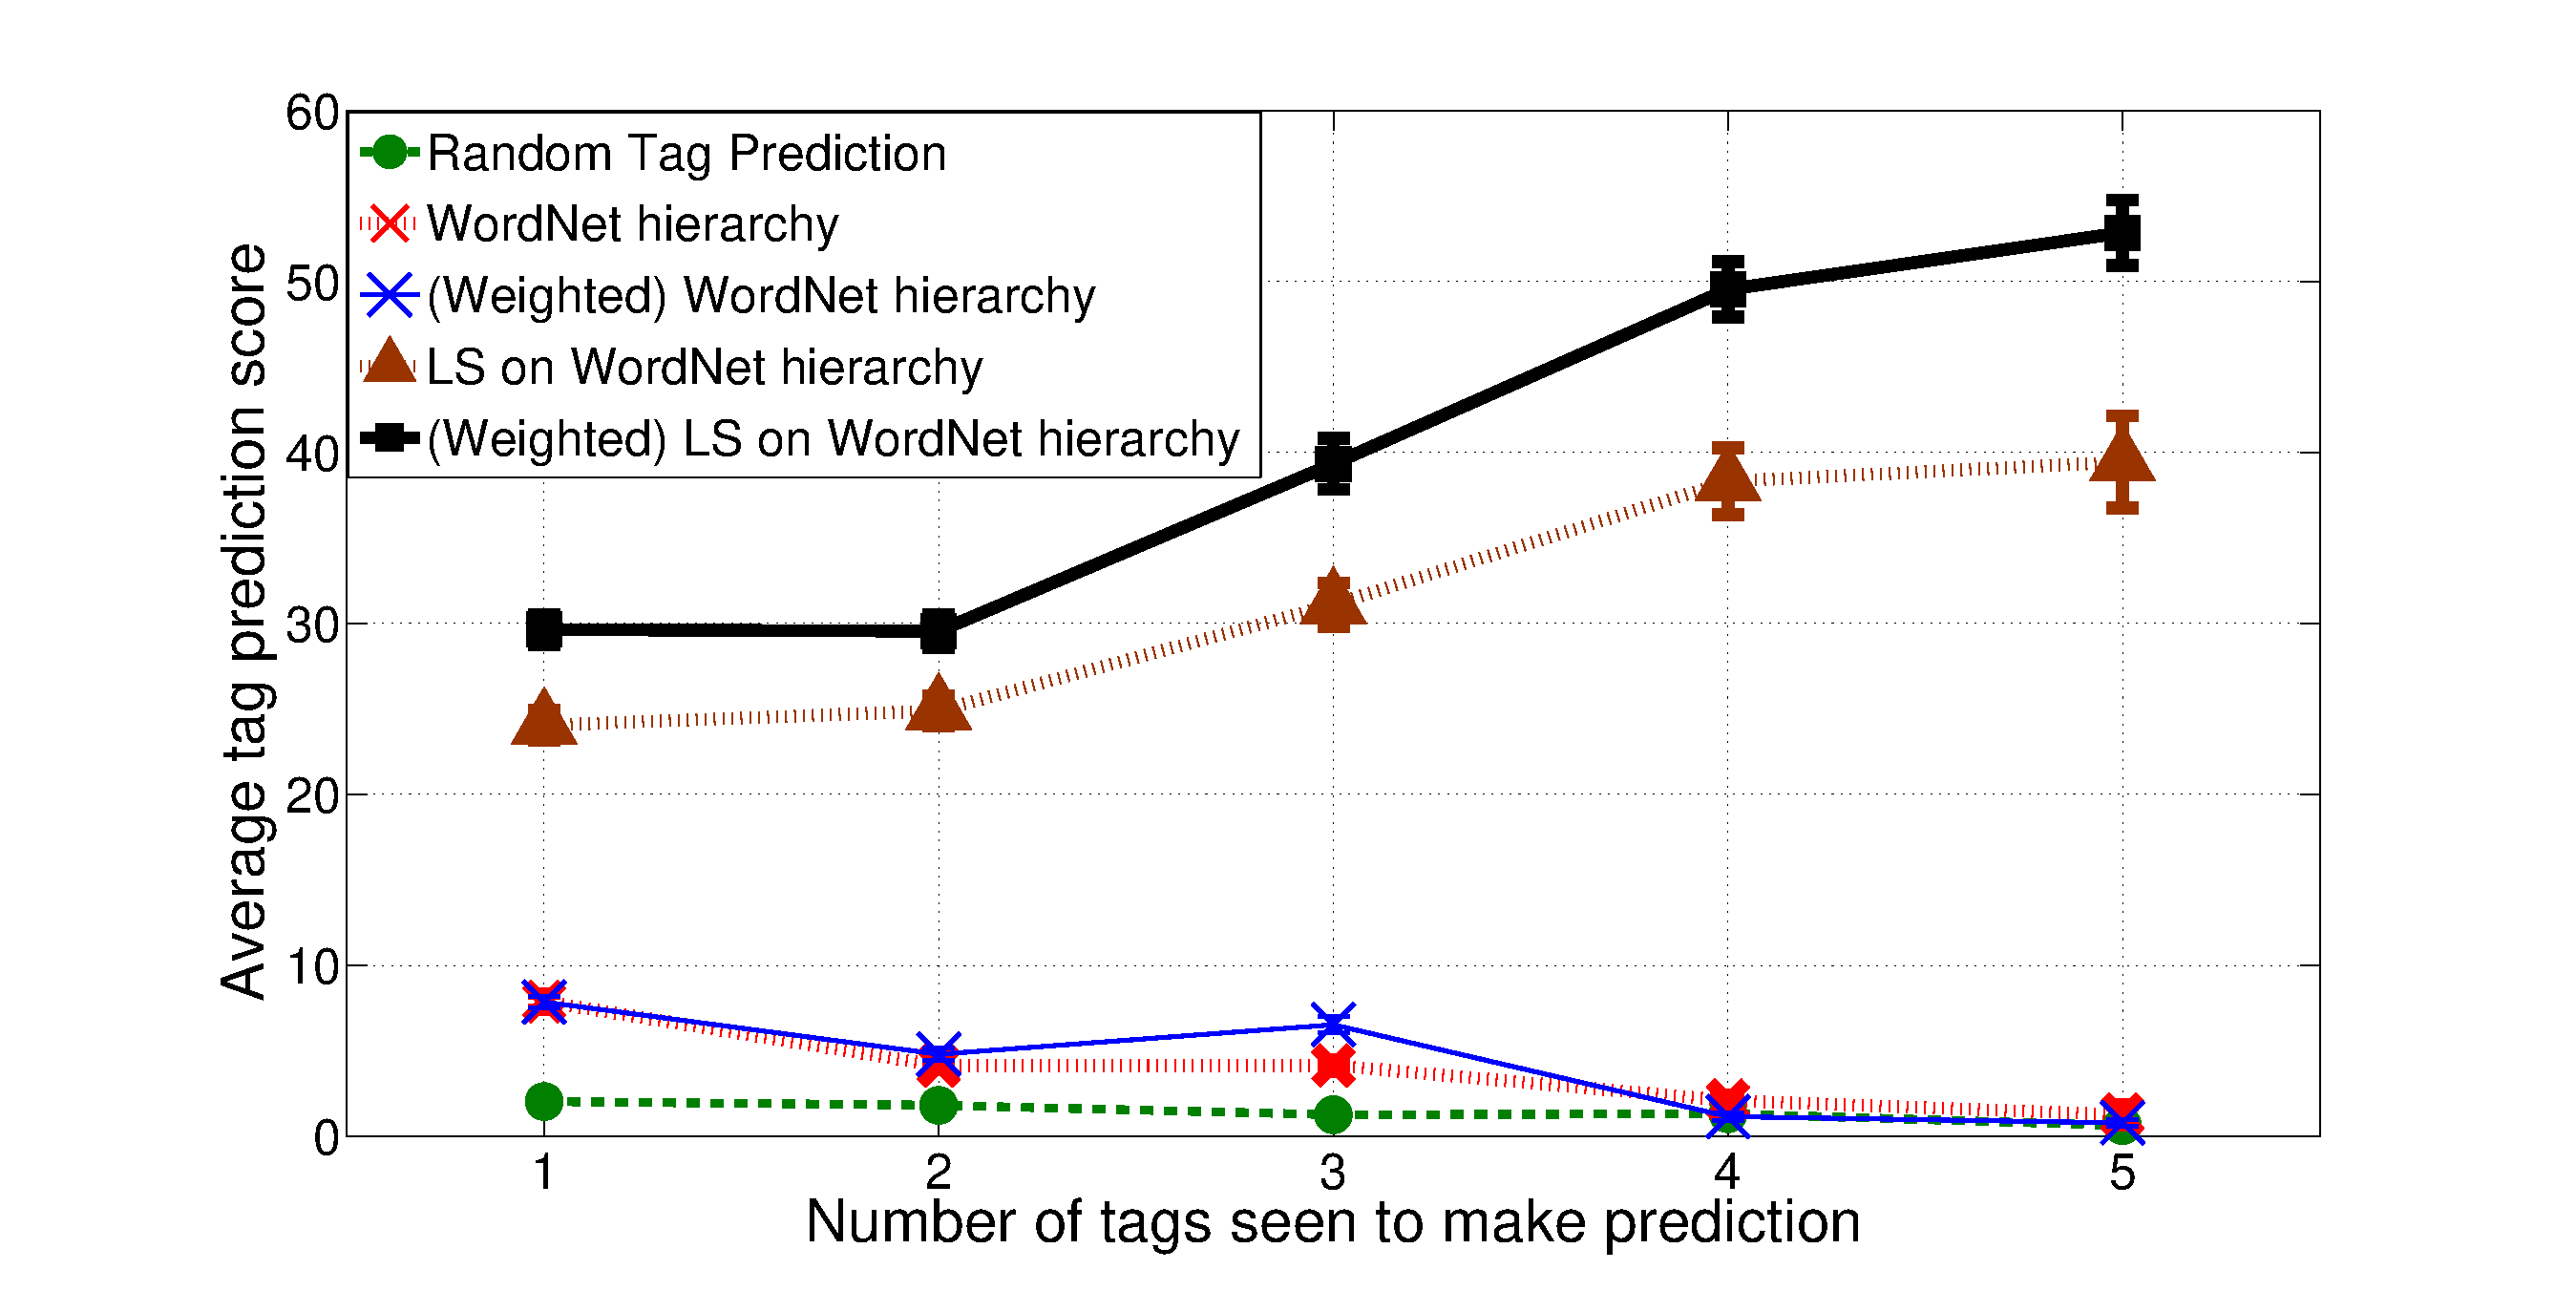
\includegraphics[width=\linewidth]{FWS117TagPredResultsusingSTForCol}
%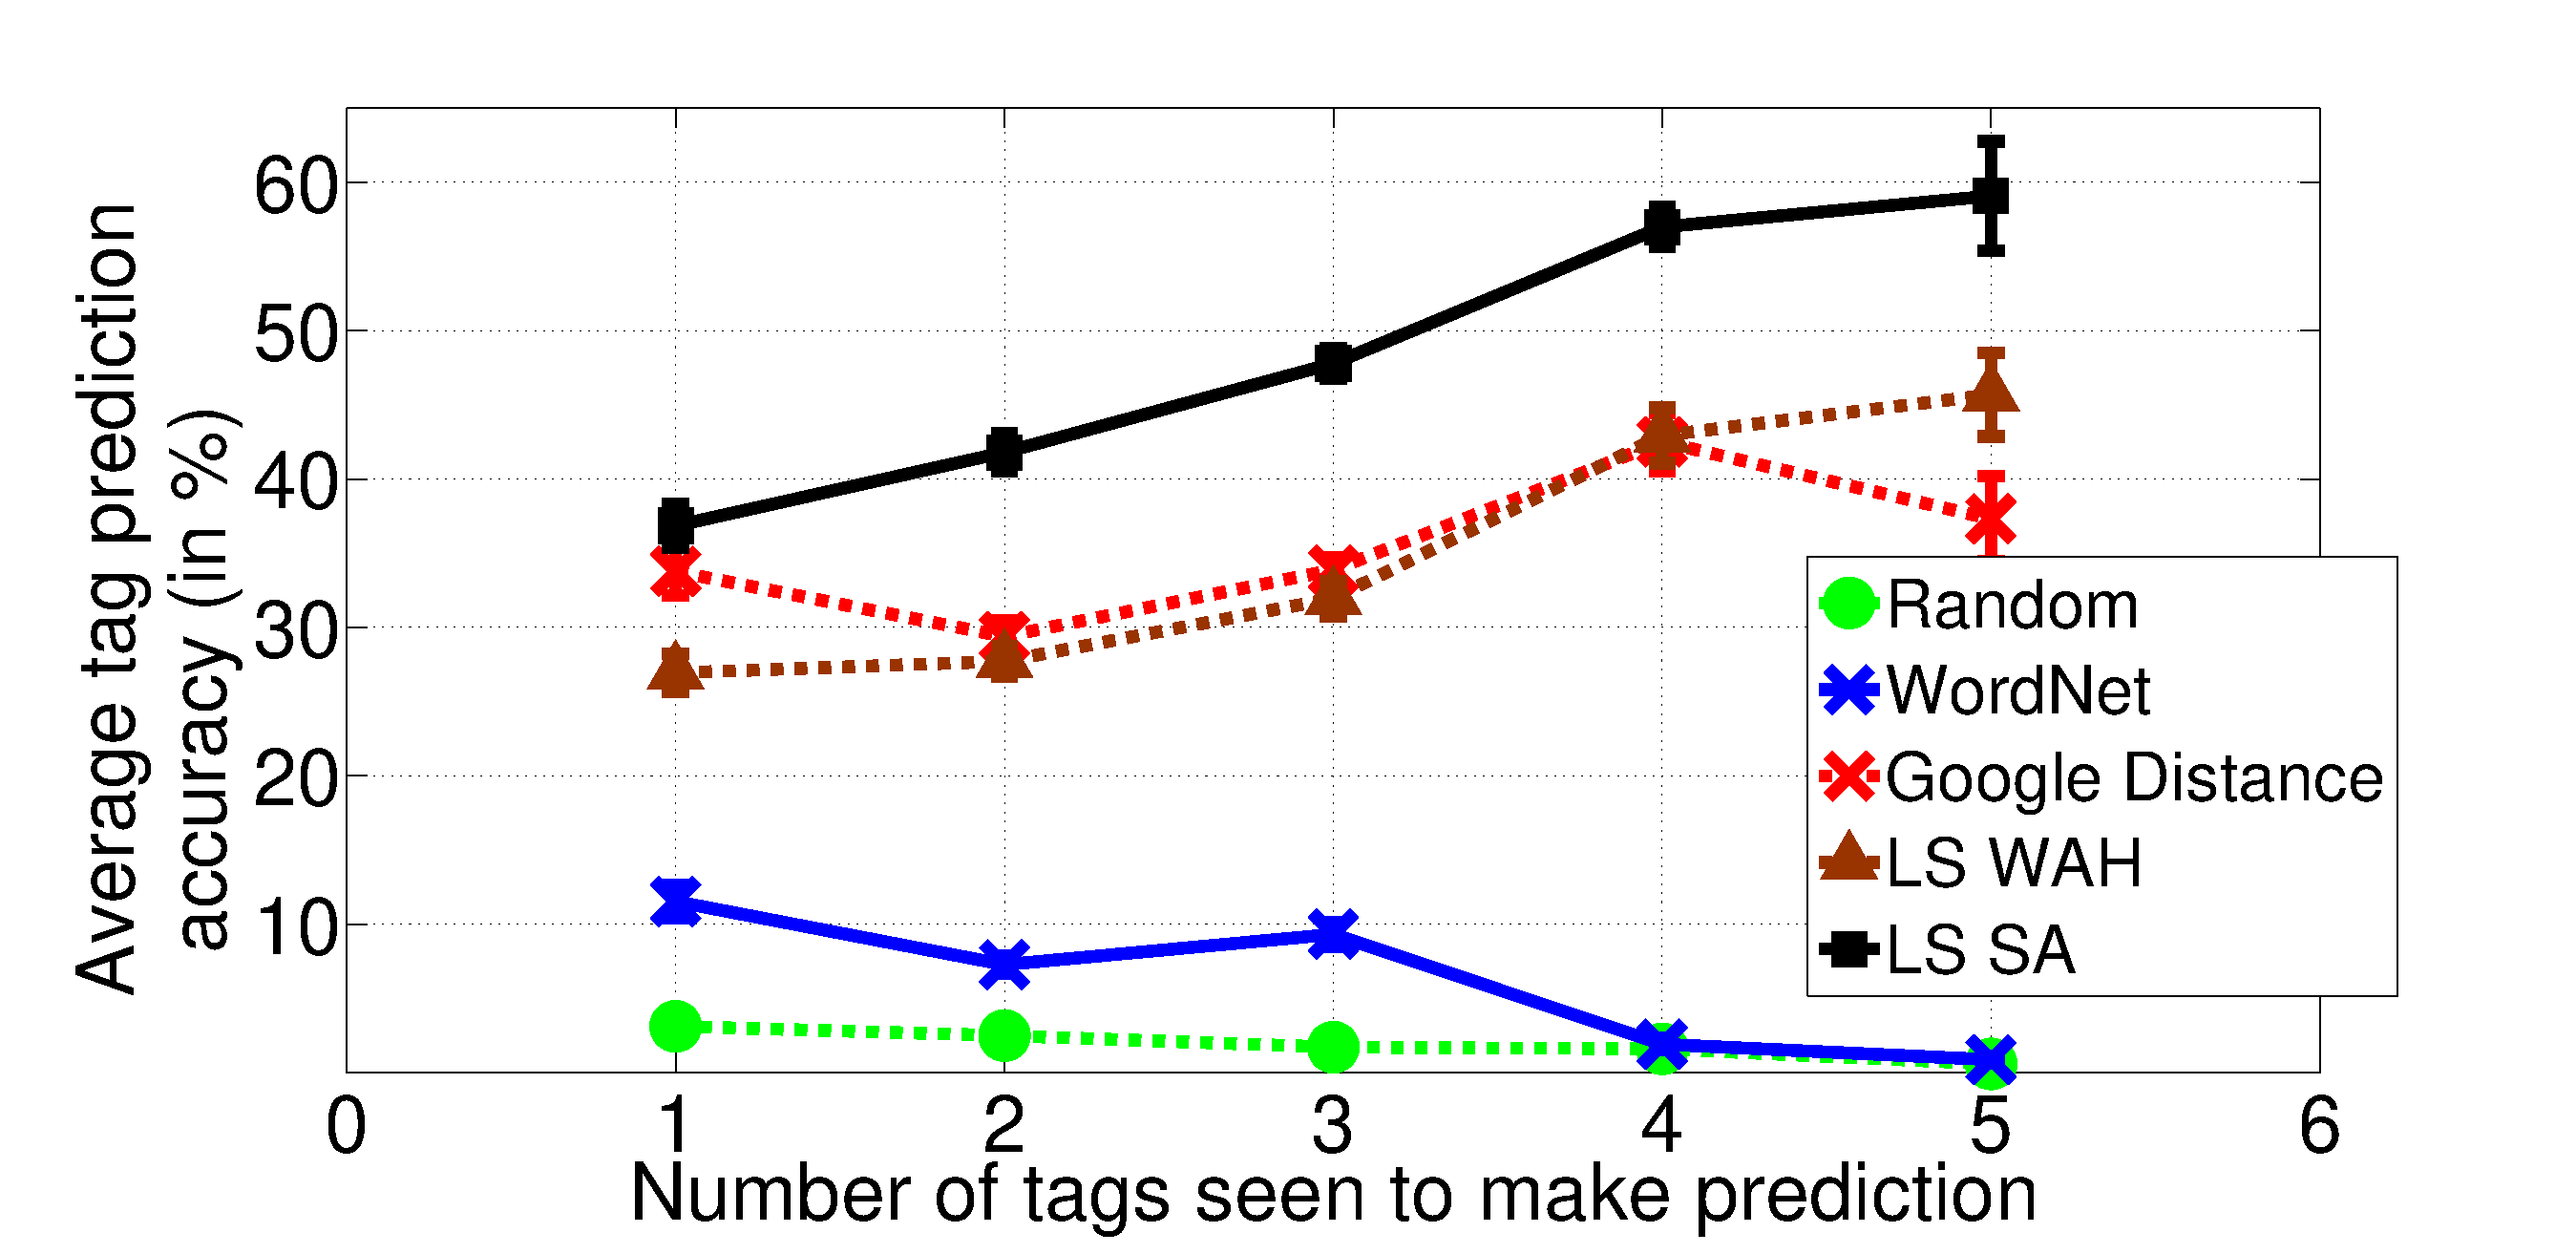
\includegraphics[width=\linewidth]{FlickrTPFig_journal}
\centering
\includegraphics[width=0.65\linewidth]{TagTree/TPFlickr_rebuttal}
\caption{\hl{Average Tag Prediction Accuracies marginalized over $N_{Tags}$ for various methods for the tag prediction task on Flickr corpus. Note that Google Distance refers to the method corresponding to Google Similarity Distance as outlined in }Section \ref{sec:comparison}.} 
\label{fig:FWS117TagPredGraph}
\end{figure}
\begin{table}
\fontsize{8pt}{1em}\selectfont
\begin{center}
\caption{Average Tag Prediction Accuracies (in \%) obtained using  Random method on Flickr corpus.}
%\vspace{-0.2in}
\label{tab:TPFlickr117Random}
\begin{tabular}{|p{2cm}|c|c|c|c|c|}
		\hline
		{$\boldsymbol{N_{Seen} \rightarrow}$} & &  &  &  &\\ 
		{$\boldsymbol{N_{Tags}} \downarrow $} & \textbf{1} & \textbf{2} & \textbf{3} & \textbf{4} & \textbf{5}   \\ 
		\hline 		
		\textbf{2} & 1.57 & - & - & - & -\\ 
		\hline
		\textbf{3} & 2.34 & 1.30 & - & - & -\\ 
		\hline
		\textbf{4} & 2.67 & 1.55 & 0.73 & - & -\\ 
		\hline
		\textbf{5} & 2.19 & 1.68 & 1.01 & 0.78 & -\\ 
		\hline
		\textbf{6} & 6.80 & 5.39 & 3.36 & 2.41 & 0.58 \\ 
		\hline
\end{tabular}
\vspace{-2mm}
\end{center}
\end{table}
\begin{table}
\fontsize{8pt}{1em}\selectfont
\begin{center}
\caption{Average Tag Prediction Accuracies (in \%) obtained using WordNet method on Flickr corpus.} 
\label{tab:TPFlickr117Wordnet}
\begin{tabular}{|p{2cm}|c|c|c|c|c|}
		\hline
		{$\boldsymbol{N_{Seen} \rightarrow}$} & &  &  &  &\\ 
		{$\boldsymbol{ N_{Tags}} \downarrow$} & \textbf{1} & \textbf{2} & \textbf{3} & \textbf{4} & \textbf{5}   \\ 	
		\hline
		\textbf{2} & 7.05 & - & - & - & -\\ 
		\hline
		\textbf{3} & 8.17 & 2.88 & - & - & -\\ 
		\hline
		\textbf{4} & 11.16 & 5.27 & 5.39 & - & -\\ 
		\hline
		\textbf{5} & 16.50 & 10.05 & 13.10 & 0.84 & -\\ 
		\hline
		\textbf{6} & 14.72 & 10.85 & 9.46 & 2.97 & 0.87 \\ 
		\hline
\end{tabular}
\vspace{-2mm}
\end{center}
\end{table}
\begin{table}
\fontsize{8pt}{1em}\selectfont
\begin{center}
\caption{Average Tag Prediction Accuracies (in \%) obtained using Google Similarity Distance method on Flickr corpus.} 
\label{tab:TPFlickr117Google}
\begin{tabular}{|p{2cm}|c|c|c|c|c|}
		\hline
		{$\boldsymbol{N_{Seen} \rightarrow}$} & &  &  &  &\\ 
		{$\boldsymbol{ N_{Tags}} \downarrow$} & \textbf{1} & \textbf{2} & \textbf{3} & \textbf{4} & \textbf{5}   \\ 	
		\hline
		\textbf{2} & 22.07 & - & - & - & -\\ 
		\hline
		\textbf{3} & 17.01 & 5.50 & - & - & -\\ 
		\hline
		\textbf{4} & 23.70 & 16.67 & 11.66 & - & -\\ 
		\hline
		\textbf{5} & 51.51 & 47.09 & 45.28 & 43.15 & -\\ 
		\hline
		\textbf{6} & 54.55 & 48.28 & 44.68 & 41.85 & 37.30 \\ 
		\hline
\end{tabular}
\vspace{-2mm}
\end{center}
\end{table}
\begin{table}[!htb]
\fontsize{8pt}{1em}\selectfont
\begin{center}
\caption{Average Tag Prediction Accuracies (in \%) obtained using LS-WAH method on Flickr corpus.} 
\label{tab:TPFlickr117LSWAH}
\begin{tabular}{|p{2cm}|c|c|c|c|c|}
		\hline
		{$\boldsymbol{N_{Seen} \rightarrow}$} & &  &  &  &\\ 
		{$\boldsymbol{ N_{Tags}} \downarrow$} & \textbf{1} & \textbf{2} & \textbf{3} & \textbf{4} & \textbf{5}   \\ 	
		\hline
		\textbf{2} & 16.13 & - & - & - & -\\ 
		\hline
		\textbf{3} & 11.53 & 5.51 & - & - & -\\ 
		\hline
		\textbf{4} & 14.91 & 10.96 & 7.17 & - & -\\ 
		\hline
		\textbf{5} & 42.76 & 42.94 & 39.69 & 36.95 & -\\ 
		\hline
		\textbf{6} & 49.37 & 51.48 & 49.00 & 48.89 & 45.69 \\ 
		\hline
\end{tabular}
\vspace{-2mm}
\end{center}
\end{table}
\begin{table}[!htb]
\fontsize{8pt}{1em}\selectfont
\begin{center}
\caption{Average Tag Prediction Accuracies (in \%) obtained using LS-SA method on Flickr corpus.}
\label{tab:TPFlickr117LSSA}
\begin{tabular}{|p{2cm}|c|c|c|c|c|}
		\hline
		%\textbf{$N_{Tags}$, $N_{Seen}$} & \textbf{1} & \textbf{2} & \textbf{3} & \textbf{4} & \textbf{5} \\ 
		{$\boldsymbol{N_{Seen} \rightarrow}$} & &  &  &  &\\ 
		{$\boldsymbol{N_{Tags}}\downarrow $} & \textbf{1} & \textbf{2} & \textbf{3} & \textbf{4} & \textbf{5}   \\ 
		\hline 		
		\textbf{2} & 25.87 & - & - & - & -\\ 
		\hline
		\textbf{3} & 20.34 & 21.65 & - & - & -\\ 
		\hline
		\textbf{4} & 26.09 & 28.96 & 26.43 & - & -\\ 
		\hline
		\textbf{5} & 52.33 & 54.79 & 54.82 & 53.16 & -\\ 
		\hline
		\textbf{6} & 59.57 & 61.78 & 62.10 & 60.81 & 59.07 \\ 
		\hline
\end{tabular}
\vspace{-2mm}
\end{center}
\end{table}
\begin{table}[!htb]
\fontsize{8pt}{1em}\selectfont
\begin{center}
\caption{\hl{Average Tag Prediction Accuracies (in \%) obtained using Symmetric sum method on Flickr corpus.}}
\label{tab:TPFlickr117Jij}
\begin{tabular}{|p{2cm}|c|c|c|c|c|}
		\hline
		%\textbf{$N_{Tags}$, $N_{Seen}$} & \textbf{1} & \textbf{2} & \textbf{3} & \textbf{4} & \textbf{5} \\ 
		{$\boldsymbol{N_{Seen} \rightarrow}$} & &  &  &  &\\ 
		{$\boldsymbol{N_{Tags}}\downarrow $} & \textbf{1} & \textbf{2} & \textbf{3} & \textbf{4} & \textbf{5}   \\ 
		\hline 		
		\textbf{2} &\hl{ 25.62} & - & - & - & -\\
		\hline
		\textbf{3} & \hl{21.19} & \hl{22.17} & - & - & - \\
		\hline
		\textbf{4} & \hl{28.69} & \hl{30.88} & \hl{28.12} & - & - \\
		\hline
		\textbf{5} & \hl{55.6} & \hl{57.88} & \hl{57.12} & \hl{54.27} & - \\
		\hline
		\textbf{6} & \hl{62.77} & \hl{65.48} & \hl{67.05} & \hl{66.35} & \hl{63.75} \\
		\hline
\end{tabular}
\vspace{-2mm}
\end{center}
\end{table}


%For completeness, we also provide the Average Tag Prediction Scores for various combinations of $N_{Tags}$ and $N_{Seen}$ in Tables~\ref{tab:TPFlickr117Random} - Table~\ref{tab:TPFlickr117GDWordNetSTJaccardWeight}. It is clear that the proposed approach greatly improves the performance compared to the WordNet based methods for all combinations of $N_{Tags}$ and $N_{Seen}$.
We provide examples of some test images from the Flickr corpus that had $N_{Tags}$=5 and $N_{Seen}$=2. Fig.~\ref{fig:positiveExs} shows a few test images for which LS-SA method made 100\% correct predictions. Fig. \ref{fig:negativeExs} shows test images that gave 0\% tag prediction accuracies. The corresponding sets of seen ($\mathcal{T}_{i,Seen}$), unseen ($\mathcal{T}_i \setminus  \mathcal{T}_{i,Seen}$), and the predicted tags ($\mathbb{P}_i$) are also provided. 


%Table~\ref{tab:TPFlickr117WordNetST}, the Average Tag Prediction Score for  $N_{Tags}=5$ and $N_{Seen}=3$ is only about 4.1\%. Compare this to the score obtained by proposed approach, as shown in Table~\ref{tab:TPFlickr117GDWordNetST}: 40.3\%! 





\textbf{Stock images corpus:} As in the Flickr corpus, we first select the set of most popular tags from the corpus of stock images that are also in WordNet. This produces a set $\mathcal{T}$, of 30 tags. Tables \ref{tab:TPGWS30Random} through \ref{tab:TPGWS30Jij} show the Average Tag Prediction Accuracies for various combinations of $N_{Tags}$ and $N_{Seen}$ for the tag prediction methods discussed in Section \ref{sec:comparison}. 
The Average Tag Prediction Accuracies marginalized over $N_{Tags}$ are shown in  Fig.~\ref{fig:GWS30TagPredGraph}, plotted as a function of $N_{Seen}$.  
%The total number of tags in an image, $N_{Tags}$ is varied from 2 to 10 such that $N_{Seen}$ varies from 1 to ($N_{Tags}-1$).  
Note that if $N_{Tags}$ is kept constant, increasing $N_{Seen}$ reduces the number of unseen tags (i.e., $\mathcal{T}_i \setminus  \mathcal{T}_{i,Seen}$), thus reducing the random chance of predicting a correct unseen tag from $\mathcal{T} \setminus \mathcal{T}_{i,Seen}$.  As a result of this phenomenon, a drop in performance for random prediction and other methods can be seen with increasing $N_{Seen}$. \\
\begin{figure}[!ht]
%\epsfig{width=10cm,figure=GWS20TagPredColumnMeanResultsForST.eps}
%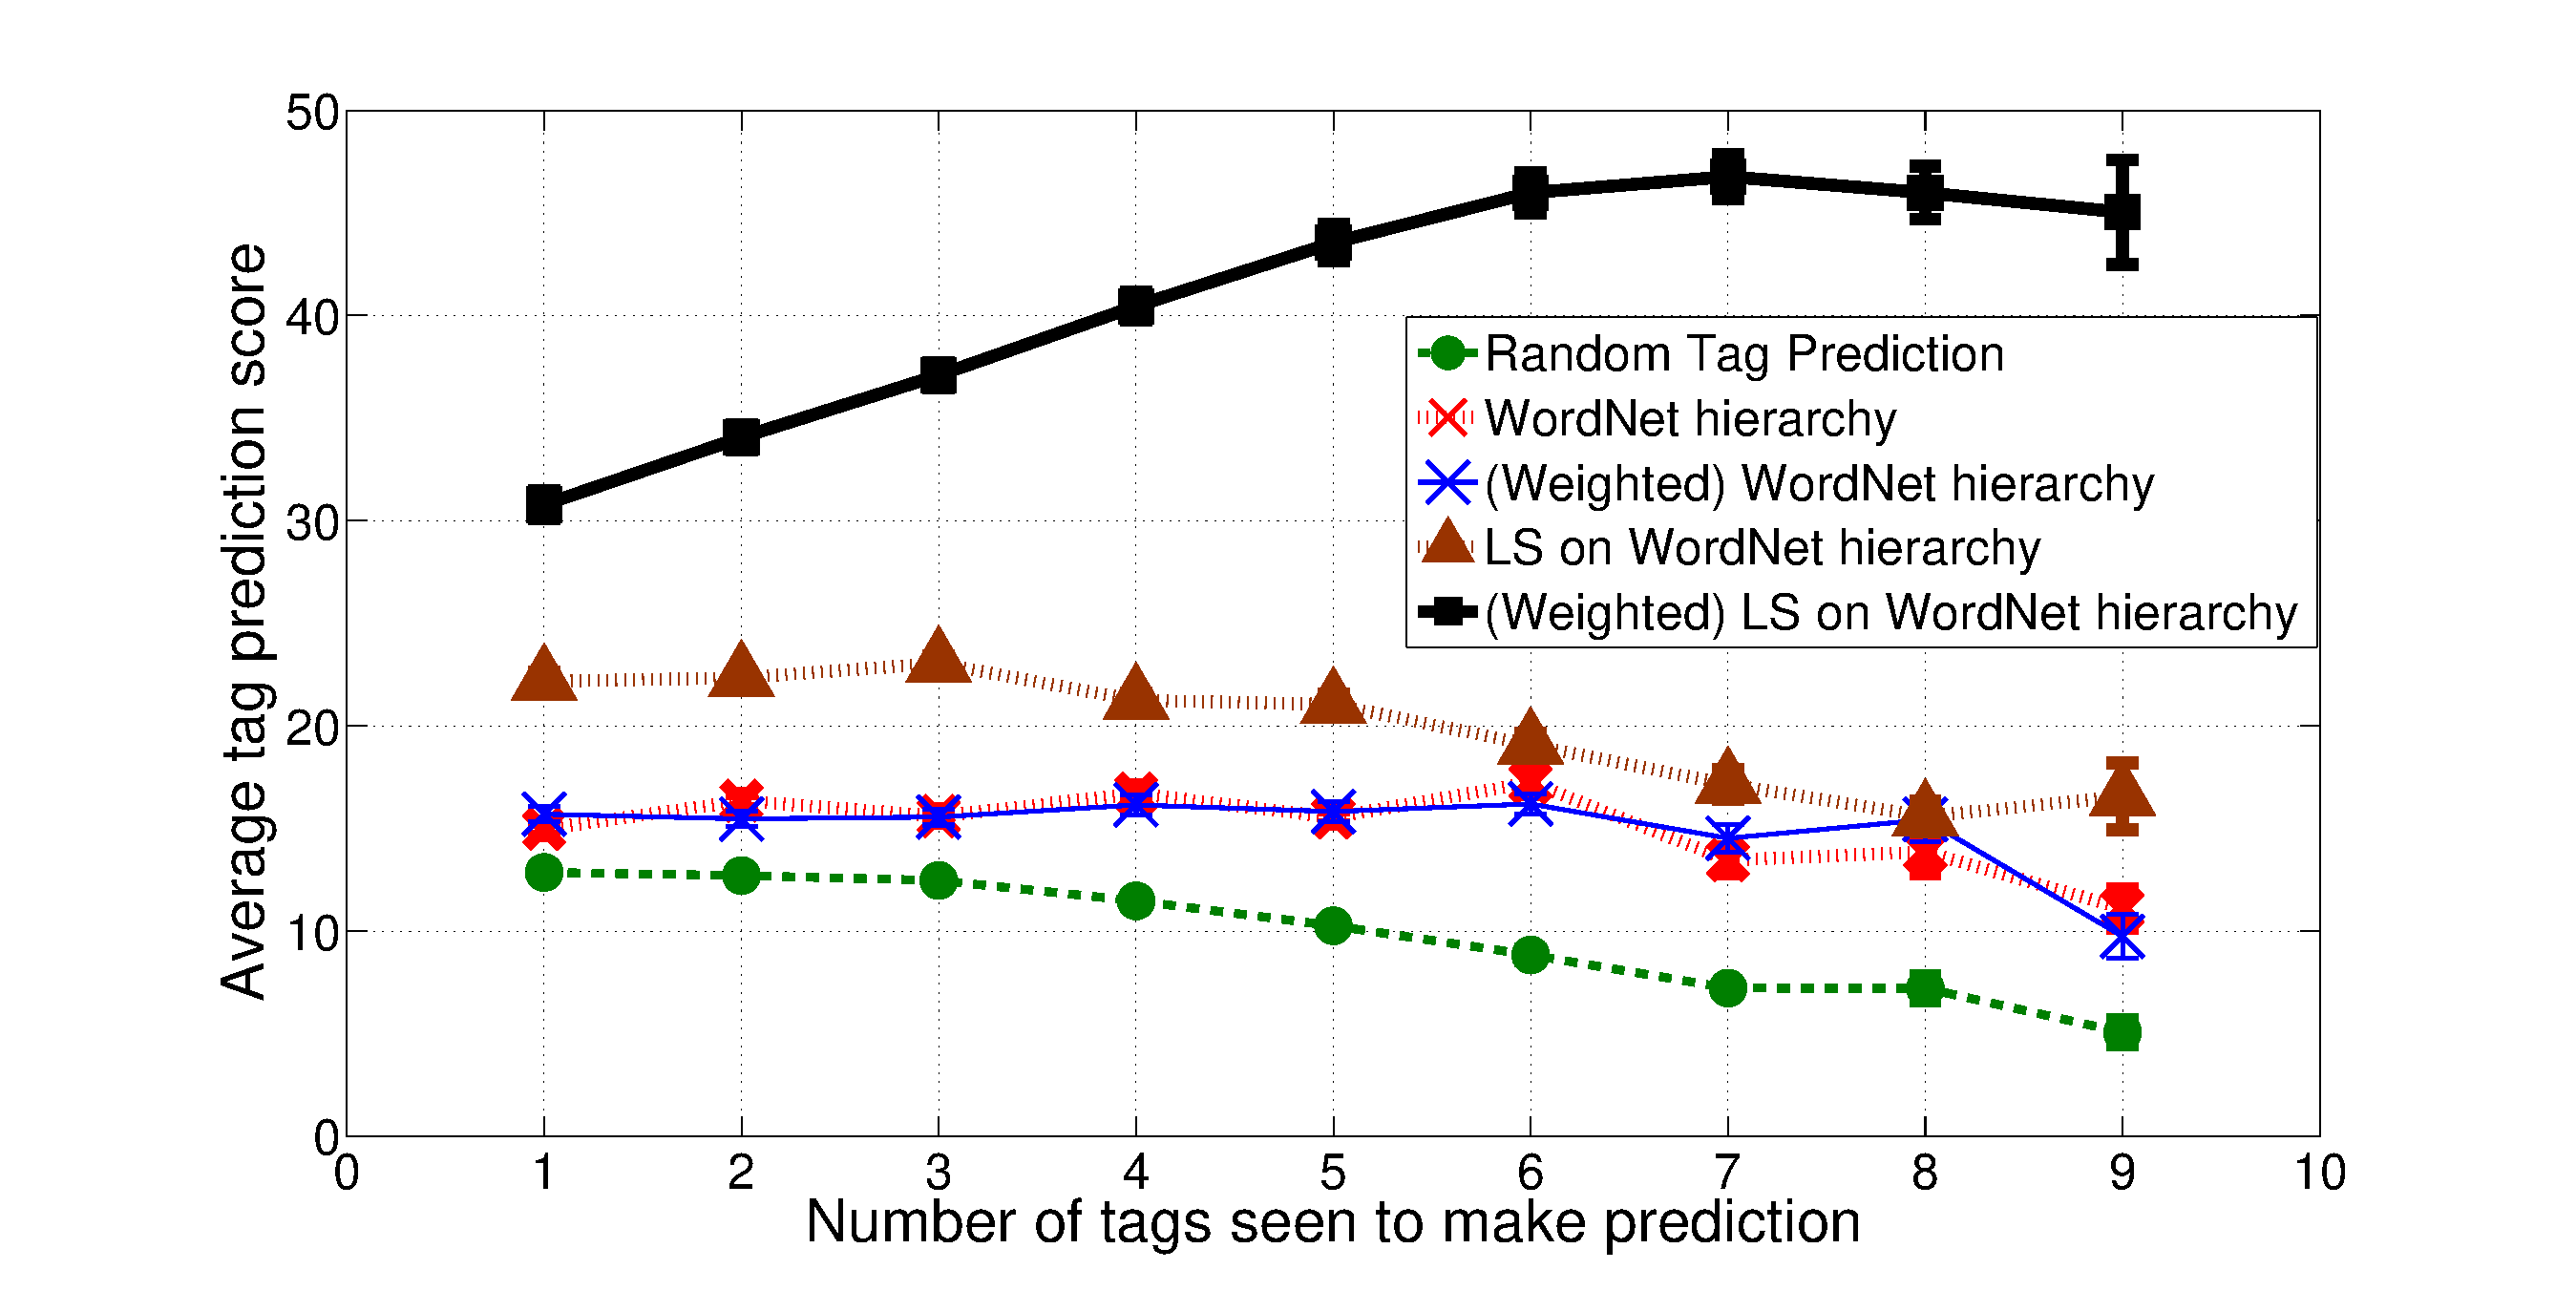
\includegraphics[width=\linewidth]{GWS20TagPredColumnMeanResultsForST}
%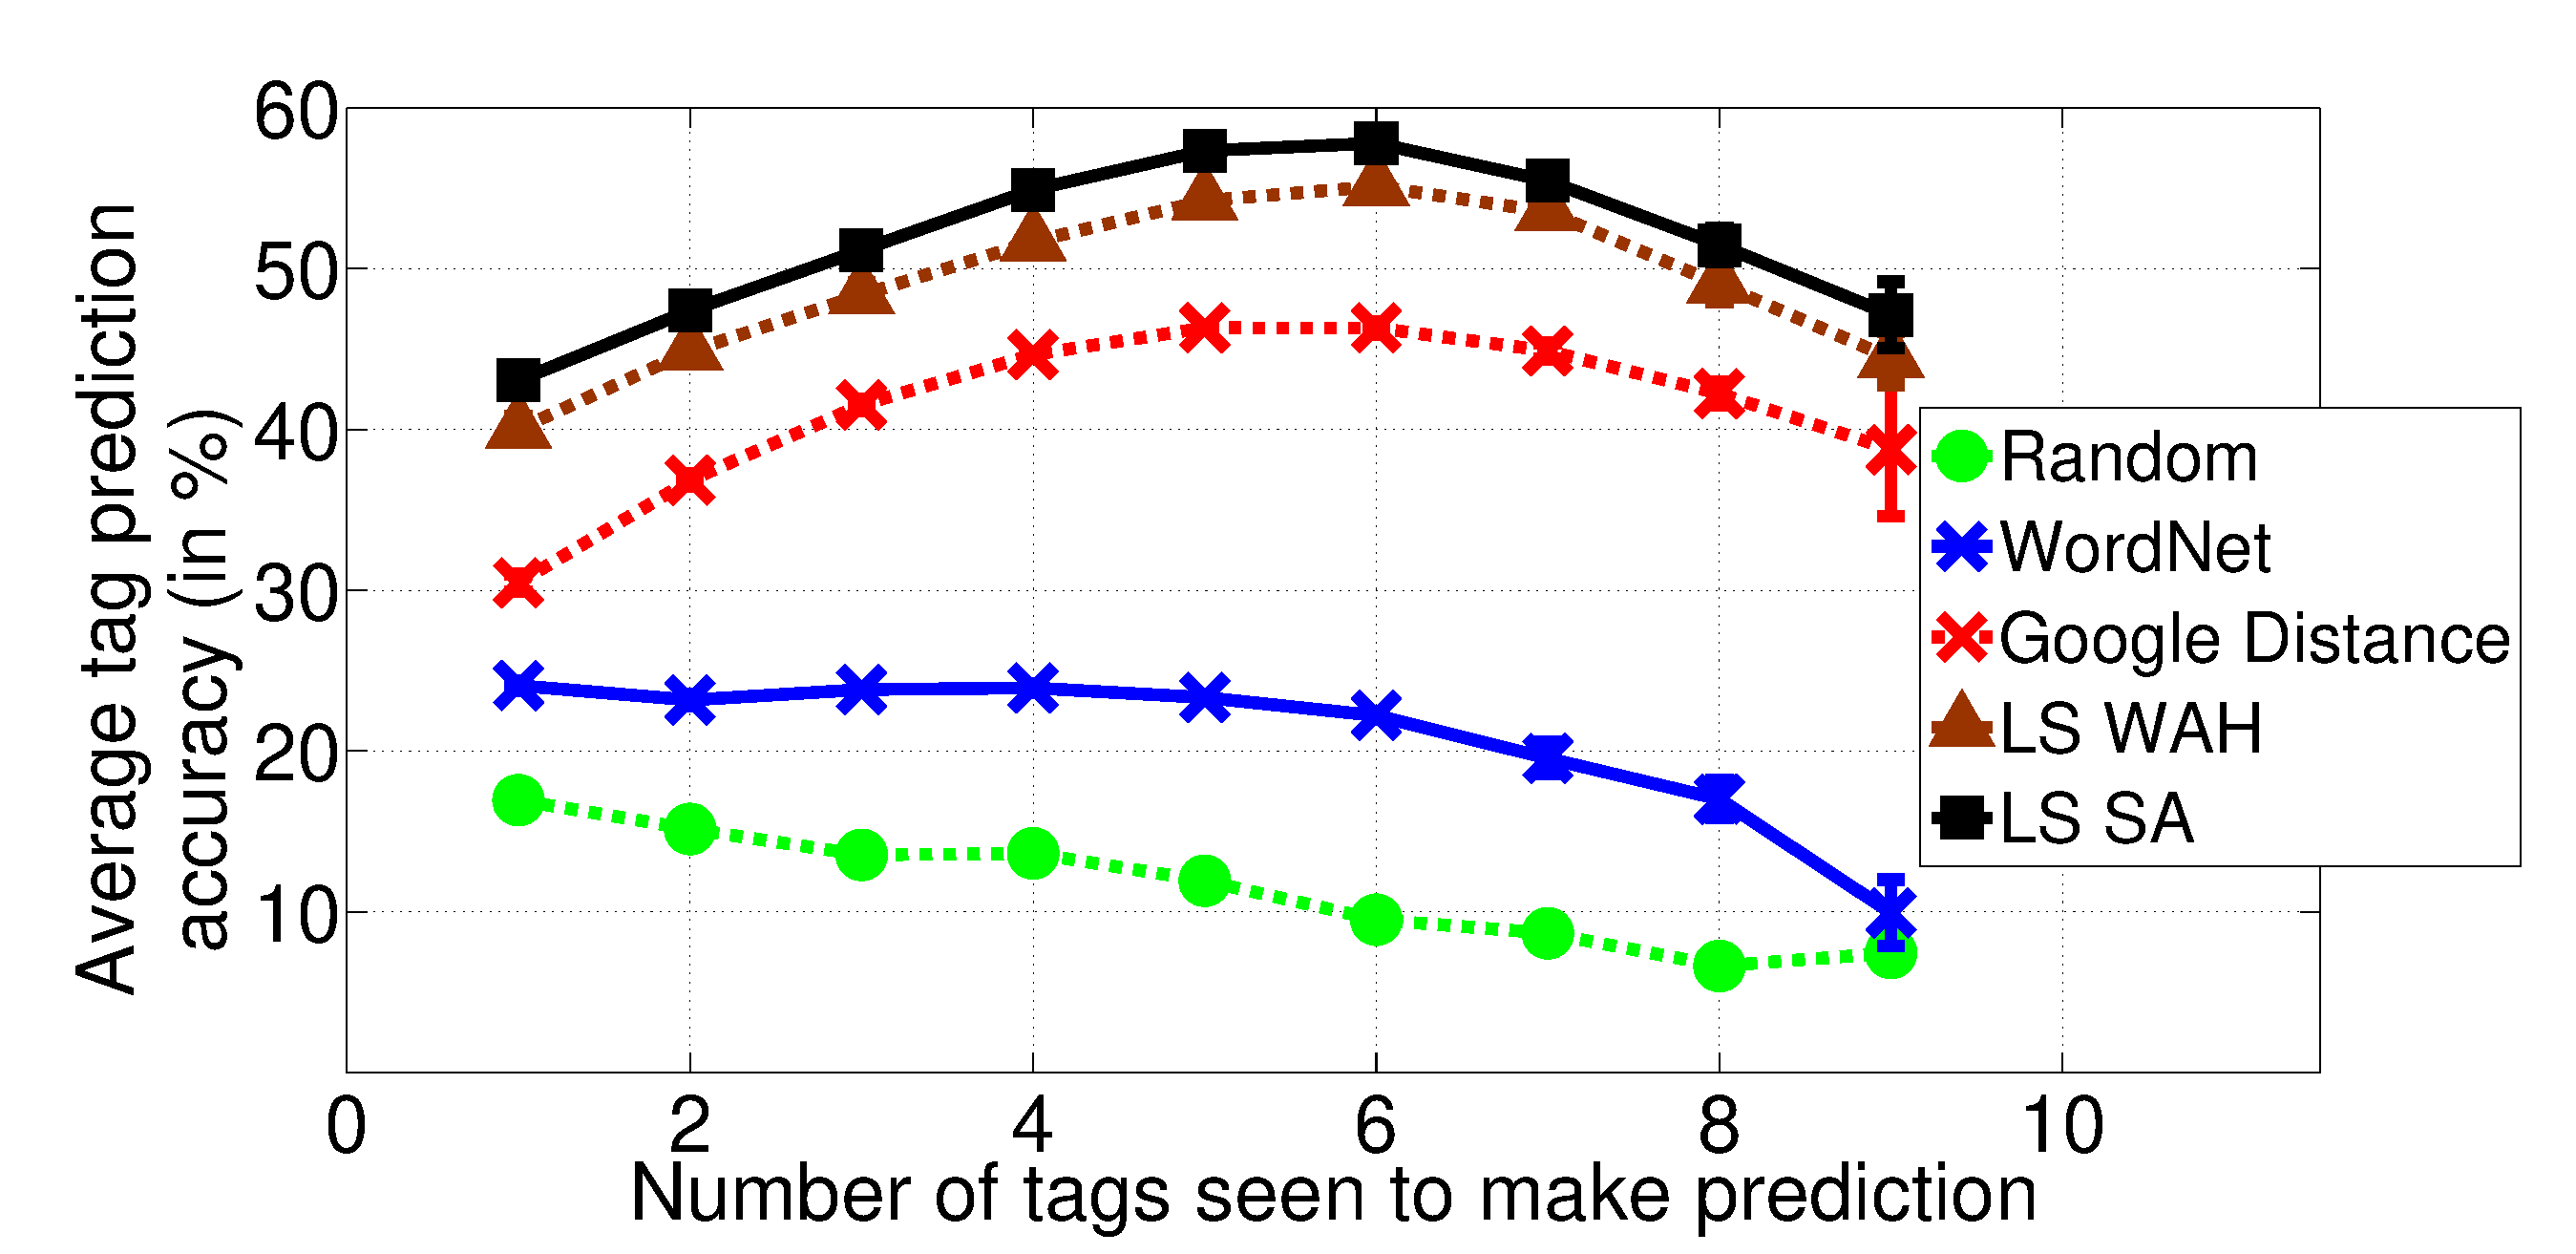
\includegraphics[width=\linewidth]{GWS30_tagPredFig_Journal}
\centering
\includegraphics[width=0.65\linewidth]{TagTree/RebuttalGWS_TP}
\caption{\hl{Average Tag Prediction Accuracies marginalized over $N_{Tags}$ for various methods for the tag prediction task on Stock images corpus.}}
\label{fig:GWS30TagPredGraph}
\end{figure}
\begin{table}[!htbp]
\fontsize{8pt}{1em}\selectfont
\begin{center}
\caption{Average Tag Prediction Accuracies (in \%) obtained using Random method on Stock images corpus.}
\label{tab:TPGWS30Random}
\begin{tabular}{|p{1.5cm}|p{0.5cm}|p{0.5cm}|p{0.5cm}|p{0.5cm}|p{0.5cm}|p{0.5cm}|p{0.5cm}|p{0.5cm}|p{0.5cm}|}
		\hline
		{$\boldsymbol{N_{Seen} \rightarrow}$} & &  &  &  & &  &  &  &\\ 
		{$\boldsymbol{N_{Tags}} \downarrow $} & \textbf{1} & \textbf{2} & \textbf{3} & \textbf{4} & \textbf{5}  & \textbf{6} & \textbf{7} & \textbf{8} & \textbf{9} \\ 
		\hline 		
		\textbf{2} & 1&-&-&-&-&-&-&-&- \\
		\hline
		\textbf{3} & 7&5.28&-&-&-&-&-&-&- \\
		\hline
		\textbf{4} & 11.3&5.8&4.9&-&-&-&-&-&-\\
		\hline
		\textbf{5} & 14.9&10.1&6.8&6.1&-&-&-&-&- \\
		\hline
		\textbf{6} & 19.1&12.9&10.1&9.5&3.1&-&-&-&- \\
		\hline
		\textbf{7} & 21.5&16.1&14.6&10.1&13.1&2.5&-&-&- \\ 
		\hline
		\textbf{8} & 20.7&17.8&11.8&12.7&6.4&9.6&2.3&-&- \\
		\hline
		\textbf{9} & 28.6&25.5&23&19.8&19.4&12.4&7&5.7&- \\ 
		\hline
		\textbf{10} & 28.3&27.6&23.5&23.5&17.7&13.6&16.7&7.6&7.4 \\ 
		\hline
\end{tabular}
\vspace{-2.5mm}
\end{center}
\end{table}
%It is clear that the tag trees built using the proposed approach outperform the baseline graphs constructed using WordNet for all values of $N_{Seen}$. 
%The detailed tables containing Average Tag Prediction Scores for all values of $N_{Tags}$ and $N_{Seen}$ are omitted for brevity but the trend is similar to the one observed for the Flickr corpus.
%\vspace{-5mm}
% The tag prediction score is higher when edge weights of constructed semantic graph are taken as Jaccard similarities between connecting tags. Readers should note however that the improvement is not entirely because of edge weights being Jaccard similarities. Rather, the edges in semantic graph obtain by proposed approach captures corpus specific information in a much more effective manner than semantics-based graphs such as obtained from WordNet. This can be verified by the consistent gap in performance for edge weights being 1, and Jaccard similarities. 
\begin{table}[!htbp]
\fontsize{8pt}{1em}\selectfont
\begin{center}
\caption{Average Tag Prediction Accuracies (in \%) obtained using WordNet method on Stock images corpus.}
\label{tab:TPGWS30Wordnet}
\begin{tabular}{|p{1.5cm}|p{0.5cm}|p{0.5cm}|p{0.5cm}|p{0.5cm}|p{0.5cm}|p{0.5cm}|p{0.5cm}|p{0.5cm}|p{0.5cm}|}
		\hline
		{$\boldsymbol{N_{Seen} \rightarrow}$} & &  &  &  & &  &  &  &\\ 
		{$\boldsymbol{N_{Tags}}\downarrow $} & \textbf{1} & \textbf{2} & \textbf{3} & \textbf{4} & \textbf{5}  & \textbf{6} & \textbf{7} & \textbf{8} & \textbf{9} \\ 
		\hline 		
		\textbf{2} & 1.9&-&-&-&-&-&-&-&- \\
		\hline
		\textbf{3} & 8.9&3.3&-&-&-&-&-&-&- \\
		\hline
		\textbf{4} & 14.2&10.9&3.4&-&-&-&-&-&- \\
		\hline
		\textbf{5} & 21.3&16.9&14.7&8.5&-&-&-&-&- \\
		\hline
		\textbf{6} & 28.4&22.8&22&16.7&9.8&-&-&-&- \\
		\hline
		\textbf{7} & 32.3&28.4&28.4&24.8&22.4&12.6&-&-&- \\
		\hline
		\textbf{8} & 35.7&33.3&32.7&30.7&27.6&23.8&13&-&- \\
		\hline
		\textbf{9} & 36.5&34.5&32.7&31.9&28.7&26.3&23.4&15.5&- \\
		\hline
		\textbf{10} & 37.4&35.2&32.9&30.8&28&26.1&22.3&18.5&9.9 \\
		\hline
\end{tabular}
\vspace{-2.5mm}
\end{center}
\end{table}
\begin{table}[~htp]
\fontsize{8pt}{1em}\selectfont
\begin{center}
\caption{Average Tag Prediction Accuracies (in \%) obtained using Google Similarity Distance method on Stock images corpus.}
\label{tab:TPGWS30Google}
\begin{tabular}{|p{1.5cm}|p{0.5cm}|p{0.5cm}|p{0.5cm}|p{0.5cm}|p{0.5cm}|p{0.5cm}|p{0.5cm}|p{0.5cm}|p{0.5cm}|}
		\hline
		{$\boldsymbol{N_{Seen} \rightarrow}$} & &  &  &  & &  &  &  &\\ 
		{$\boldsymbol{N_{Tags}}\downarrow $} & \textbf{1} & \textbf{2} & \textbf{3} & \textbf{4} & \textbf{5}  & \textbf{6} & \textbf{7} & \textbf{8} & \textbf{9} \\ 
		\hline 		
		\textbf{2} & 3.5&-&-&-&-&-&-&-&- \\
		\hline
		\textbf{3} & 11.2&8.4&-&-&-&-&-&-&- \\
		\hline
		\textbf{4} & 24&26.6&21.9&-&-&-&-&-&- \\
		\hline
		\textbf{5} & 32.3&39.8&39.7&35.2&-&-&-&-&- \\
		\hline
		\textbf{6} & 36.6&43.9&46.5&46.5&44.5&-&-&-&- \\
		\hline
		\textbf{7} & 39.4&44.8&47.8&49.5&49.5&48.5&-&-&- \\
		\hline
		\textbf{8} & 43.6&45.2&47.3&48.5&49.1&49&48.7&-&- \\
		\hline
		\textbf{9} & 41.9&43.5&44.4&45.4&45.9&45.8&45.2&44.9&- \\
		\hline
		\textbf{10} & 41.6&42.7&43.2&42.8&42.6&42&40.7&39.5&38.7 \\
		\hline
\end{tabular}
\vspace{-2.5mm}
\end{center}
\end{table}
\begin{table}[!htp]
\fontsize{8pt}{1em}\selectfont
\begin{center}
\caption{Average Tag Prediction Accuracies (in \%) obtained using LS-WAH method on Stock images corpus.}
\label{tab:TPGWS30LSWAH}
\begin{tabular}{|p{1.5cm}|p{0.5cm}|p{0.5cm}|p{0.5cm}|p{0.5cm}|p{0.5cm}|p{0.5cm}|p{0.5cm}|p{0.5cm}|p{0.5cm}|}
		\hline
		{$\boldsymbol{N_{Seen} \rightarrow}$} & &  &  &  & &  &  &  &\\ 
		{$\boldsymbol{N_{Tags}}\downarrow $} & \textbf{1} & \textbf{2} & \textbf{3} & \textbf{4} & \textbf{5}  & \textbf{6} & \textbf{7} & \textbf{8} & \textbf{9} \\ 
		\hline 		
		\textbf{2} & 7.8&-&-&-&-&-&-&-&- \\
		\hline
		\textbf{3} & 14.6&15.4&-&-&-&-&-&-&- \\
		\hline
		\textbf{4} & 20.5&22.6&22&-&-&-&-&-&- \\
		\hline
		\textbf{5} & 36.2&33.2&32.8&31.3&-&-&-&-&- \\
		\hline
		\textbf{6} & 49&47.6&45.2&43.3&41.5&-&-&-&- \\
		\hline
		\textbf{7} & 59.6&59.4&58.7&57.1&54.4&51.4&-&-&- \\
		\hline
		\textbf{8} & 62.3&63.5&63.2&62.8&61.4&58.2&54.9&-&- \\
		\hline
		\textbf{9} & 56.6&59.7&59.2&58.7&57.9&56.3&52.8&49.5&- \\
		\hline
		\textbf{10} & 53.5&57.6&57.4&56.8&56.1&54.7&52.9&48.5&44.4 \\
		\hline
\end{tabular}
\vspace{-2.5mm}
\end{center}
\end{table}
\begin{table}[!htp]
\fontsize{8pt}{1em}\selectfont
\begin{center}
\caption{Average Tag Prediction Accuracies (in \%) obtained using LS-SA method on Stock images corpus.}
\label{tab:TPGWS30LSSA}
\begin{tabular}{|p{1.5cm}|p{0.5cm}|p{0.5cm}|p{0.5cm}|p{0.5cm}|p{0.5cm}|p{0.5cm}|p{0.5cm}|p{0.5cm}|p{0.5cm}|}
		\hline
		{$\boldsymbol{N_{Seen} \rightarrow}$} & &  &  &  & &  &  &  &\\ 
		{$\boldsymbol{N_{Tags}}\downarrow $} & \textbf{1} & \textbf{2} & \textbf{3} & \textbf{4} & \textbf{5}  & \textbf{6} & \textbf{7} & \textbf{8} & \textbf{9} \\ 
		\hline 		
		\textbf{2} & 7.2&-&-&-&-&-&-&-&- \\
		\hline
		\textbf{3} & 13.38&11.1&-&-&-&-&-&-&- \\ 
		\hline
		\textbf{4} & 28.4&27&21.1&-&-&-&-&-&- \\
		\hline
		\textbf{5} & 44.5&41.9&38.5&35&-&-&-&-&- \\
		\hline
		\textbf{6} & 53.3&53.3&51.3&49.5&46.9&-&-&-&- \\
		\hline
		\textbf{7} & 61.7&63.2&62.6&60.8&58.3&56&-&-&- \\
		\hline
		\textbf{8} & 64.3&64.8&65.8&65.3&63.1&60.2&57.4&-&- \\
		\hline
		\textbf{9} & 59&60.2&60.8&61.1&60.8&58&55.3&52.3&- \\
		\hline
		\textbf{10} & 55.7&57.7&57.9&57.8&57.6&57&53.7&50.6&47.1 \\
		\hline
\end{tabular}
\vspace{-2.5mm}
\end{center}
\end{table}

\begin{table}[!htp]
\fontsize{8pt}{1em}\selectfont
\begin{center}
\caption{\hl{Average Tag Prediction Accuracies (in \%) obtained using the Symmetric sum approach on Stock images corpus.}}
\label{tab:TPGWS30Jij}
\begin{tabular}{|p{1.5cm}|p{0.5cm}|p{0.5cm}|p{0.5cm}|p{0.5cm}|p{0.5cm}|p{0.5cm}|p{0.5cm}|p{0.5cm}|p{0.5cm}|}
		\hline
		{$\boldsymbol{N_{Seen} \rightarrow}$} & &  &  &  & &  &  &  &\\ 
		{$\boldsymbol{N_{Tags}}\downarrow $} & \textbf{1} & \textbf{2} & \textbf{3} & \textbf{4} & \textbf{5}  & \textbf{6} & \textbf{7} & \textbf{8} & \textbf{9} \\ 
		\hline 		
		\textbf{2} & \hl{11.1} & -  & -  & -  & -  & -  & -  & -  & - \\
		\hline
		\textbf{3} & 16.9 & 17.7 & -  & -  & -  & -  & -  & -  & -\\ 
		\hline
		\textbf{4} & 32.1 & 32.5 & 29.7 & -  & -  & -  & -  & -  & - \\
		\hline
		\textbf{5} & 45.1 & 47.8 & 46.4 & 43.1 & -  & -  & -  & -  & - \\
		\hline
		\textbf{6} & 52.7 & 56 & 56.3 & 55.5 & 53.2 & -  & -  & -  & - \\
		\hline
		\textbf{7} & 62.1 & 64.6 & 64.9 & 63.9 & 62 & 59.9 & -  & -  & - \\
		\hline
		\textbf{8} & 64.5 & 68 & 68.1 & 67.8 & 65.8 & 63.1 & 60.5 & -  & - \\
		\hline
		\textbf{9} & 60.6 & 63.9 & 64.9 & 64.9 & 64 & 61.5 & 58.5 & 55.9 & - \\
		\hline
		\textbf{10} & 58 & 61.5 & 62.9 & 63.2 & 63.1 & 61.6 & 58.9 & 55 & \hl{52.3}\\
		\hline
\end{tabular}
\vspace{-2.5mm}
\end{center}
\end{table}


\indent The results indicates that the proposed local search paradigm based approach has successfully adapted the ontological tag tree obtained from WordNet to the Flickr or stock images corpus. \hl{We can obtain performance better than or close to that of other tag prediction approaches, while having several orders of savings in the space requirement. } We next describe the second data-driven task used for evaluation of tag trees. 
\subsection{Efficient Classification Task}
\label{sec:effClassification}
\hl{We consider the problem of efficiently associating tags with resources based on the resource content. For domains where it is feasible to extract features from the resource and to train concept detectors, we show how tag trees can be utilized to determine which concept detectors should be applied on a given test resource. We demonstrate this using annotated image corpora and utilize different modalities to represent the content of a given resource. }
Given a test image, $i$ from the corpus without any associated tags or keywords, we predict which of the $N$ tags are applicable to the image. By letting each of the $N$ tags correspond to a category or class, this is equivalent to a multi-class, multi-label classification task. Let us assume that one-vs-all binary classifiers are available for each tag class - these take the image instance $i$ as input and can predict $P(j \mid i)$ where class $j$ corresponds to tag $t_j$. We can use this to predict whether or not a tag $t_j$ should be associated with image $i$ based on whether $P(j \mid i)$ is greater than an appropriate threshold $\theta$ or not. 

The naive approach to predict all tags applicable to $i$ would be to test each of the $N$ classifiers on $i$ and accumulate those tags for which the predictions by the corresponding classifiers exceed $\theta$. \hl{Some works such as {\cite{li2013classifying}} propose techniques to make classification of images faster. However in order to do this, these works require re-training of classifiers and cannot utilize existing classifiers for each tag. 
%For example {\cite{li2013classifying}} proposes an approach to select positive and negative examples determined most relevant with respect to a given concept. 
Contrary to these, in the proposed approach, we can utilize pre-trained classifiers corresponding to different tags. Other works such as the image annotation application in {\cite{wu2008flickr}} associate a test image with tags based on applying all concept detectors on the test image and then combining the predictions. However such approaches require applying all $N$ classifiers to a given test image and are hence inefficient for a large number of tags. }
This process can be made more efficient by using the ontological tag tree on the set of tags. Once certain labels have been predicted for an image $i$, one can utilize the tree structure to decide which tags are more or less likely to be associated with the image. Thus the choice of the classifiers to test next on the image $i$, can be made in a more efficient manner.  Therefore, a tag tree that captures the relations between the tags more effectively, is expected to lead to more efficient performance by reaching the correct number of predicted tags with fewer number of binary classifications performed. The \emph{efficient classification task} is formulated to measure the classification efficiency in such a setting. 

\indent This evaluation task is formulated as follows. Given $N$ binary classifiers, the $j^{th}$ classifier predicts probability $P(j \mid i)$ of tag $t_j$ being associated with a test image $i$. $K$ binary classifications are performed for image $i$ and the set of tags that are predicted positive among those $K$ classifications, comprise the set of predicted tags $\mathbb{P}_{i,K}$ for image $i$ for given $K$. The ground truth set of tags that are associated with image $i$ as per the corpus, is denoted $\mathcal{T}_{i}$. We define performance of the classification task based on the Tag Recall as defined below.
%** Check if Recall can be defined like this? Or does it have to be wrt different instances? ** \\
\begin{equation} 
\text{Tag Recall} = \frac{\mid \mathcal{T}_i \cap \mathbb{P}_{i,K} \mid}{ \mid \mathcal{T}_i \mid} 
\label{eq:TagClassfnRecall}
\end{equation} 

Based on the above definition, the Tag Recall is monotonically increasing with $K$: as more than $K$ classifications are performed, the cardinality of the set of predicted labels can remain constant or increase, leading to a non-decreasing value for the Tag Recall. 

%\subsection{Baseline Methods}
%\label{subsec:baselines}
\indent The most naive way of choosing the order in which the $N$ classifications are performed, would be to choose each binary classifier randomly. A more sophisticated approach can be adopted by choosing the classifiers based on the decreasing order of their class priors in the training corpus, i.e., choosing the classifier corresponding to the most frequently occurring tag first, followed by the next popular tag, and so on. We refer to these methods as Random, and Prior-based respectively. Below we discuss how the classifiers can be chosen based on their priors and a given ontological tag tree. 

\subsubsection{Utilizing Ontological Tag Tree for Classification} 
\label{sec:EffClassifnUsingGraph}
Intuitively, the procedure for using an ontological tag tree to decide how to choose the classifiers, is similar to the approach for the tag prediction task. For image $i$, once certain tags are predicted as present, the tags in their proximity (as per the tag tree) have a higher chance of being present too, and the corresponding classifiers should be tested sooner. Similarly, the predicted absence of tags brings down the chance that tags in their proximity will be present. We define below a priority score for the tags that have not been tested for, based on their priors and the predictions for the tags that have been tested for. For image $i$ and tag tree $T$, we define 
\begin{equation} \label{eq:FastClassifyEqn} 
priority(j) = P_{prior}(j) + \sum_{c \in C_{tested}}  {(P( c \mid i)- \theta) \times  (1-dist'(c, j)) }
%\theta = 1. 
\end{equation}
where $dist'(c,j)$ is the distance $dist(c,j)$ as defined in Section \ref{sec:TagPredUsingGraph} for various methods, normalized with respect to its maximum value such that $dist'(c,j)$ varies between 0 and 1. $P_{prior}(j)$ is the prior probability of tag $t_j$, and $C_{tested}$ is the set of tags that image $i$ has been tested for. Algorithm~\ref{EffClassfnAlgo} utilizes (\ref{eq:FastClassifyEqn}) and presents the algorithm employed to decide the order of classifications for each image $i$. For a given image $i$ and given $K$, the set of labels predicted as present, i.e., $\mathbb{P}_{i,K}$ can be obtained using Algorithm~\ref{EffClassfnAlgo}. \\ 
\begin{algorithm}[!t]
\fontsize{8pt}{1em}\selectfont
\caption{Algorithm for Efficient Classification by using Ontological Tag Tree} 
\label{EffClassfnAlgo} 
\textbf{Input:} \\ 
$\cdot$ $C_j$: classifier for label $j \,$ corresponding to tag $t_j$ ($\forall j \in \mathcal{T} $), that can provide $P(j \mid i)$ for image $i$; threshold $\theta$ \\ 
$\cdot$ $P_{prior}(j)$: prior probability for tag $t_j$  \\
$\cdot$ $dist'(t,t')$: normalized inter-tag distances calculated based on given tag tree as outlined in Section~\ref{sec:EffClassifnUsingGraph}\\
$\cdot$ $K$: number of binary classifications to perform \\ 
\textbf{Initialize:} $L_{tested} $ = [ ]  \\
\textbf{Loop While} $\mid  L_{tested}  \mid$  $ \le \; K$  \\
\hspace*{5mm} $\cdot$ Calculate priority score for all tags in $(\mathcal{T} \setminus L_{tested}  )$ \\
\hspace*{5mm} using (\ref{eq:FastClassifyEqn}) \\
\hspace*{5mm} $\cdot$ Test classifier $C_{\hat{j}}$ corresponding to tag $t_{\hat{j}}$  with highest \\
\hspace*{5mm} calculated priority score to get $P( \hat{j} \mid i)$. \\
\hspace*{5mm} $\cdot$  $L_{tested} = L_{tested} \cup \hat{j}$. \\
\textbf{EndWhile}. \textbf{Output:} $\mathbb{P}_{i,K} = \{ j: P(j \mid i) > \theta , \, \, \,  j \in  L_{tested} \} $ 
\end{algorithm}
\textbf{Flickr corpus:} We use the same set of 117 Flickr tags as described in Section ~\ref{subsec:TagPred}. In order to train image classifiers 500,000 Flickr training images are used. Each tag $t_j$ is treated as a class. Positive training images are those that associated with the corresponding tag $t_j$ and negative training are those that are not. We use a ratio of $1:10$ for number of positive instances to number of negative instances for each class. SIFT features~\cite{lowe} are used to train binary SVM classifiers for each class. We provide results for the Random and Prior-based methods as discussed in Section~\ref{sec:effClassification}, and for methods 2 through 6 described in Section~\ref{sec:comparison} using the approach outlined in Section~\ref{sec:EffClassifnUsingGraph}. For $\theta = 0.5$, the Tag Recall observed with varying number of classifiers tested, i.e., $K$, are shown in Fig.~\ref{fig:EfficientTagPredGraphFlickr}. \hl{Note that {\cite{sigurbjornsson2008flickr}} does not utilize the symmetric similarities for an application as proposed in Section {\ref{sec:effClassification}}, however we utilize the symmetric jaccard similarities as per Algorithm ({\ref{EffClassfnAlgo}}) and compare against our approach for an understanding of the trade-off between performance and space requirement. 
%and compare the performance in order to provide an understanding of the .
 It is clear that for a given $K$, our approach outperforms the tag tree constructed from WordNet, the tag graph using Google Distance, and the ones that select classifiers randomly or solely based on prior. Performance of the LS-SA method is very close to that of the Symmetric sum method despite having several orders of savings in the space requirement as discussed in Sections {\ref{sub_sec:relatedWork}} and {\ref{subsec:TagPred}}}. For Tag Recall of around 4.4\%, the tag tree based on proposed approach (LS-SA) requires only 11 classifications compared to 21 for LS-WAH, 31 for Google Distance based, 51 for WordNet, 36 Prior based, and 61 when the classifiers are randomly selected. These correspond to 91\%, 182\%, 363\%, 227\%, 454\% \textit{additional} classifications used by these methods respectively, compared to the proposed method with Similarity Approximation (LS-SA). The WordNet based method performs worse than the Prior-based method, implying that the using semantics based distance with priors is less efficient than using priors alone. Visual-feature based image classification is a hard problem and the Tag Recall for 117 classes even after all 117 classifiers are tested, is observed to be less than 10\%. This is also a result of the individual classifiers and of the chosen threshold $\theta$. Note that the Tag Recall~(\ref{eq:TagClassfnRecall}) is different from recall of a class. For $\theta=0.5$, when all the classifiers are tested, the average recall over all classes is 10.5\% and the average precision is 15.9\%. \\
\indent A more lenient (i.e., lower) $\theta$ would lead to higher Tag Recall as can be seen in Fig.~\ref{fig:EfficientTagPredGraphFlickrLower}. $\theta=0.3$ corresponds to an average recall of 37.7\% and average precision of 4.9\%. A lower $\theta$ also implies less relative weight given to $P_{Prior}(j)$ in (\ref{eq:FastClassifyEqn}) and as a result, the WordNet method performs worse than even the Random method.  \\ 
\indent \textbf{Stock images corpus:} We perform experiments on the same corpus that was described in Section ~\ref{subsec:TagPred}. \hl{In order to show the applicability of our approach to different modalities that can be used to represent a given resource, we utilize
the textual caption accompanying the image $i$ to represent the image.} A TF-IDF based bag-of-words representation is used for each image, followed by binary SVM classifiers for each class. As in the case of Flickr, we present variation of Tag Recall with $K$ for various methods for $\theta=0.5$ in Fig.~\ref{fig:EfficientTagPredGraphGetty}. $\theta=0.5$ corresponds to an average recall of 73.6\% and average precision of 75.6\%. 
Our approach is seen to be able to better decide which classifiers to test, for a given $K$ and as a result, leads to higher Tag Recall for a fixed $K$. For Tag Recall of around 48\%, the tag tree based on the proposed approach (LS-SA) requires only 7 classifications compared to 9 for LS-WAH, 9 for Google Distance based, 15 for WordNet, 11 for only prior based and 21 when the classifiers are randomly selected. These correspond to 29\%, 29\%, 114\%, 57\%, 200\% \textit{additional} classifications used by these methods respectively, compared to the proposed method with Similarity Approximation (LS-SA).  \\ 
\indent It should be noted that the goodness of predictions i.e., the precision and recall obtained when all classifiers are tested, is essentially a property of the set of classifiers, which are the same for various methods used for this task. Based on the experiments, we have demonstrated that using ontological tag trees constructed through the proposed approach makes selection of classifiers much more efficient as compared to using purely semantics based tag tree or tag graphs built using commonly used techniques. \hl{We have also shown that we can achieve a performance almost as high as other approaches despite having several orders less space requirement. 
}
%conventionally, Tag Recall is reported with precision,  we only provide Tag Recall results since the objective of this task is to predict labels (tags) for given test image $i$ in as less binary classifications as possible. Also, the trade-off between precision and recall is essentially a property of the classifiers which are the same for various methods used for this task. \\
% \subsection{Evaluation of Semantic Graph Through Classification}  
% \label{EvalSemGraphClassifn}
% The caption associated with an image is used to represent it in a text-based bag-of-words representation. We prune words that occur in captions of less than two images, and remove stop words to construct a textual vocabulary of 21543 words. Each image is represented using TF-IDF numbers on the constructed vocabulary. 30 keywords are selected from Getty based on the keywords that were most popular, were not stop words, and occurred in WordNet hierarchy too. Each of the 30 keywords is considered a class for the purpose of evaluation. One-vs-rest Support Vector Machine is used to train a binary classifier for each class that can give probabilistic scores for its predictions. For training, we pick around 1000 images per class that are associated with the corresponding keyword. These comprise the positive instances. It is possible that the picked images are also associated with other keywords but we discard the overlap between classes (keywords) while training in order to avoid introducing any bias in the training set. The negative instances for a class comprises of the positive instances for other classes. For the testing set we collect around 1000 images per class and note all keywords associated with each testing image.  \\ 
% \indent \textit{Utilizing Semantic Graph for Classification} - Given is a semantic graph where each node $i$ corresponds to a class $i$. While training binary classifier for class $i$, we weigh the negative instances depending on their position in the semantic graph, with respect to the node $i$. Specifically, the instances of class $j$ are given a weight of $w_{i,j}$ while training binary classifier for class $i$ where\\
% \begin{math} 
% w_{i,j}=\frac{\text{Number of hops between $i$ and $j$}}{\text{Maximum number of hops between $i$ and any other node}}.
% \end{math}
% Given a test instance, the class with highest posterior probability is th predicted label. Accuracy is measured as 100\% if the predicted class (keyword) for a test image is associated with the test image,  and 0\% otherwise. \\ 
% \\
% \begin{figure}[ht!]
% \centering
% \includegraphics[width=3.7in]{cmcAccuracyClassifiersGaurav.eps}
% \caption{Classification accuracy obtained by utilizing various semantic graphs}
% \label{fig:ClassifierAccuracyGraph}
% \end{figure}
% Figure ~\ref{fig:ClassifierAccuracyGraph} shows how the classification accuracy varies with number of keywords predicted (K) for each test image. The accuracy increases with K since it is measured by whether even one predicted label is associated with the test instance. Our local search based approach is seen to outperform WordNet in terms of classification accuracy. 
\begin{figure}[!htp]
%\epsfig{width=10cm,figure=FastTagPredFWS117topK.eps}
%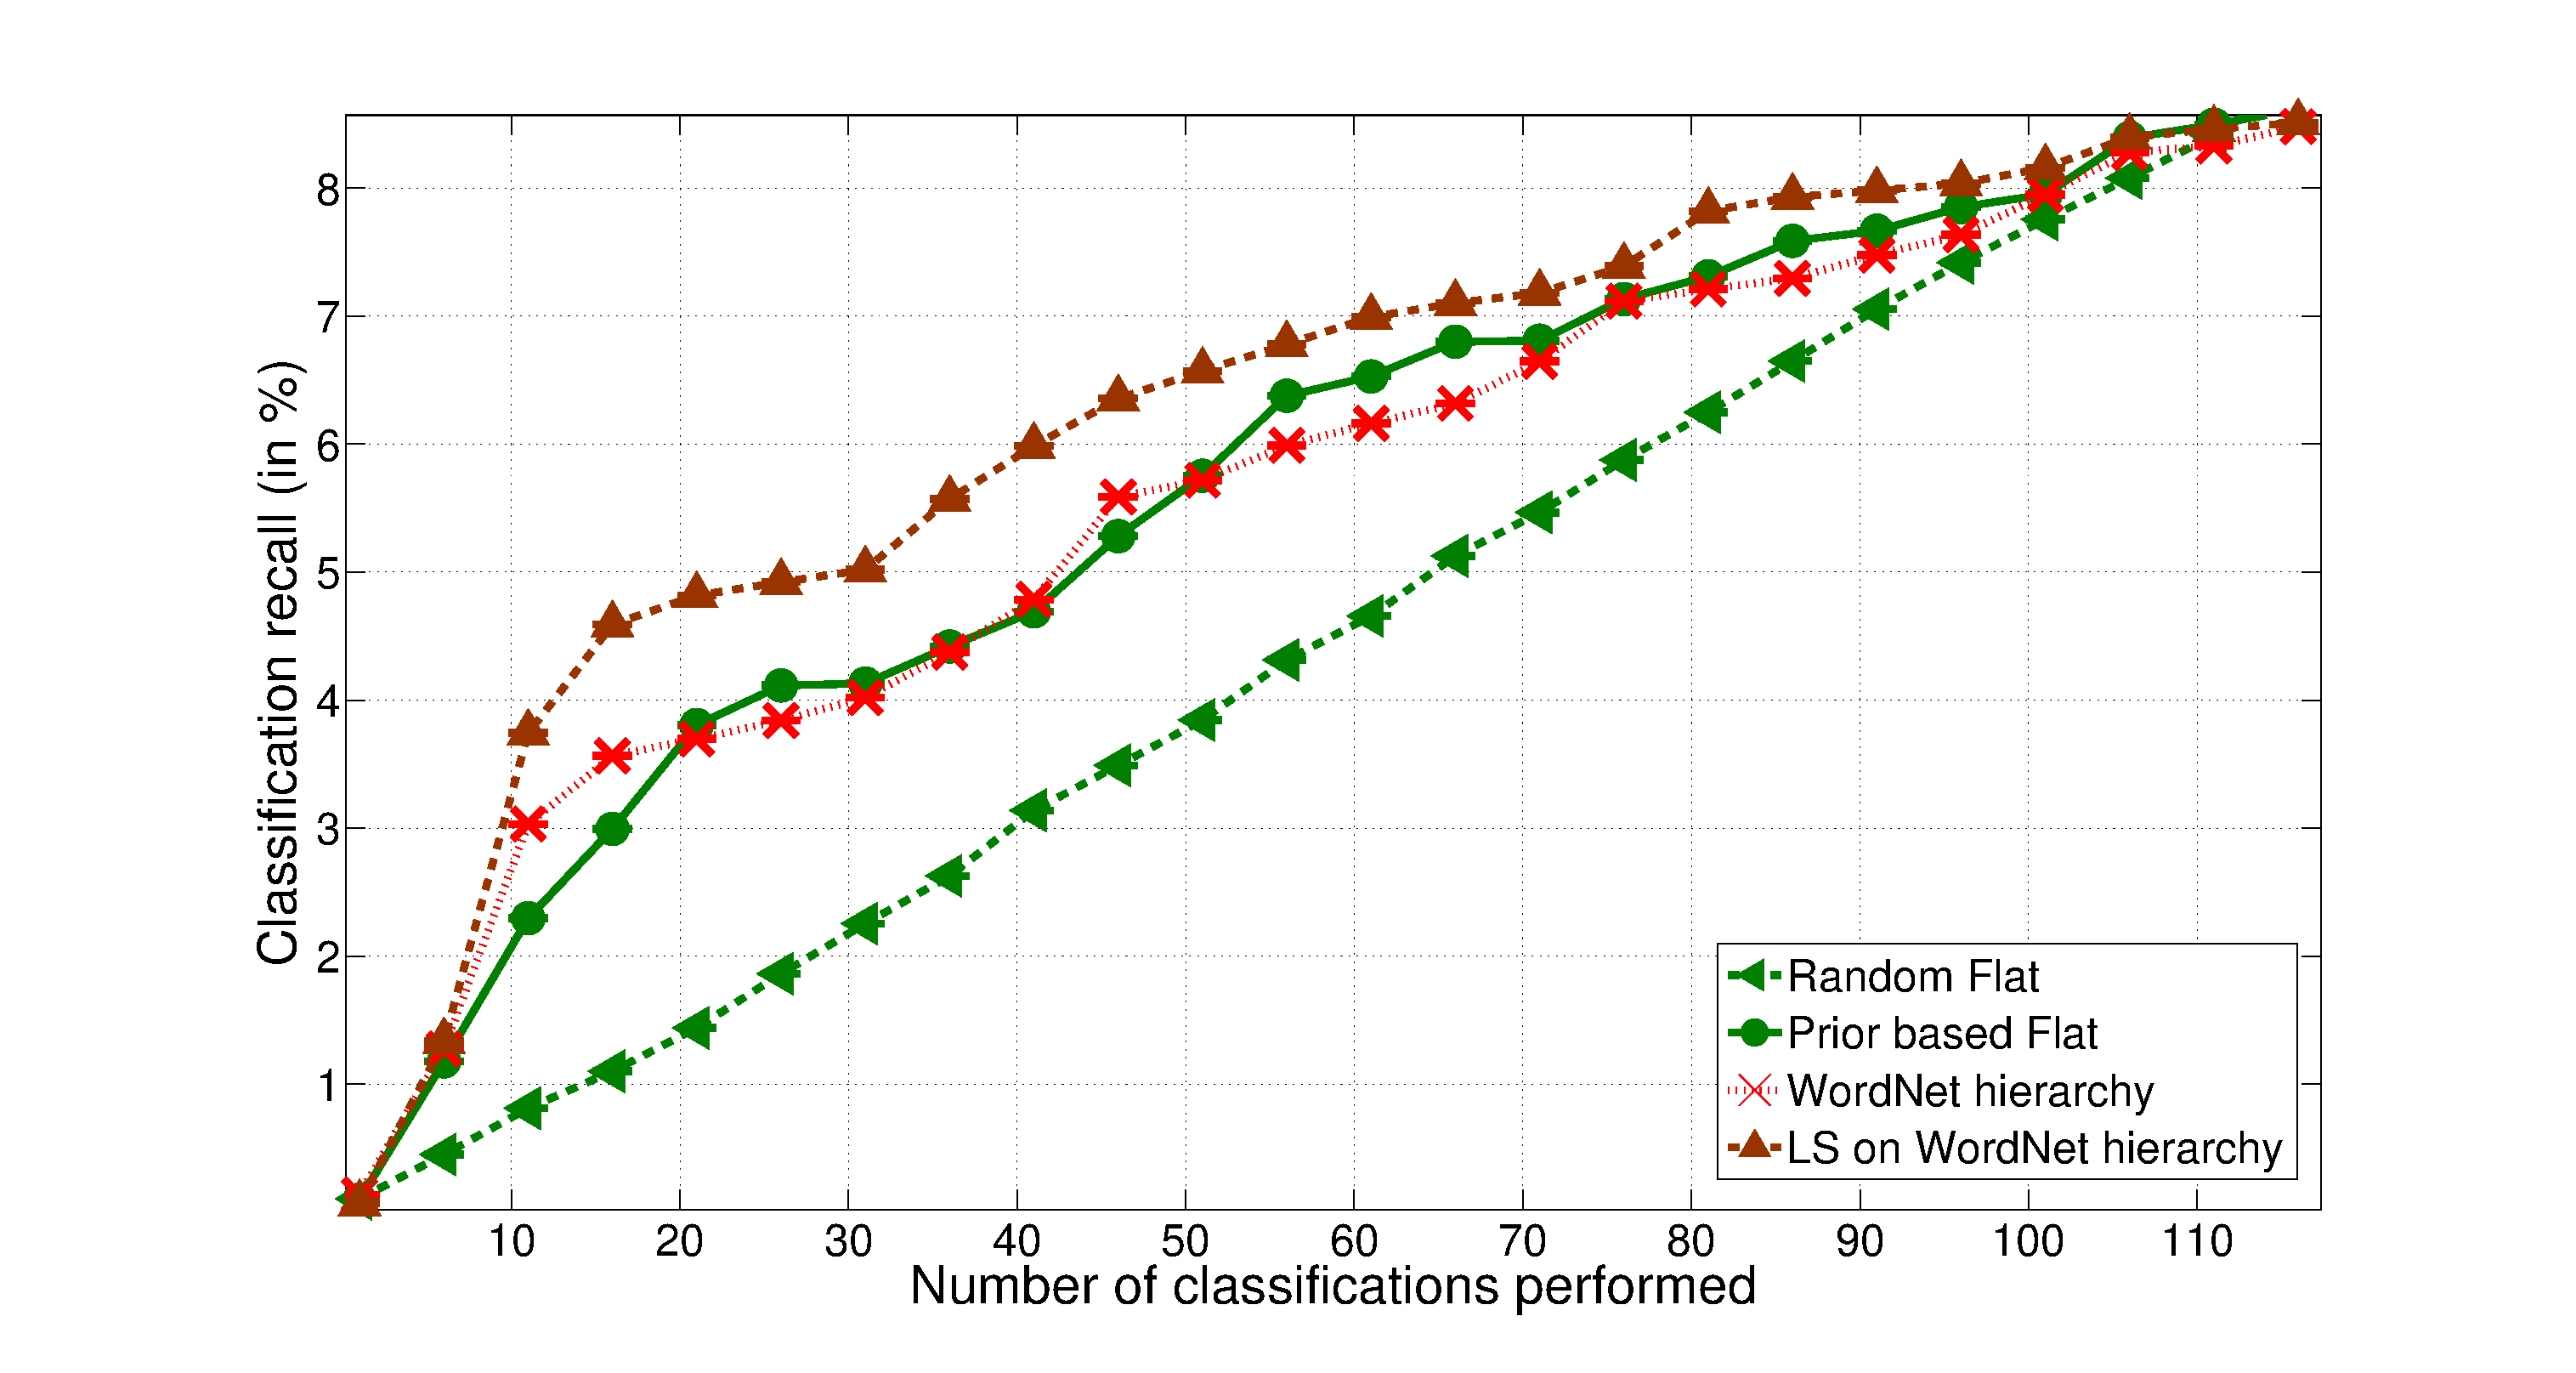
\includegraphics[width=\linewidth]{FastTagPredFWS117topK}
%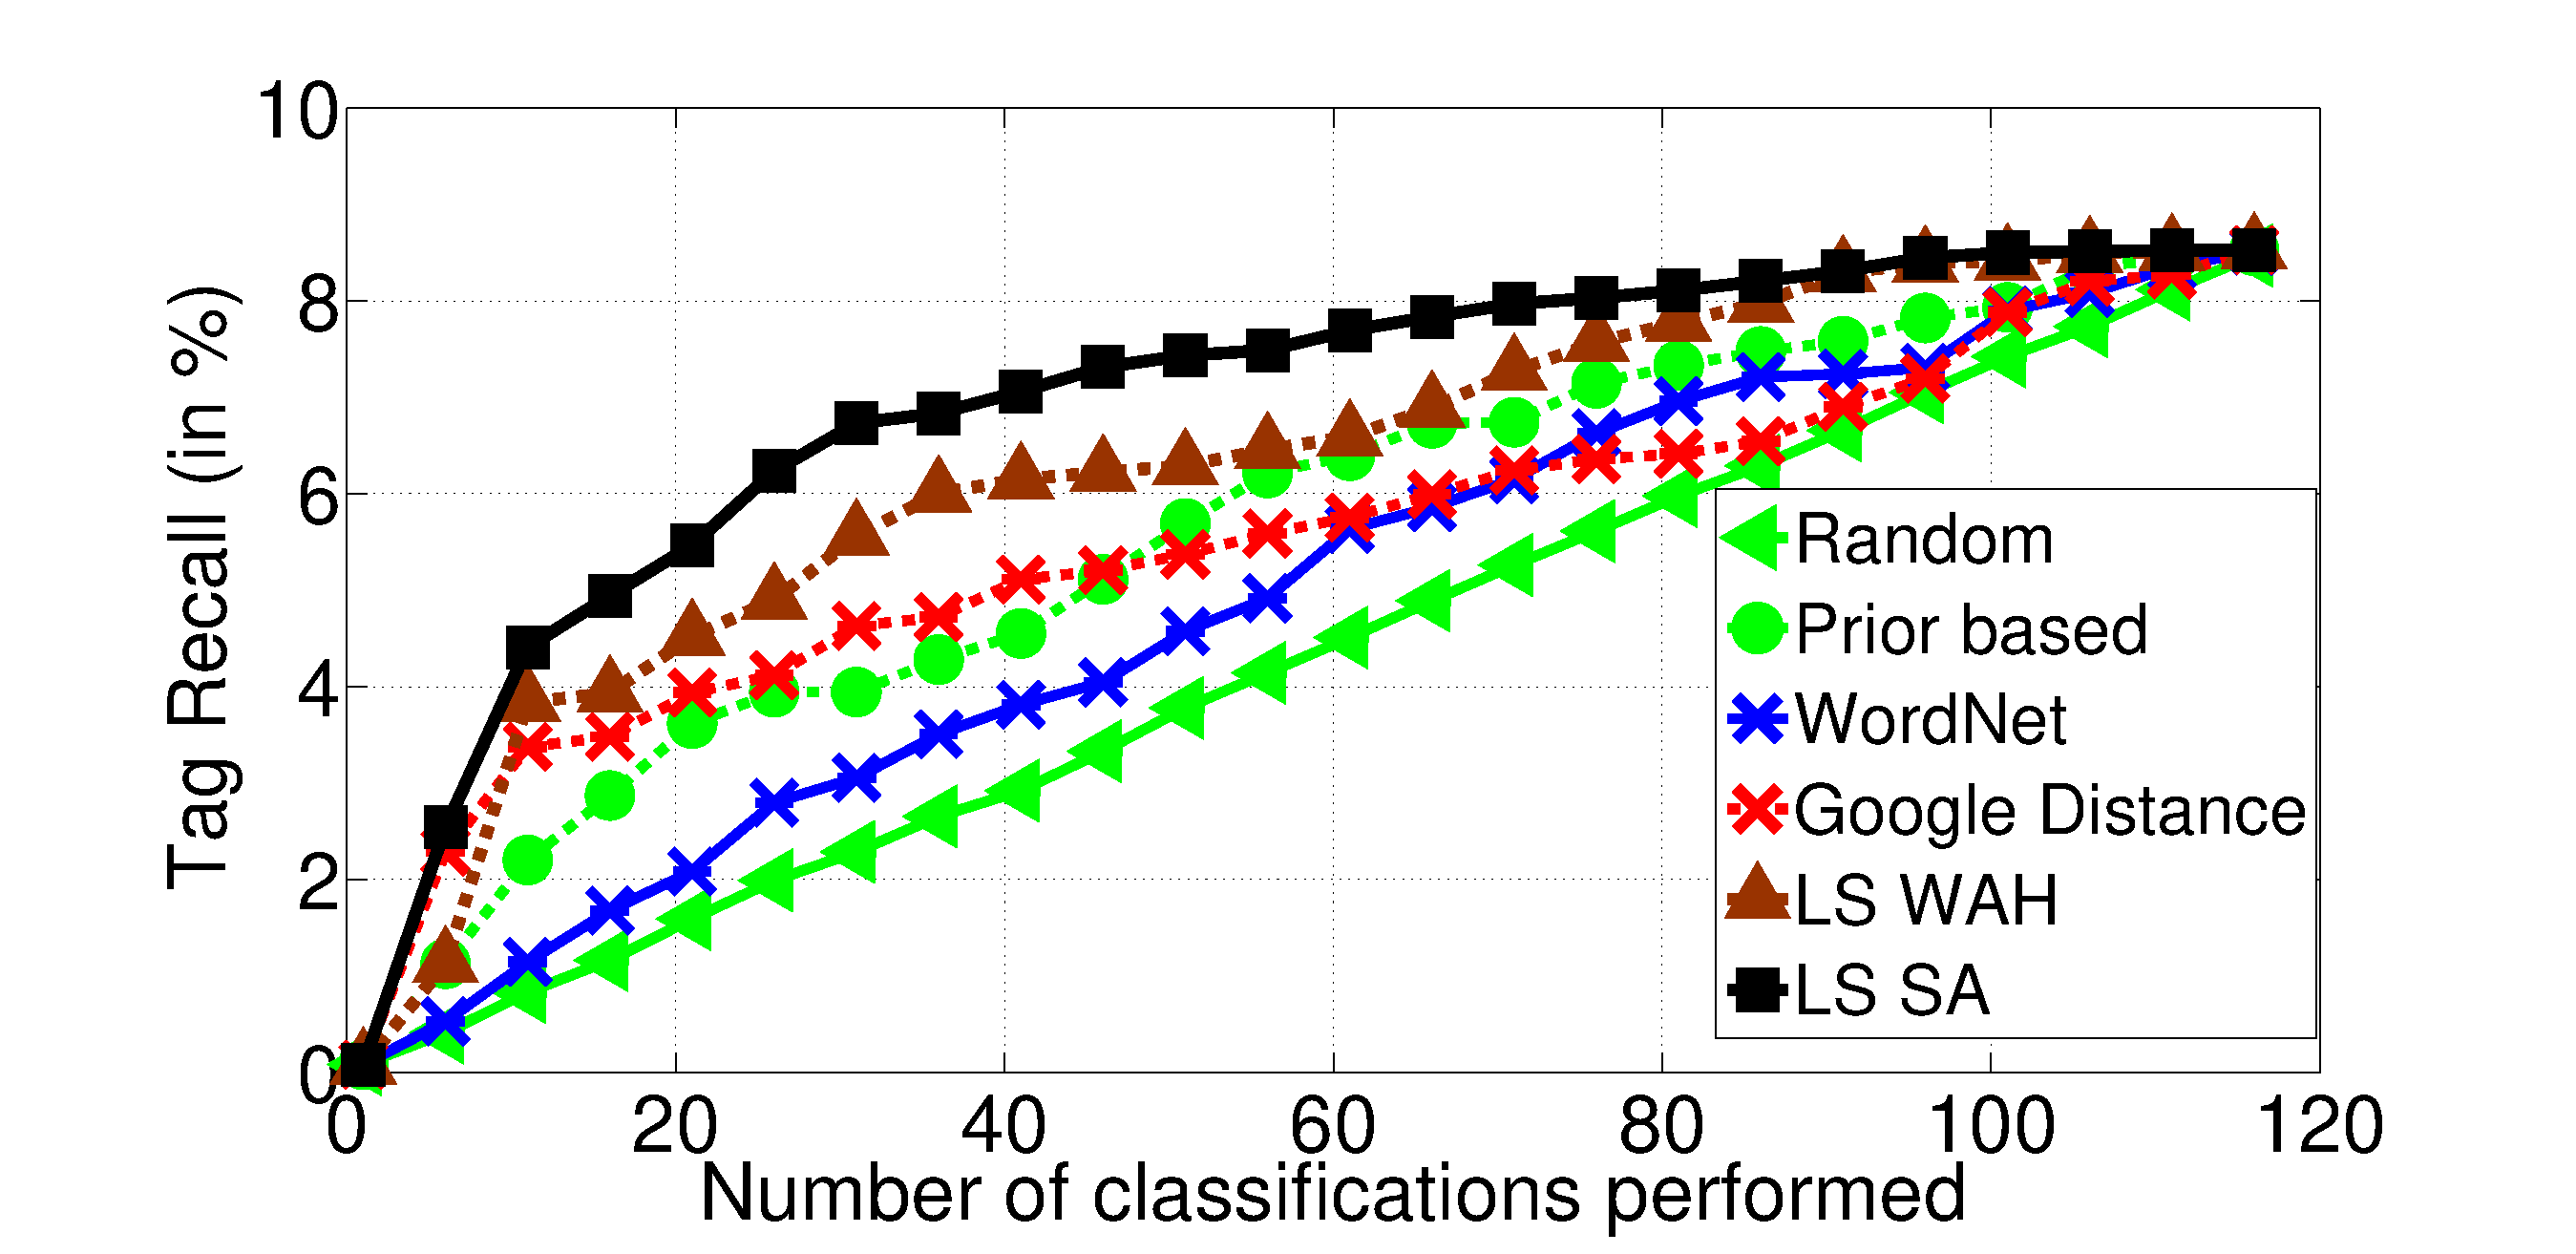
\includegraphics[width=\linewidth]{FWSFastTP_journal.eps}
\centering
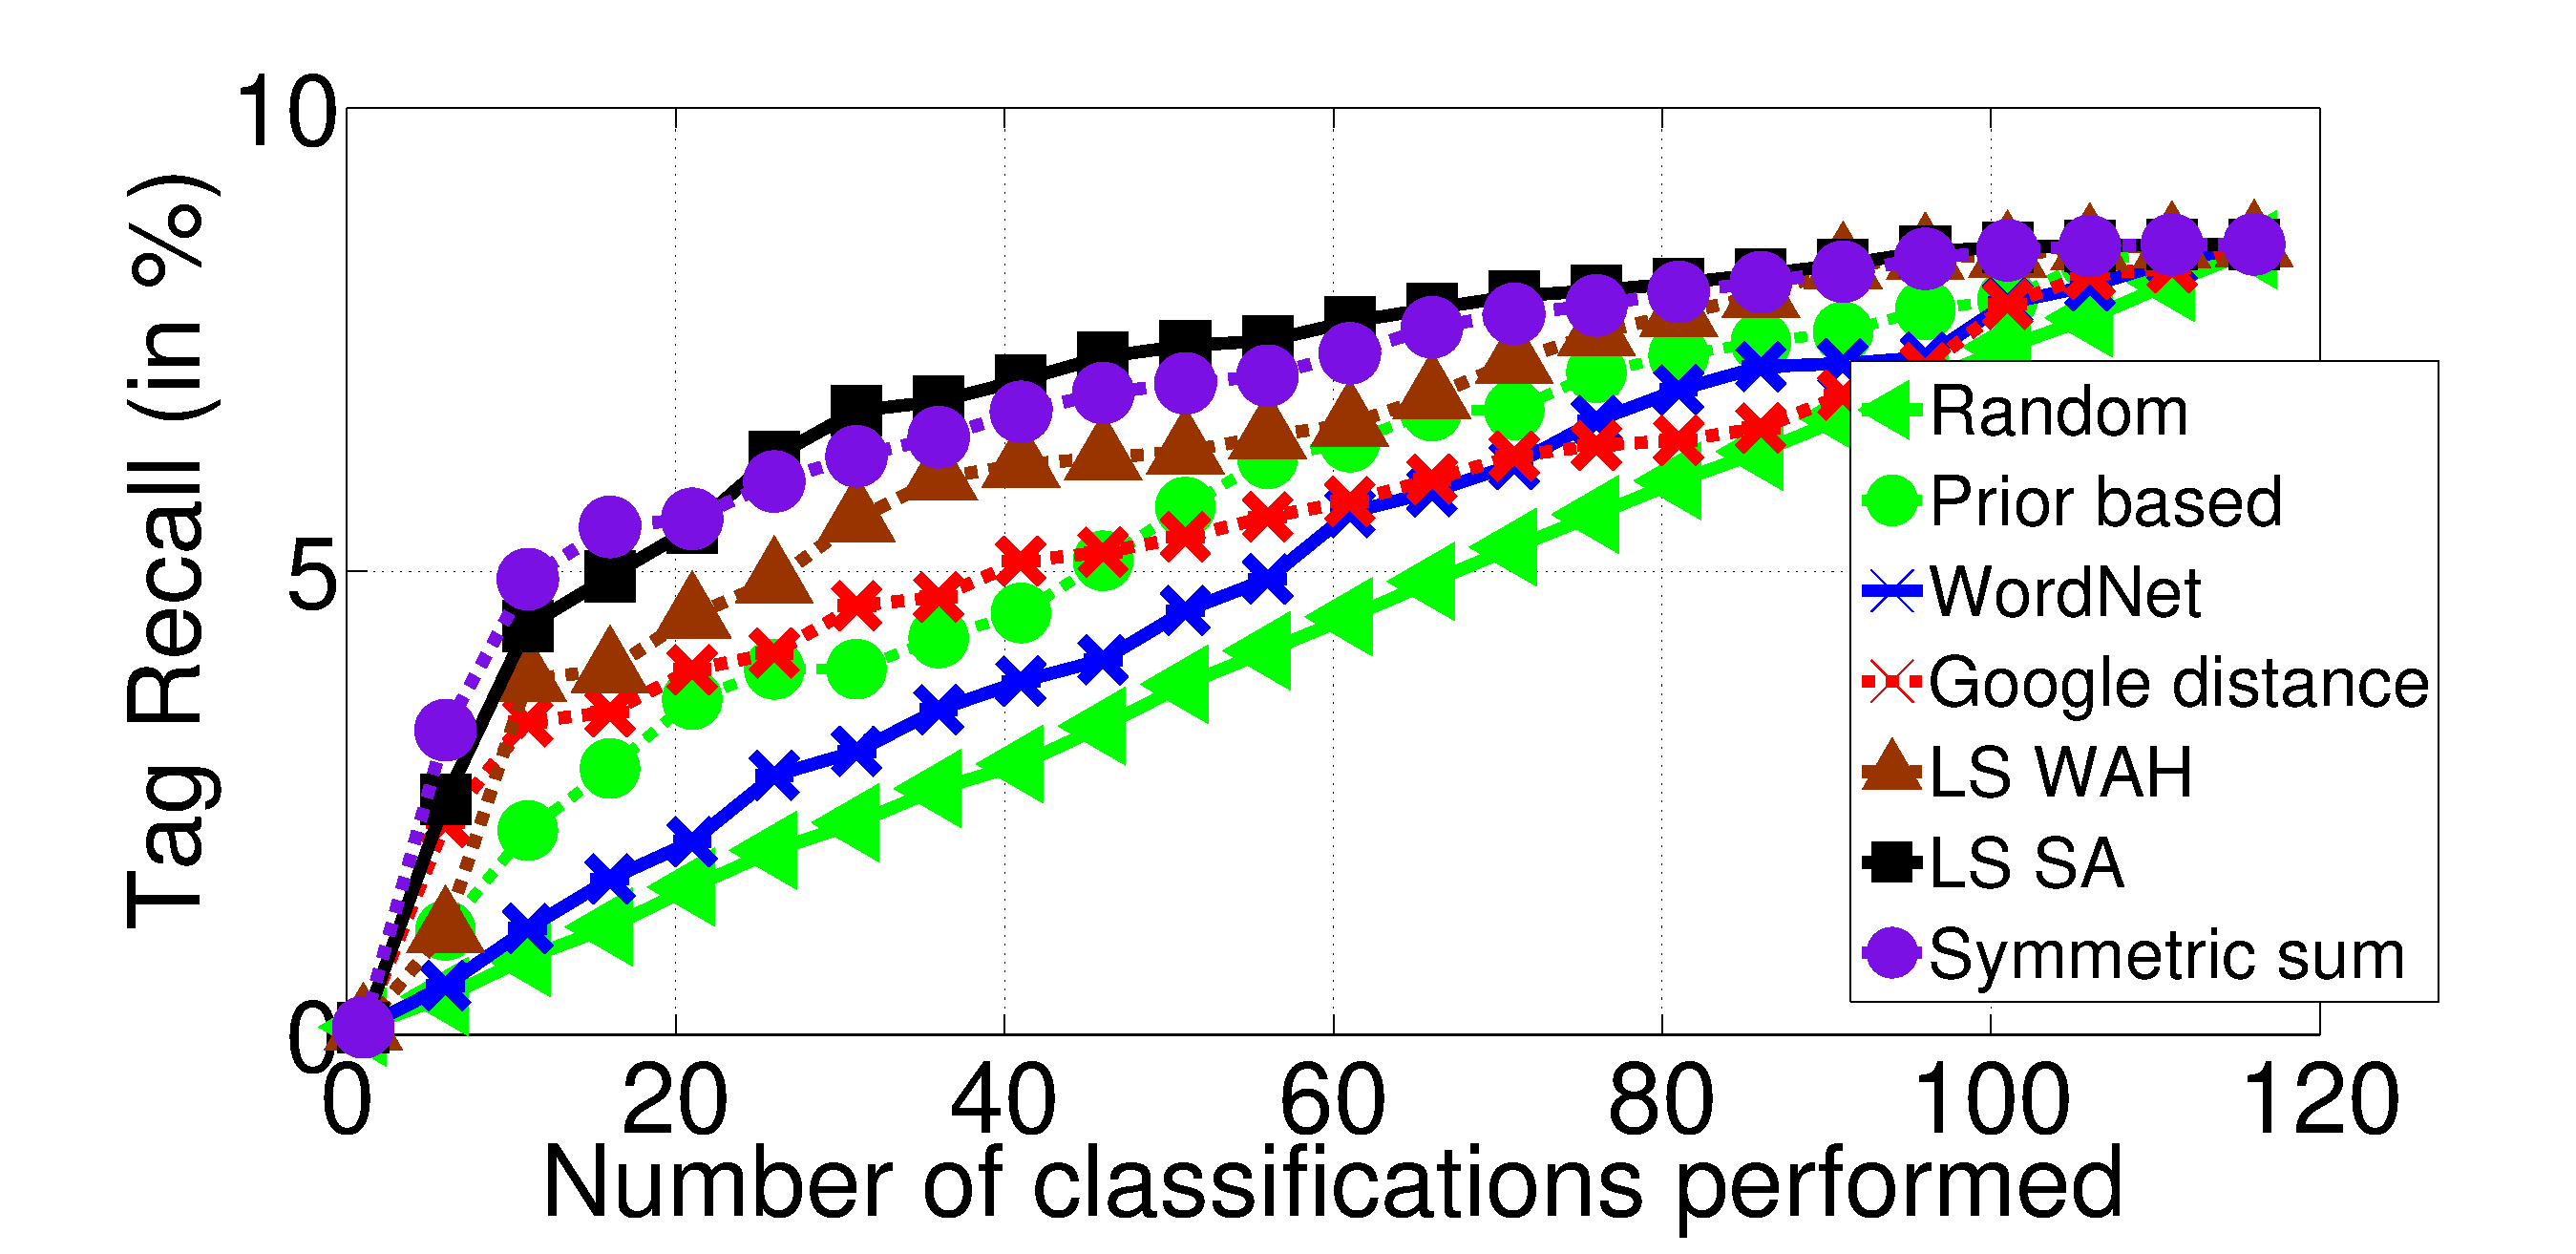
\includegraphics[width=0.65\linewidth]{TagTree/RebuttalFlickrFastTP}
\caption{\hl{Tag Recall obtained with respect to number of classifications performed for Flickr corpus. $\theta$ is chosen to  be 0.5.} } 
\label{fig:EfficientTagPredGraphFlickr}
\end{figure}
\begin{figure}[!htp]
%\epsfig{width=10cm,figure=FastTagPredFWS117topK.eps}
%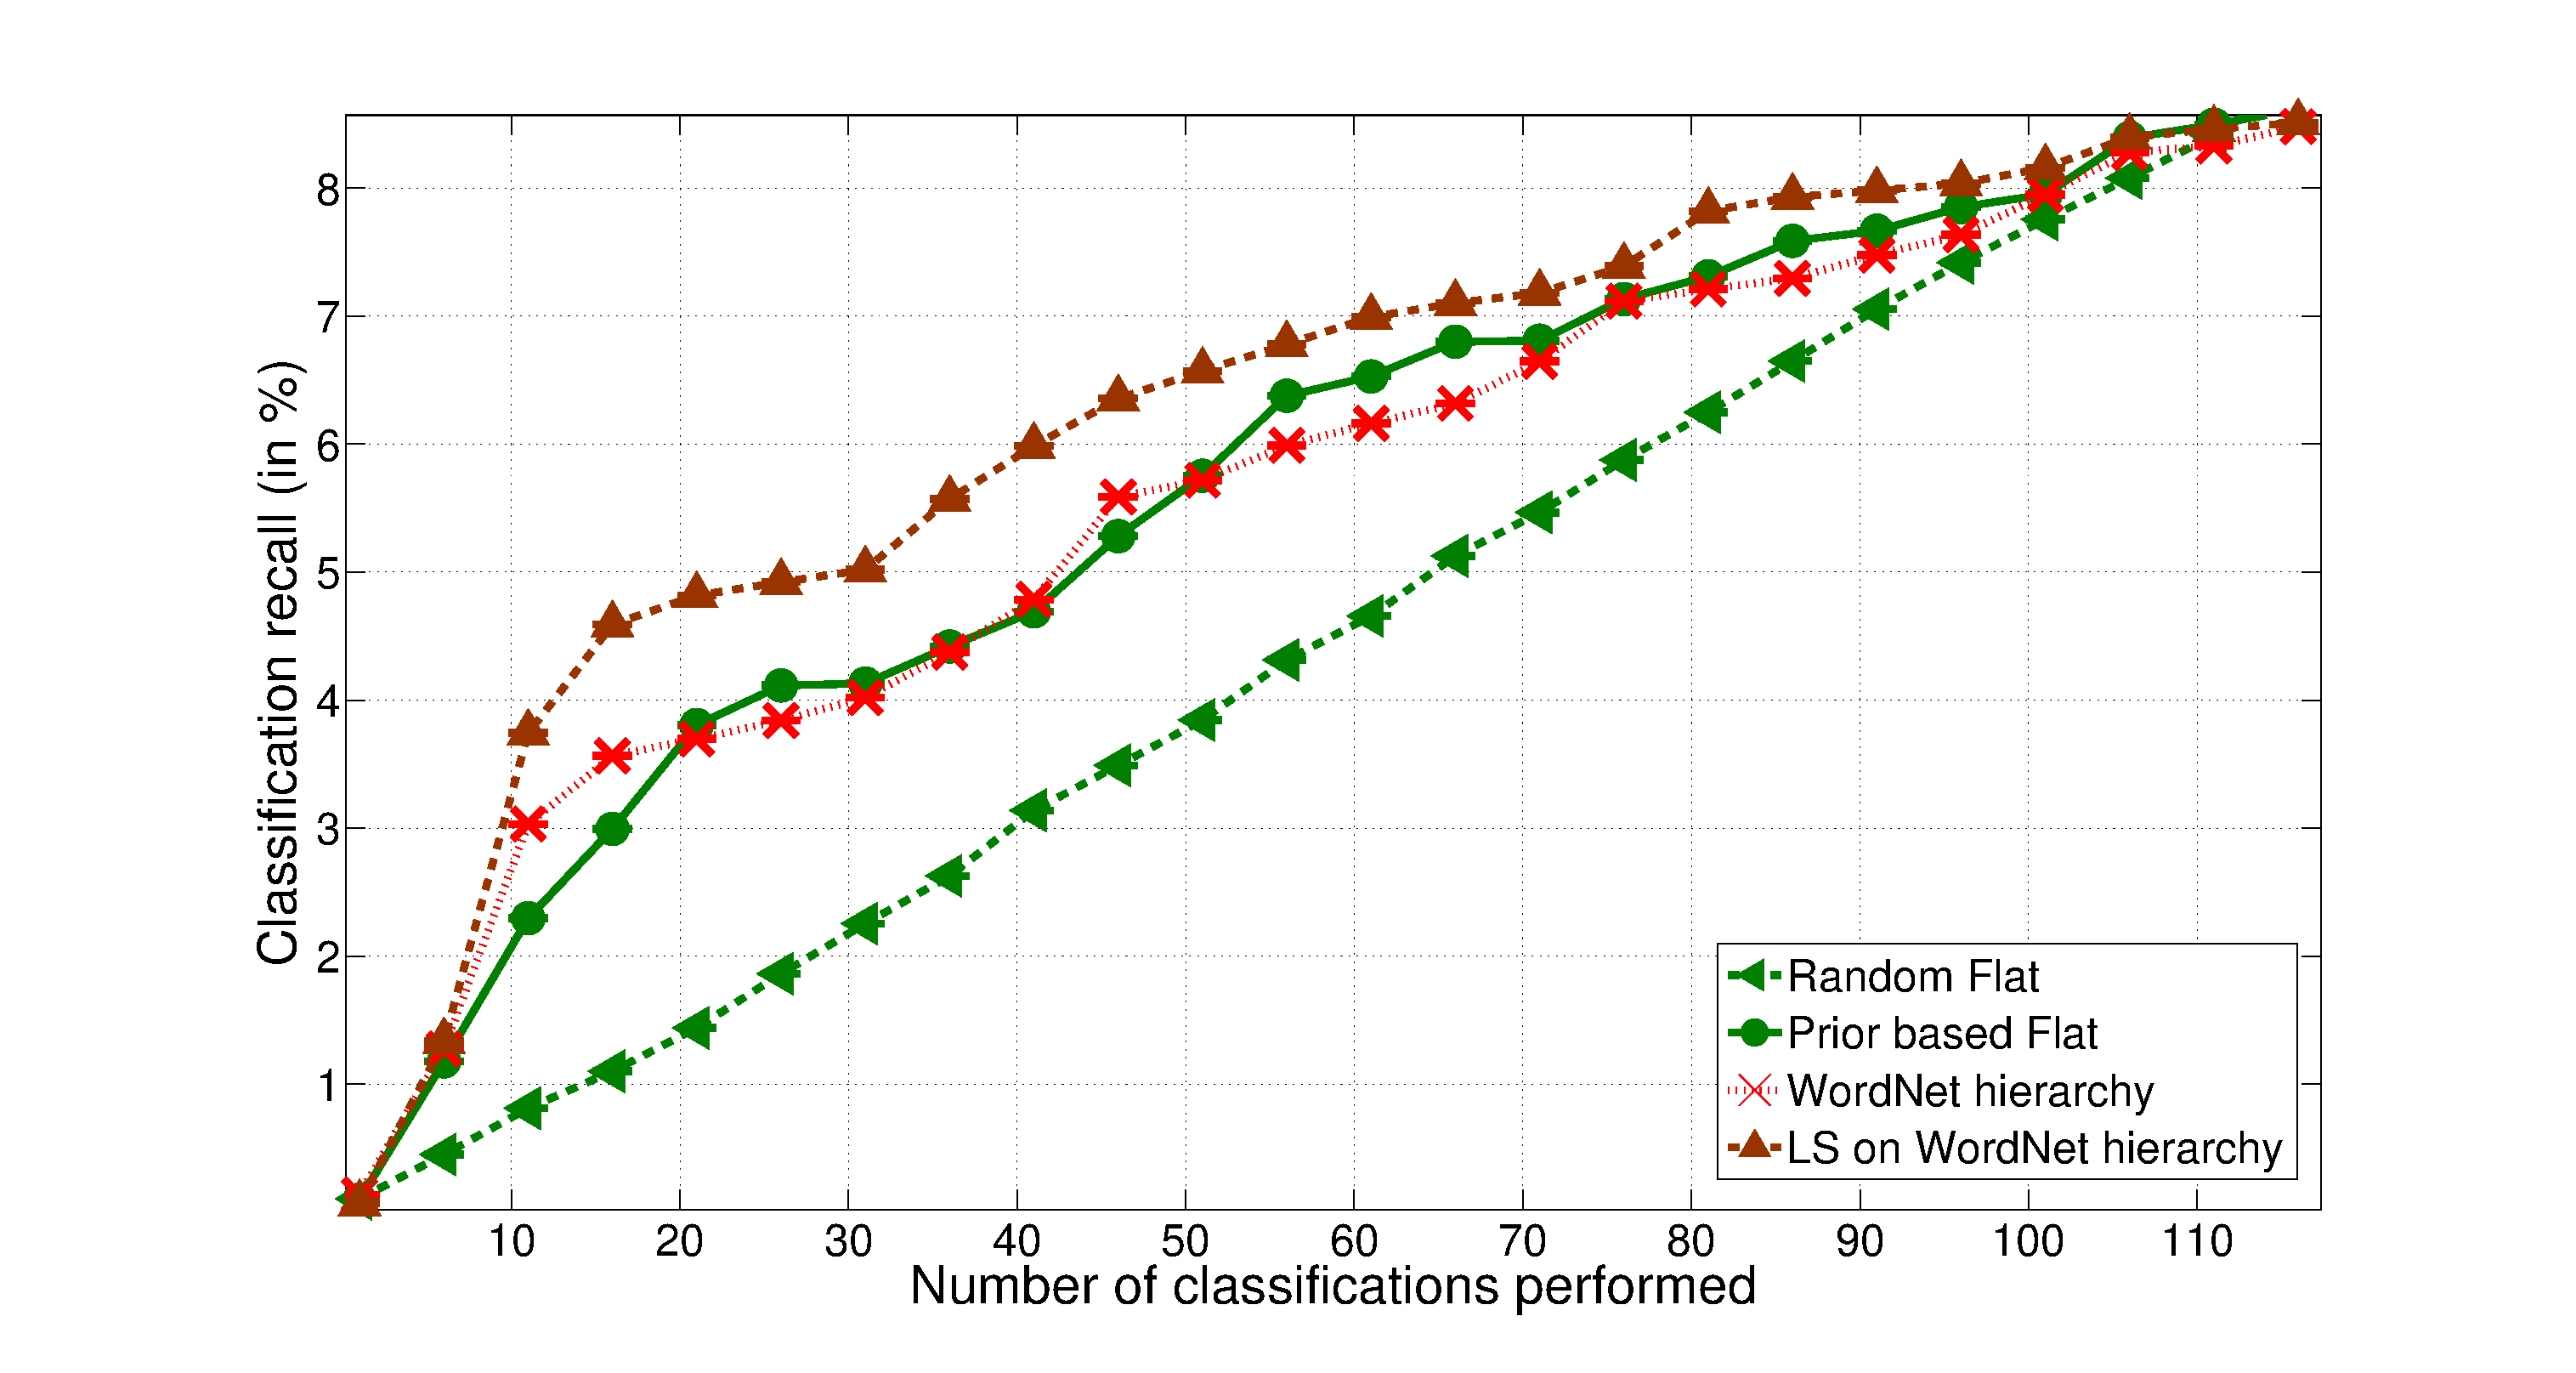
\includegraphics[width=\linewidth]{FastTagPredFWS117topK}
%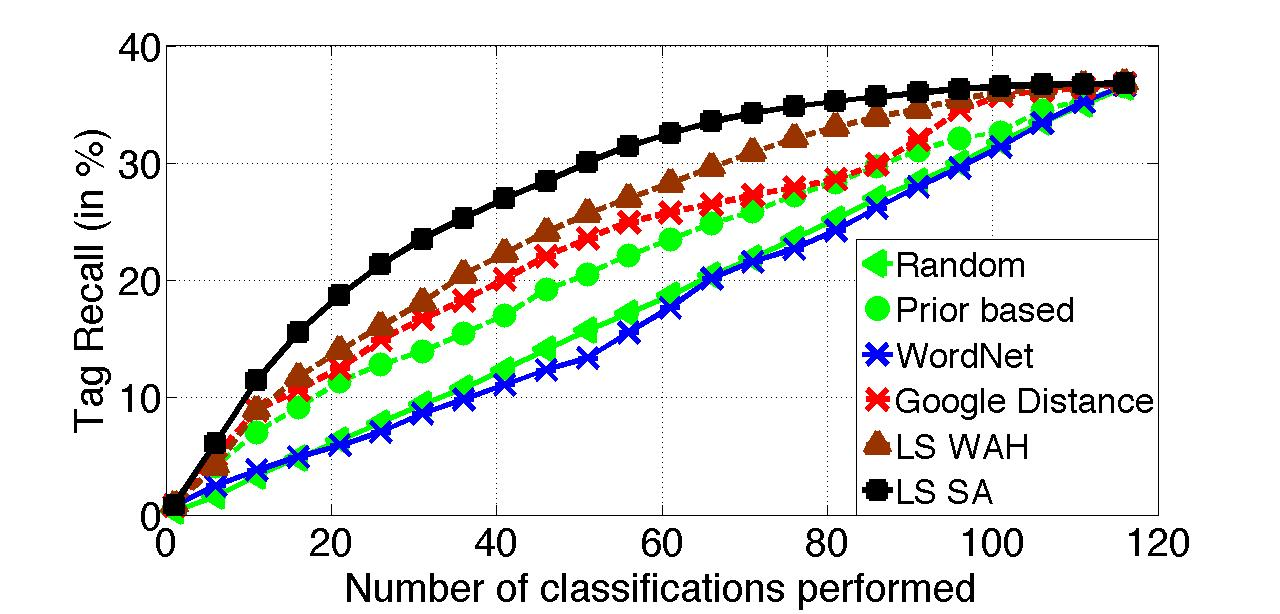
\includegraphics[width=\linewidth]{Journal_FastTagPredResults_LowerThreshMinpt5}
\centering
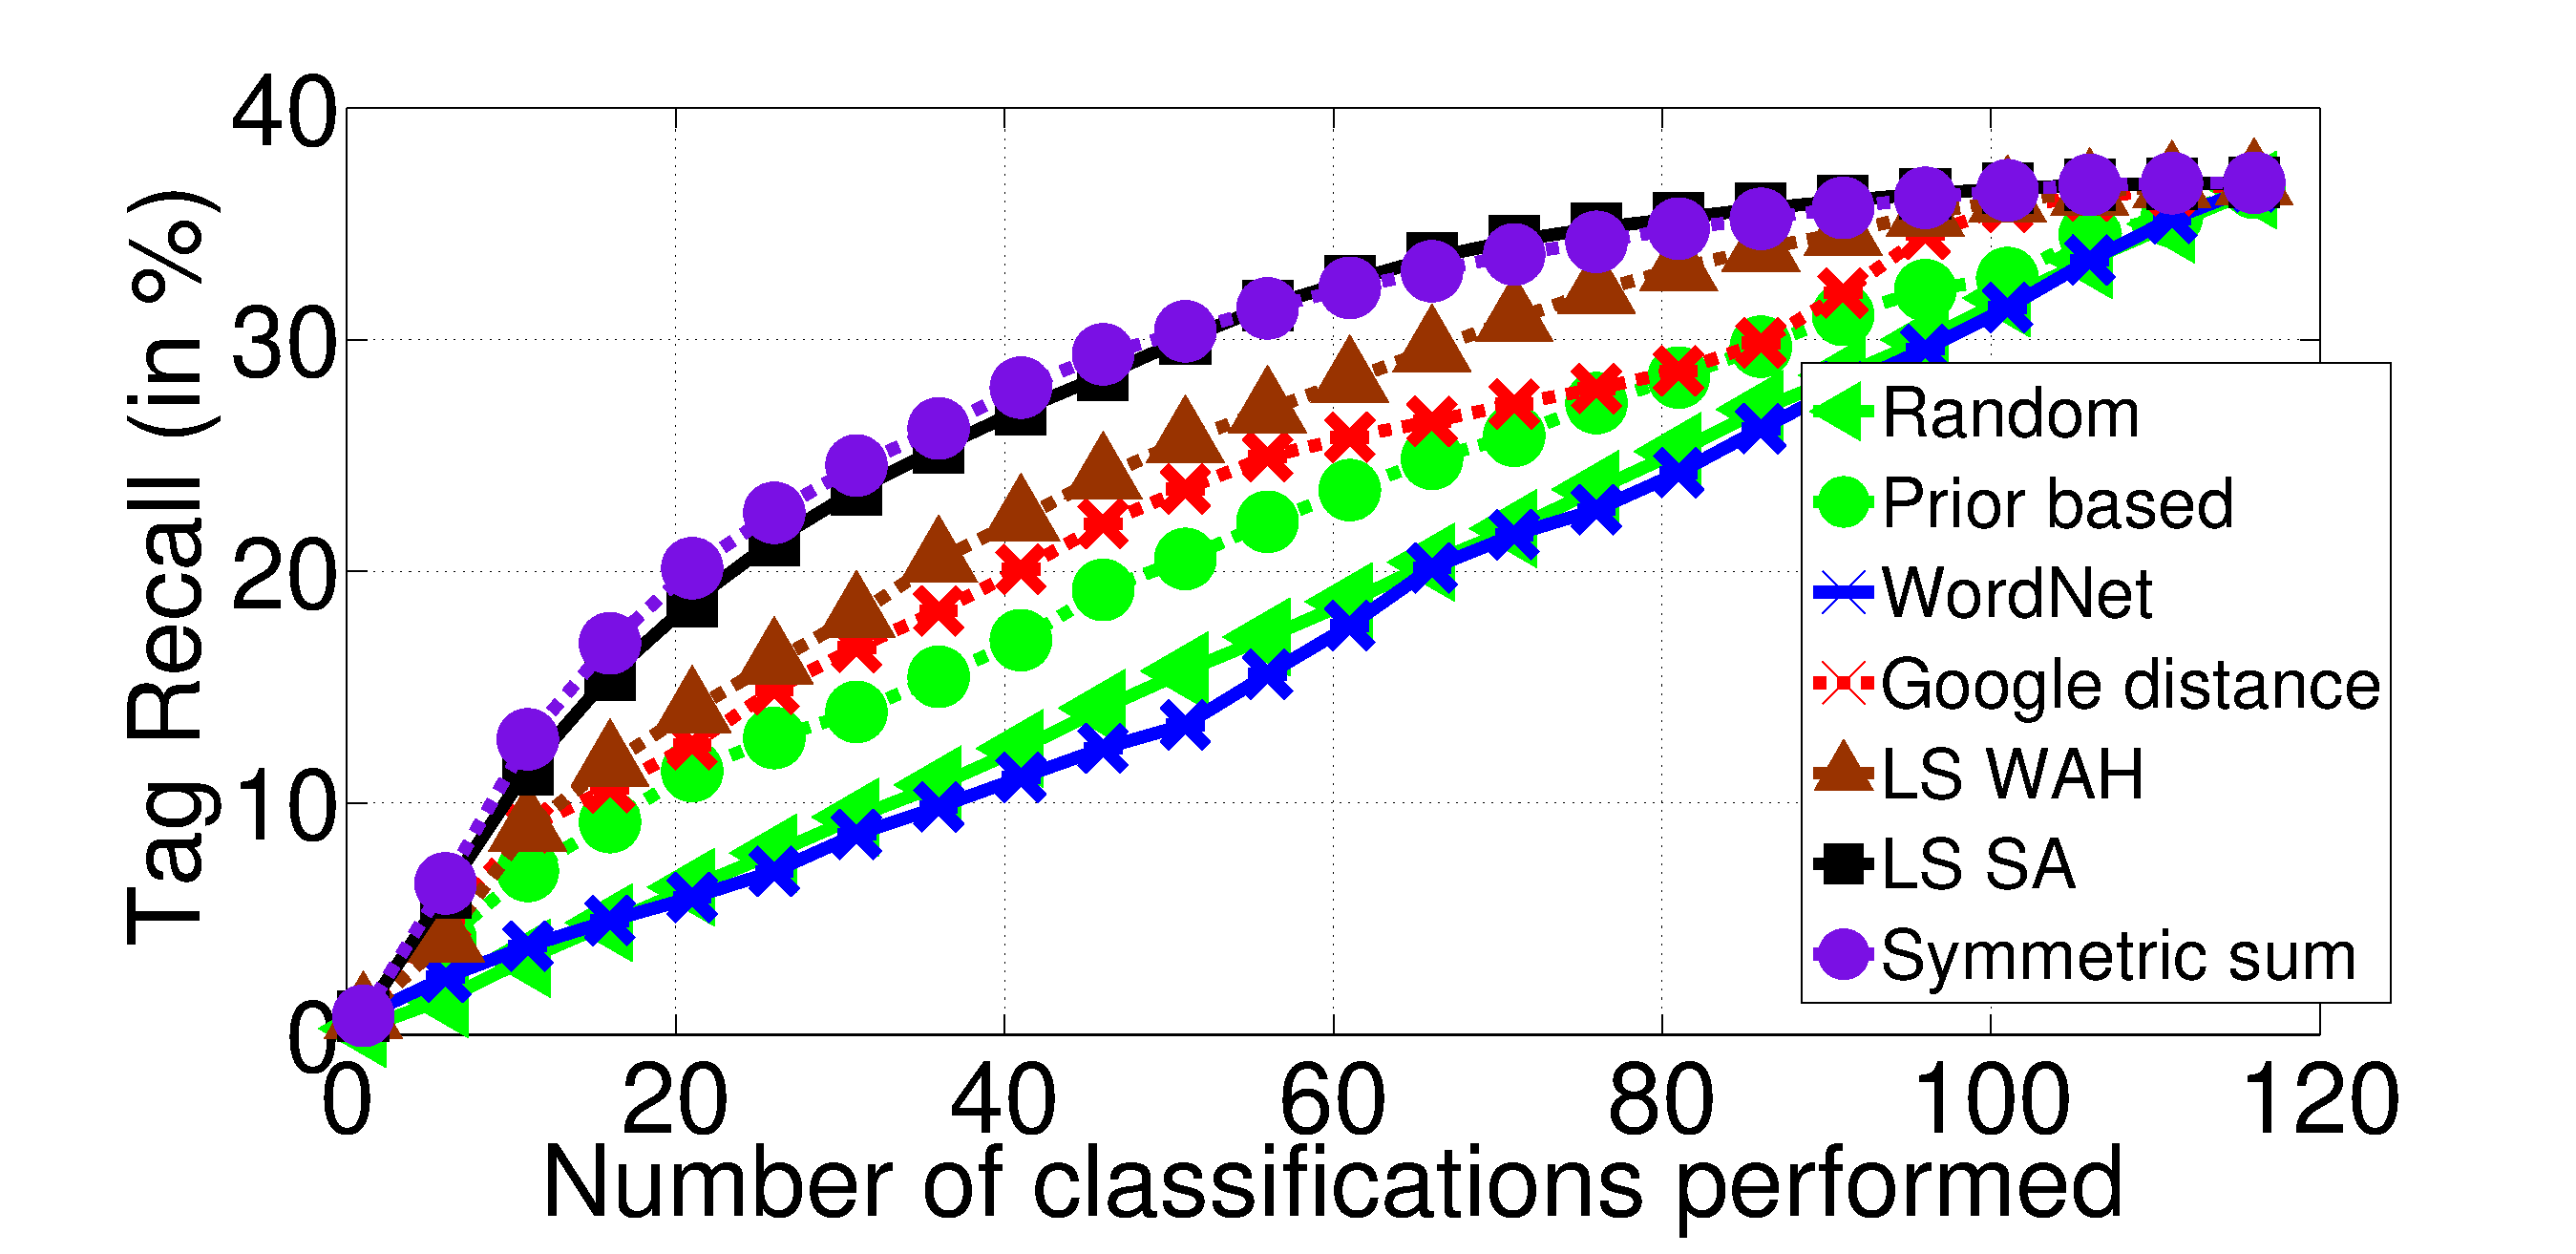
\includegraphics[width=0.65\linewidth]{TagTree/Rebuttal_FWS_Fast_LOWER}
\caption{\hl{Tag Recall obtained with respect to number of classifications performed for Flickr corpus. $\theta$ is chosen to be 0.33. } }
\label{fig:EfficientTagPredGraphFlickrLower}
\end{figure}
\begin{figure}[!htp]
%\epsfig{width=10cm,figure=FastTagPredGWS118topK.eps}
%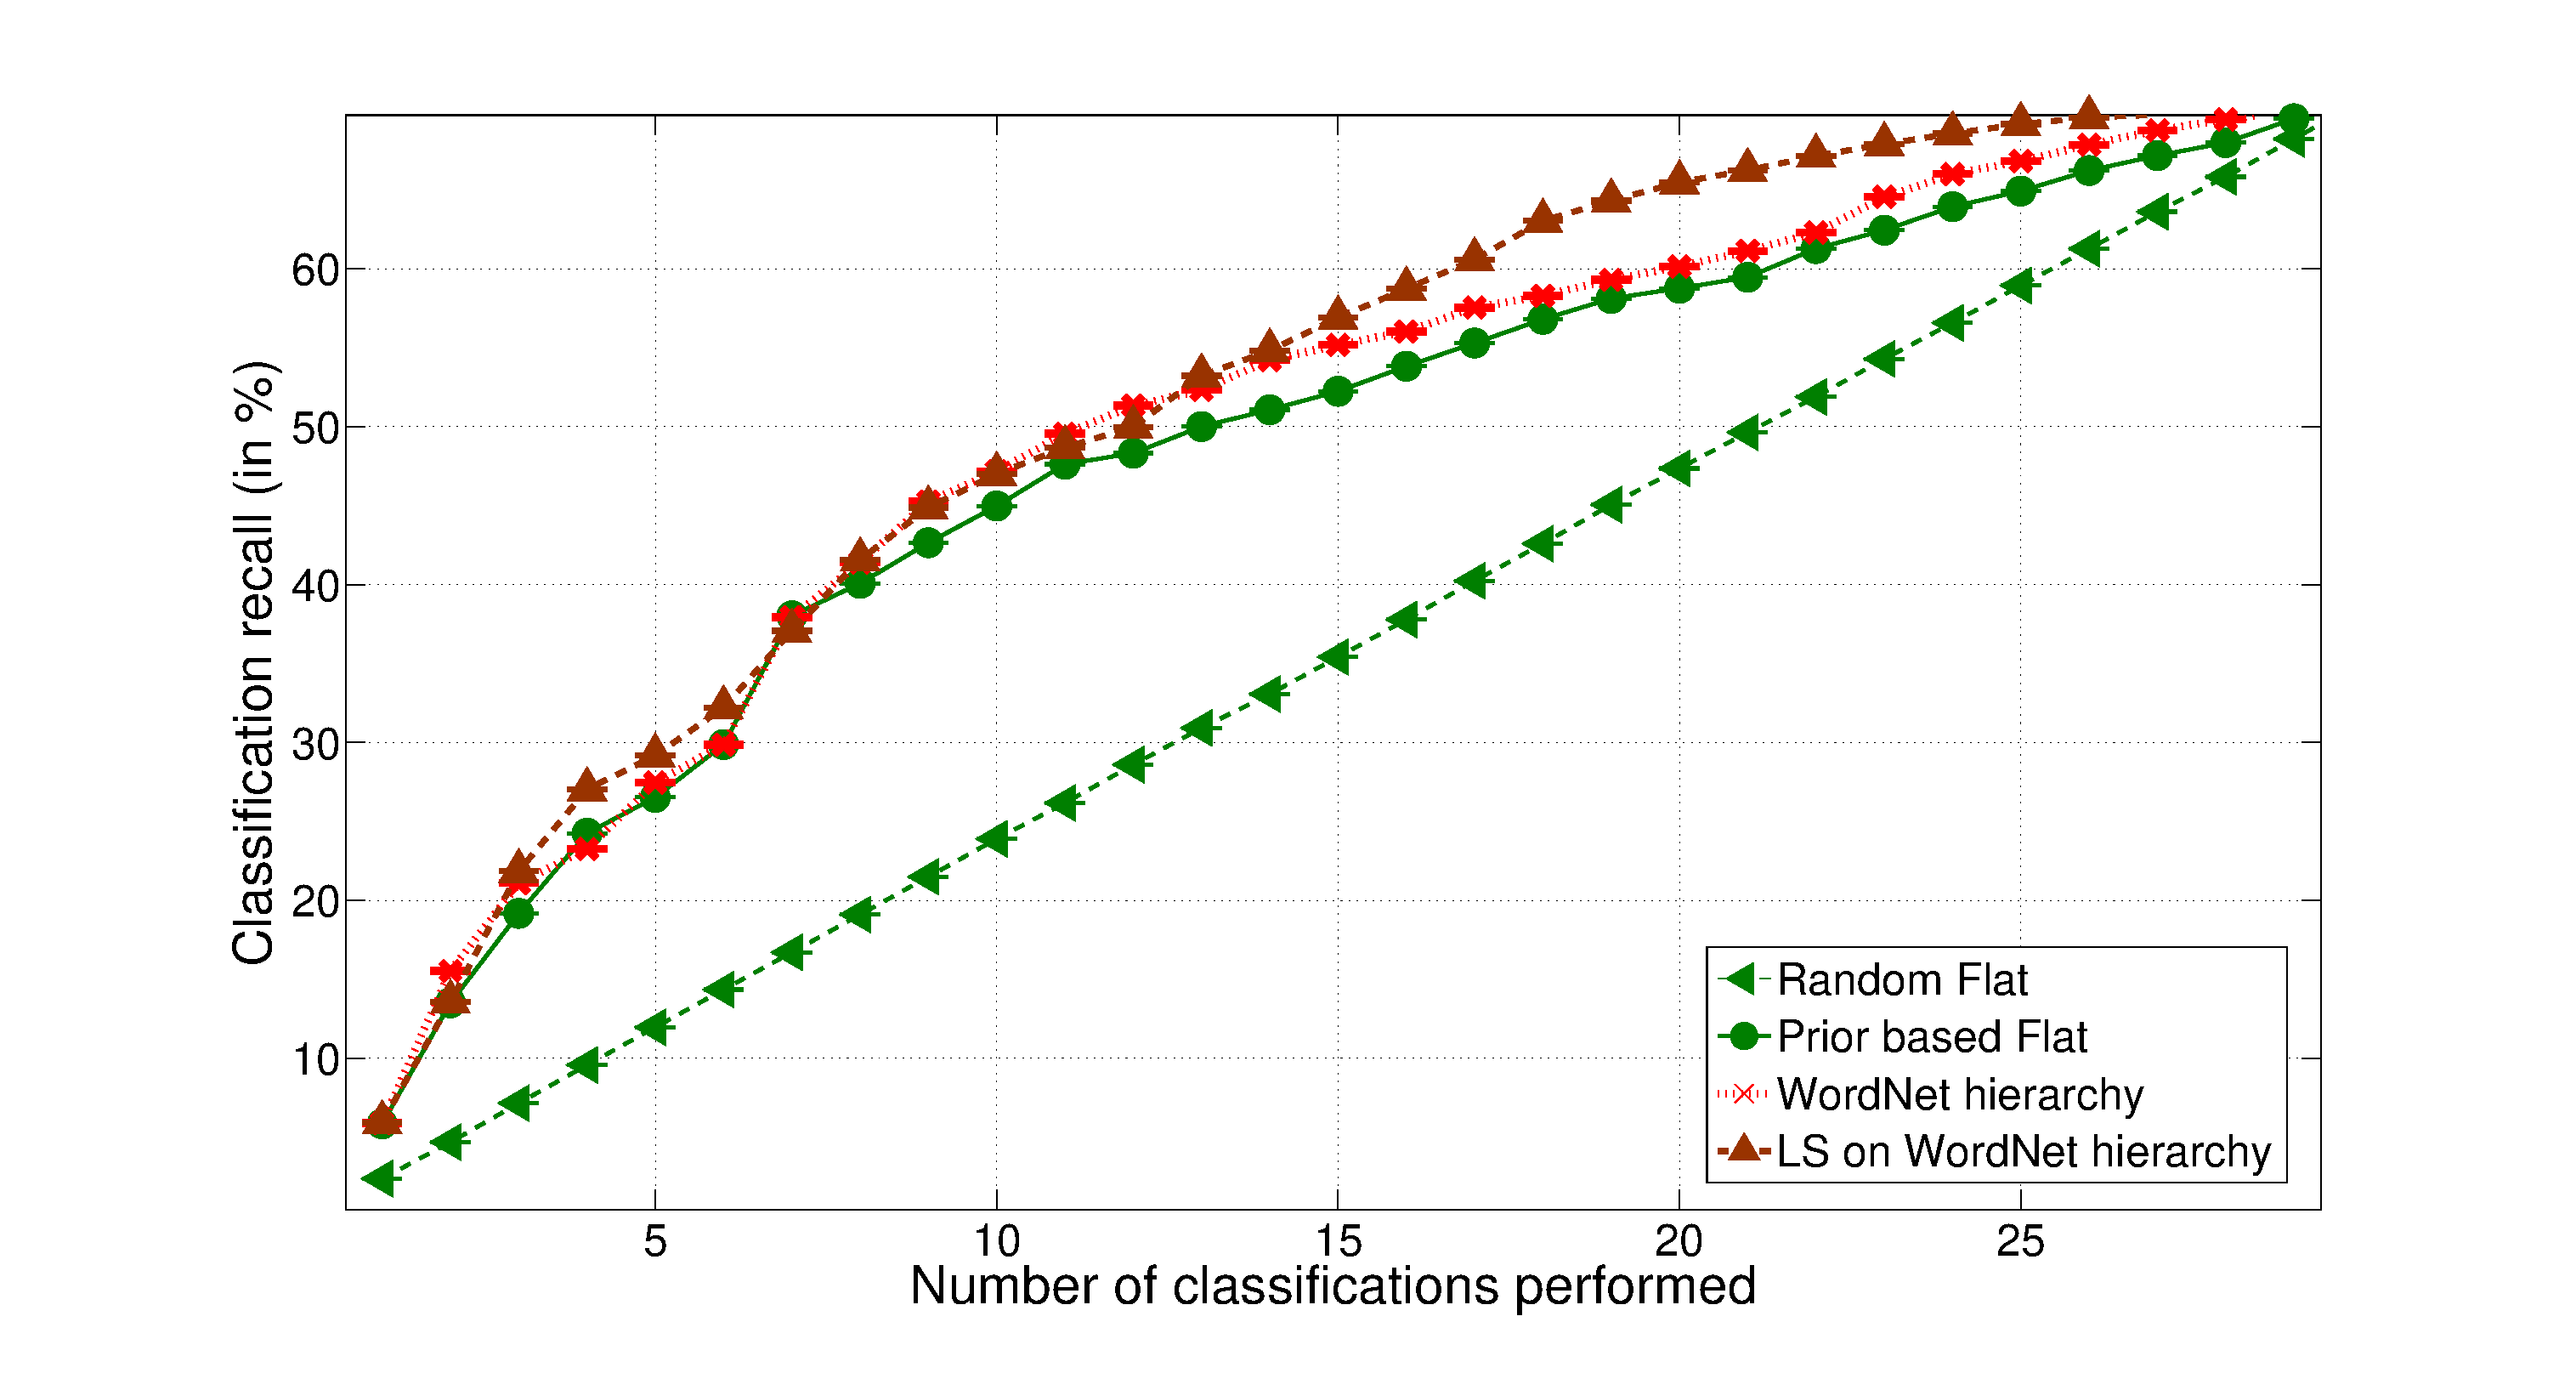
\includegraphics[width=\linewidth]{FastTagPredGWS118topK}
%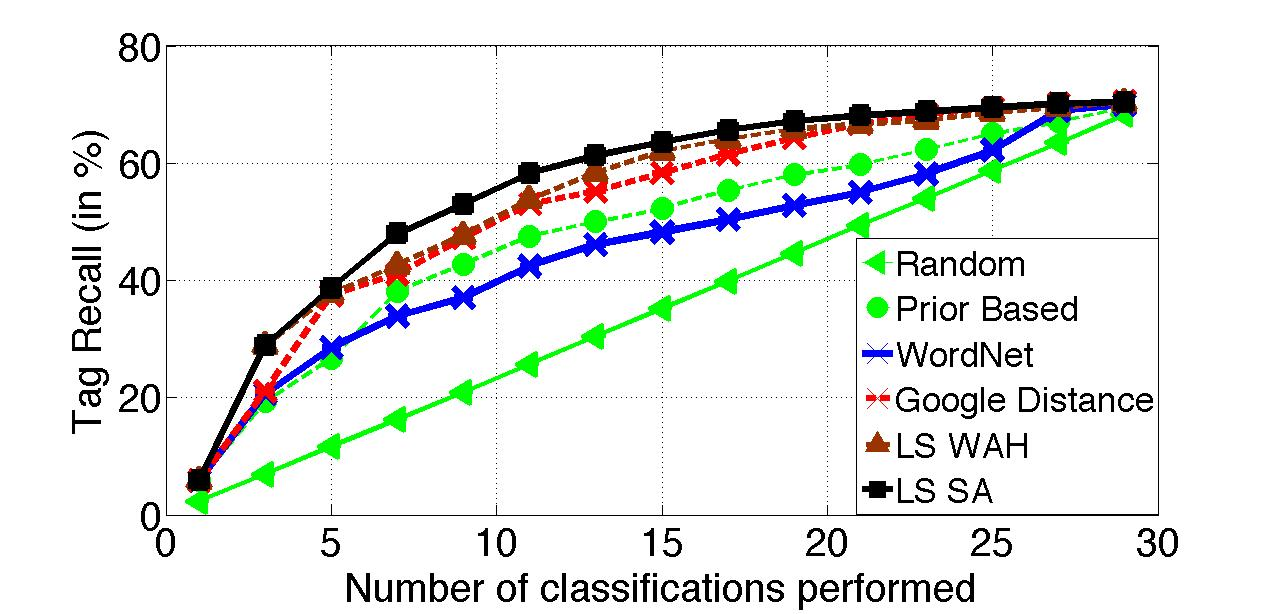
\includegraphics[width=\linewidth]{GWS30_FastTP_journal2}
\centering
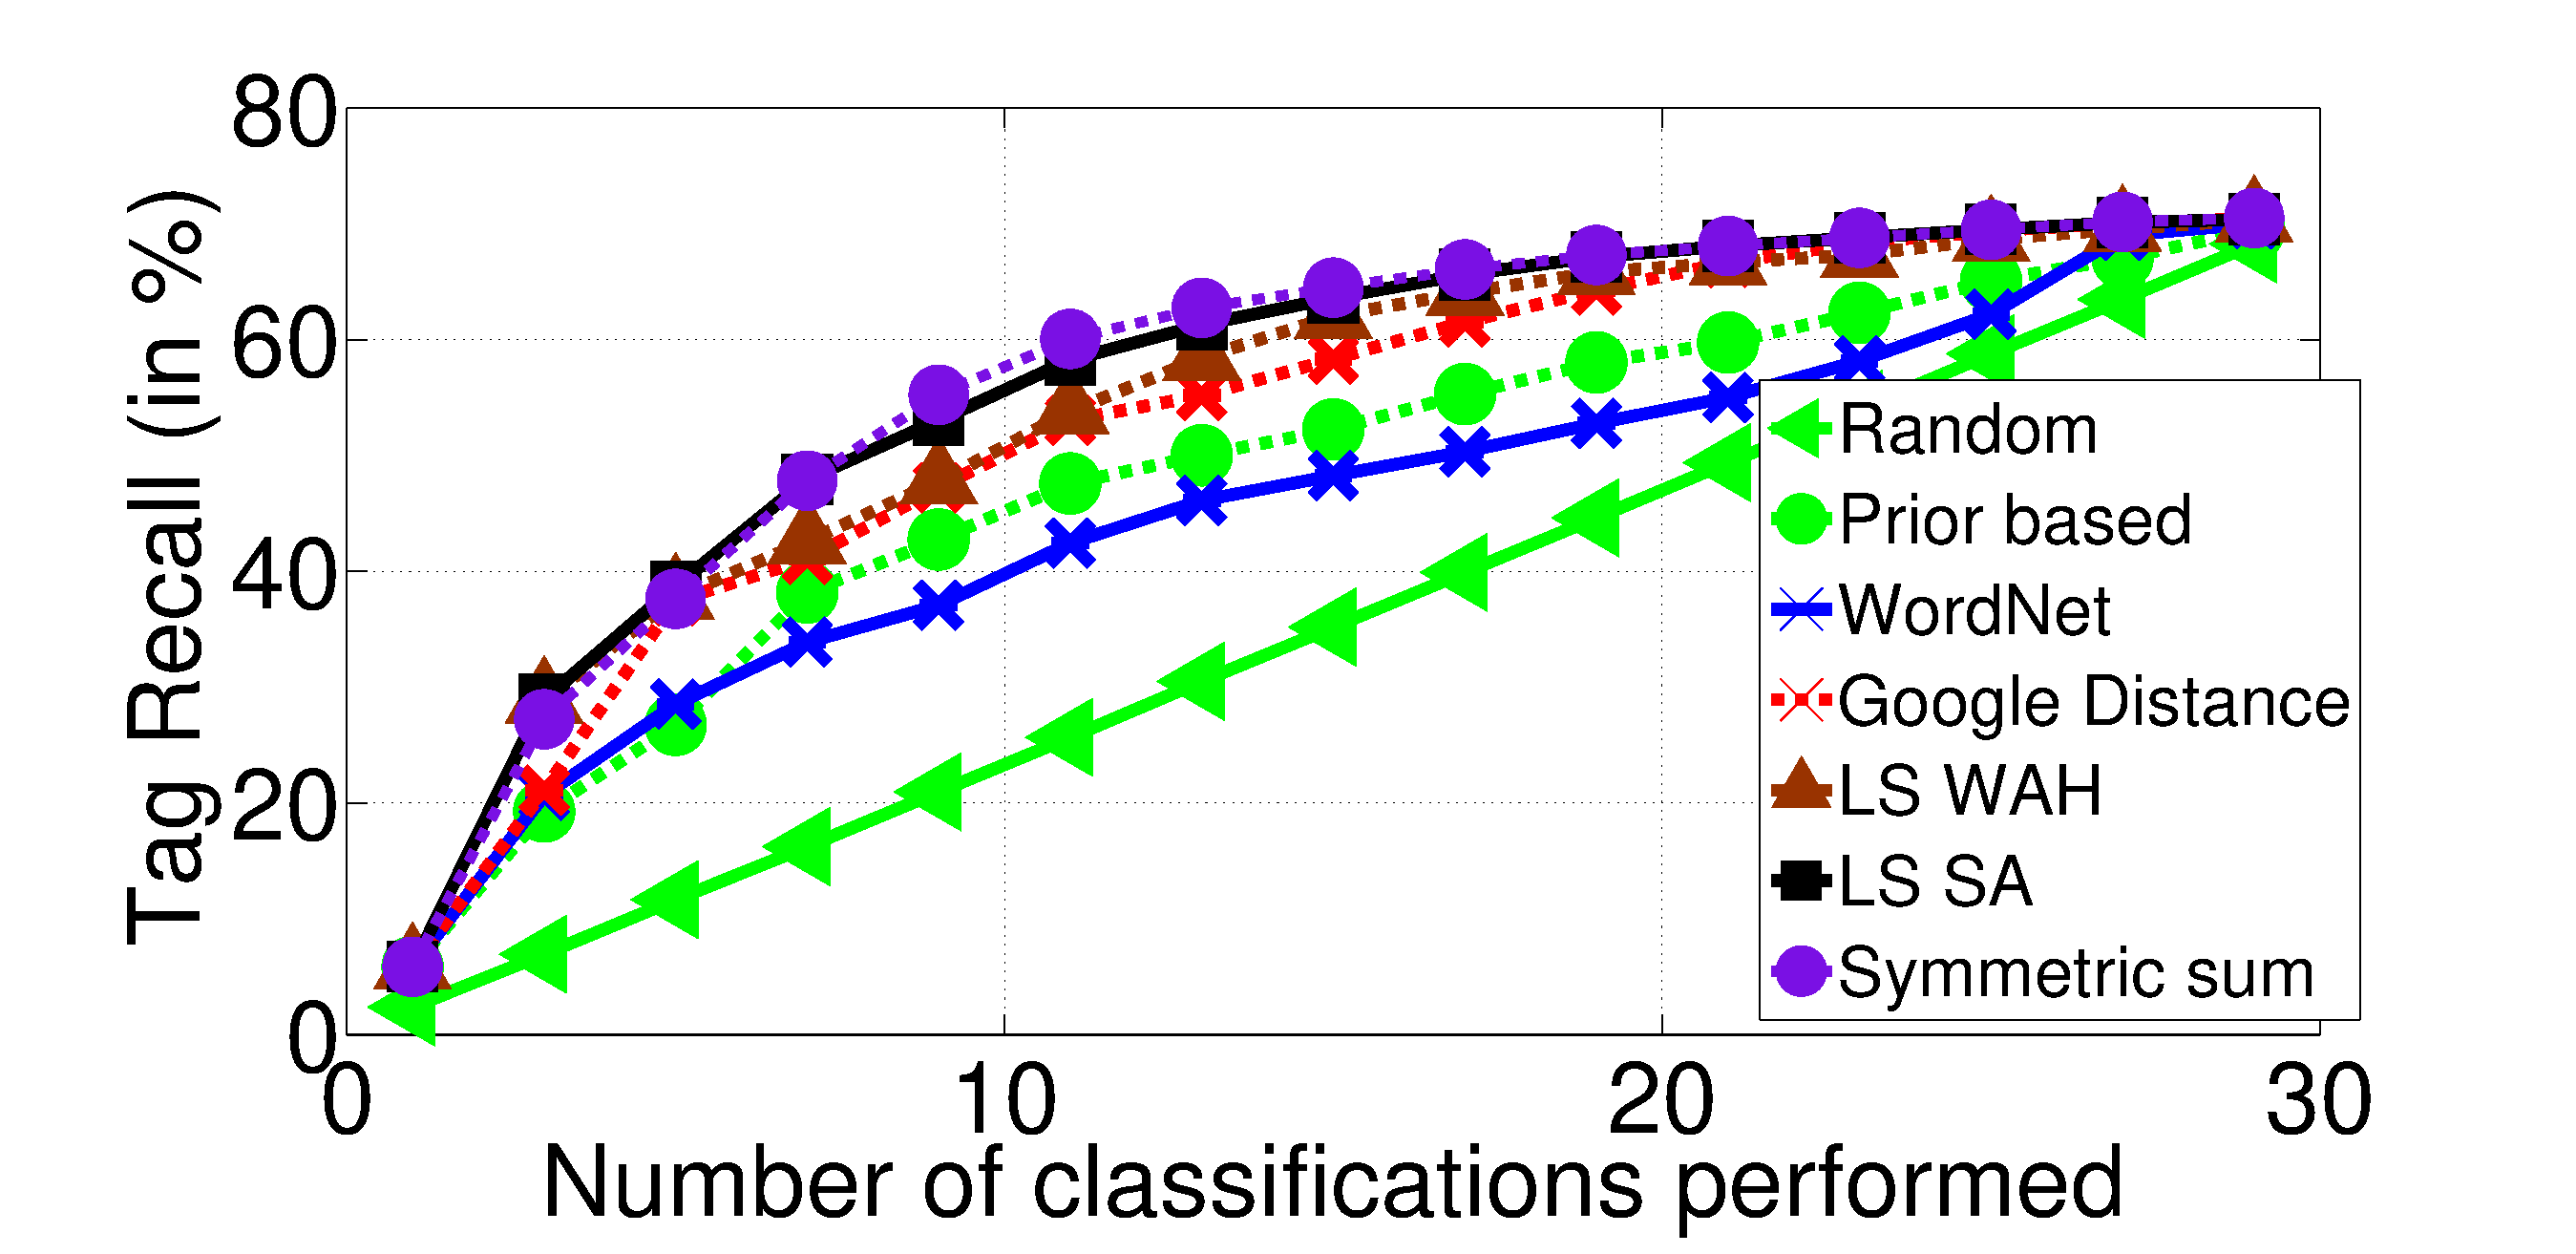
\includegraphics[width=0.65\linewidth]{TagTree/Rebuttal_FastTP_GWS}
\caption{\hl{Tag Recall obtained with respect to number of classifications performed for Stock images corpus. $\theta$ is chosen to  be 0.5. }}  
\label{fig:EfficientTagPredGraphGetty}
\end{figure}

\section{Robustness Analysis} \label{sec:Robustness}
We provide an analysis of the robustness of the proposed approach for constructing ontological tag trees. \hl{For the purpose of this section, we refer to the resource tag data using which the tag tree is constructed, as training data. The resource tag data over which the constructed tag tree is tested for evaluation purpose, is referred to as the test data}. \hl{As seen in Section {\ref{sec:Expts}}, the LS-SA method has consistently outperformed LS-WAH across different corpora and for both data-driven tasks}. Therefore, in this section we only study the robustness of the LS-SA method, i.e., the proposed local search based approach using Similarity Approximation based objective function (\ref{eq:ObjFnSimApprox}). In order to evaluate the constructed tag trees under various scenarios, we provide evaluation using tag prediction task as detailed in Section~\ref{subsec:TagPred}. \hl{Annotated image corpora are used for this purpose.} We study the robustness of proposed approach with respect to label noise, difference between training and test data, and the size of training data. These are discussed in detail below. 
\subsection{Robustness to Label Noise in Training Data}
\label{sec:RobustNoise}
\hl{As described in Section~{\ref{sec:Introduction}}, a vast majority of the user generated data available over the Internet has noisy labels (tags) associated with the resources}. We study the effect of different degrees of label noise on the tag tree constructed from such a noisy corpus. Fundamentally, we attempt to understand how robust the proposed tag tree construction approach is, to different degrees of label noise. We also attempt to answer questions such as - how much noise is too much for tag tree construction? 
\begin{figure}
%\epsfig{width=10cm,figure=VaryFWSorNoisewithGWSTPAccVary.eps}
%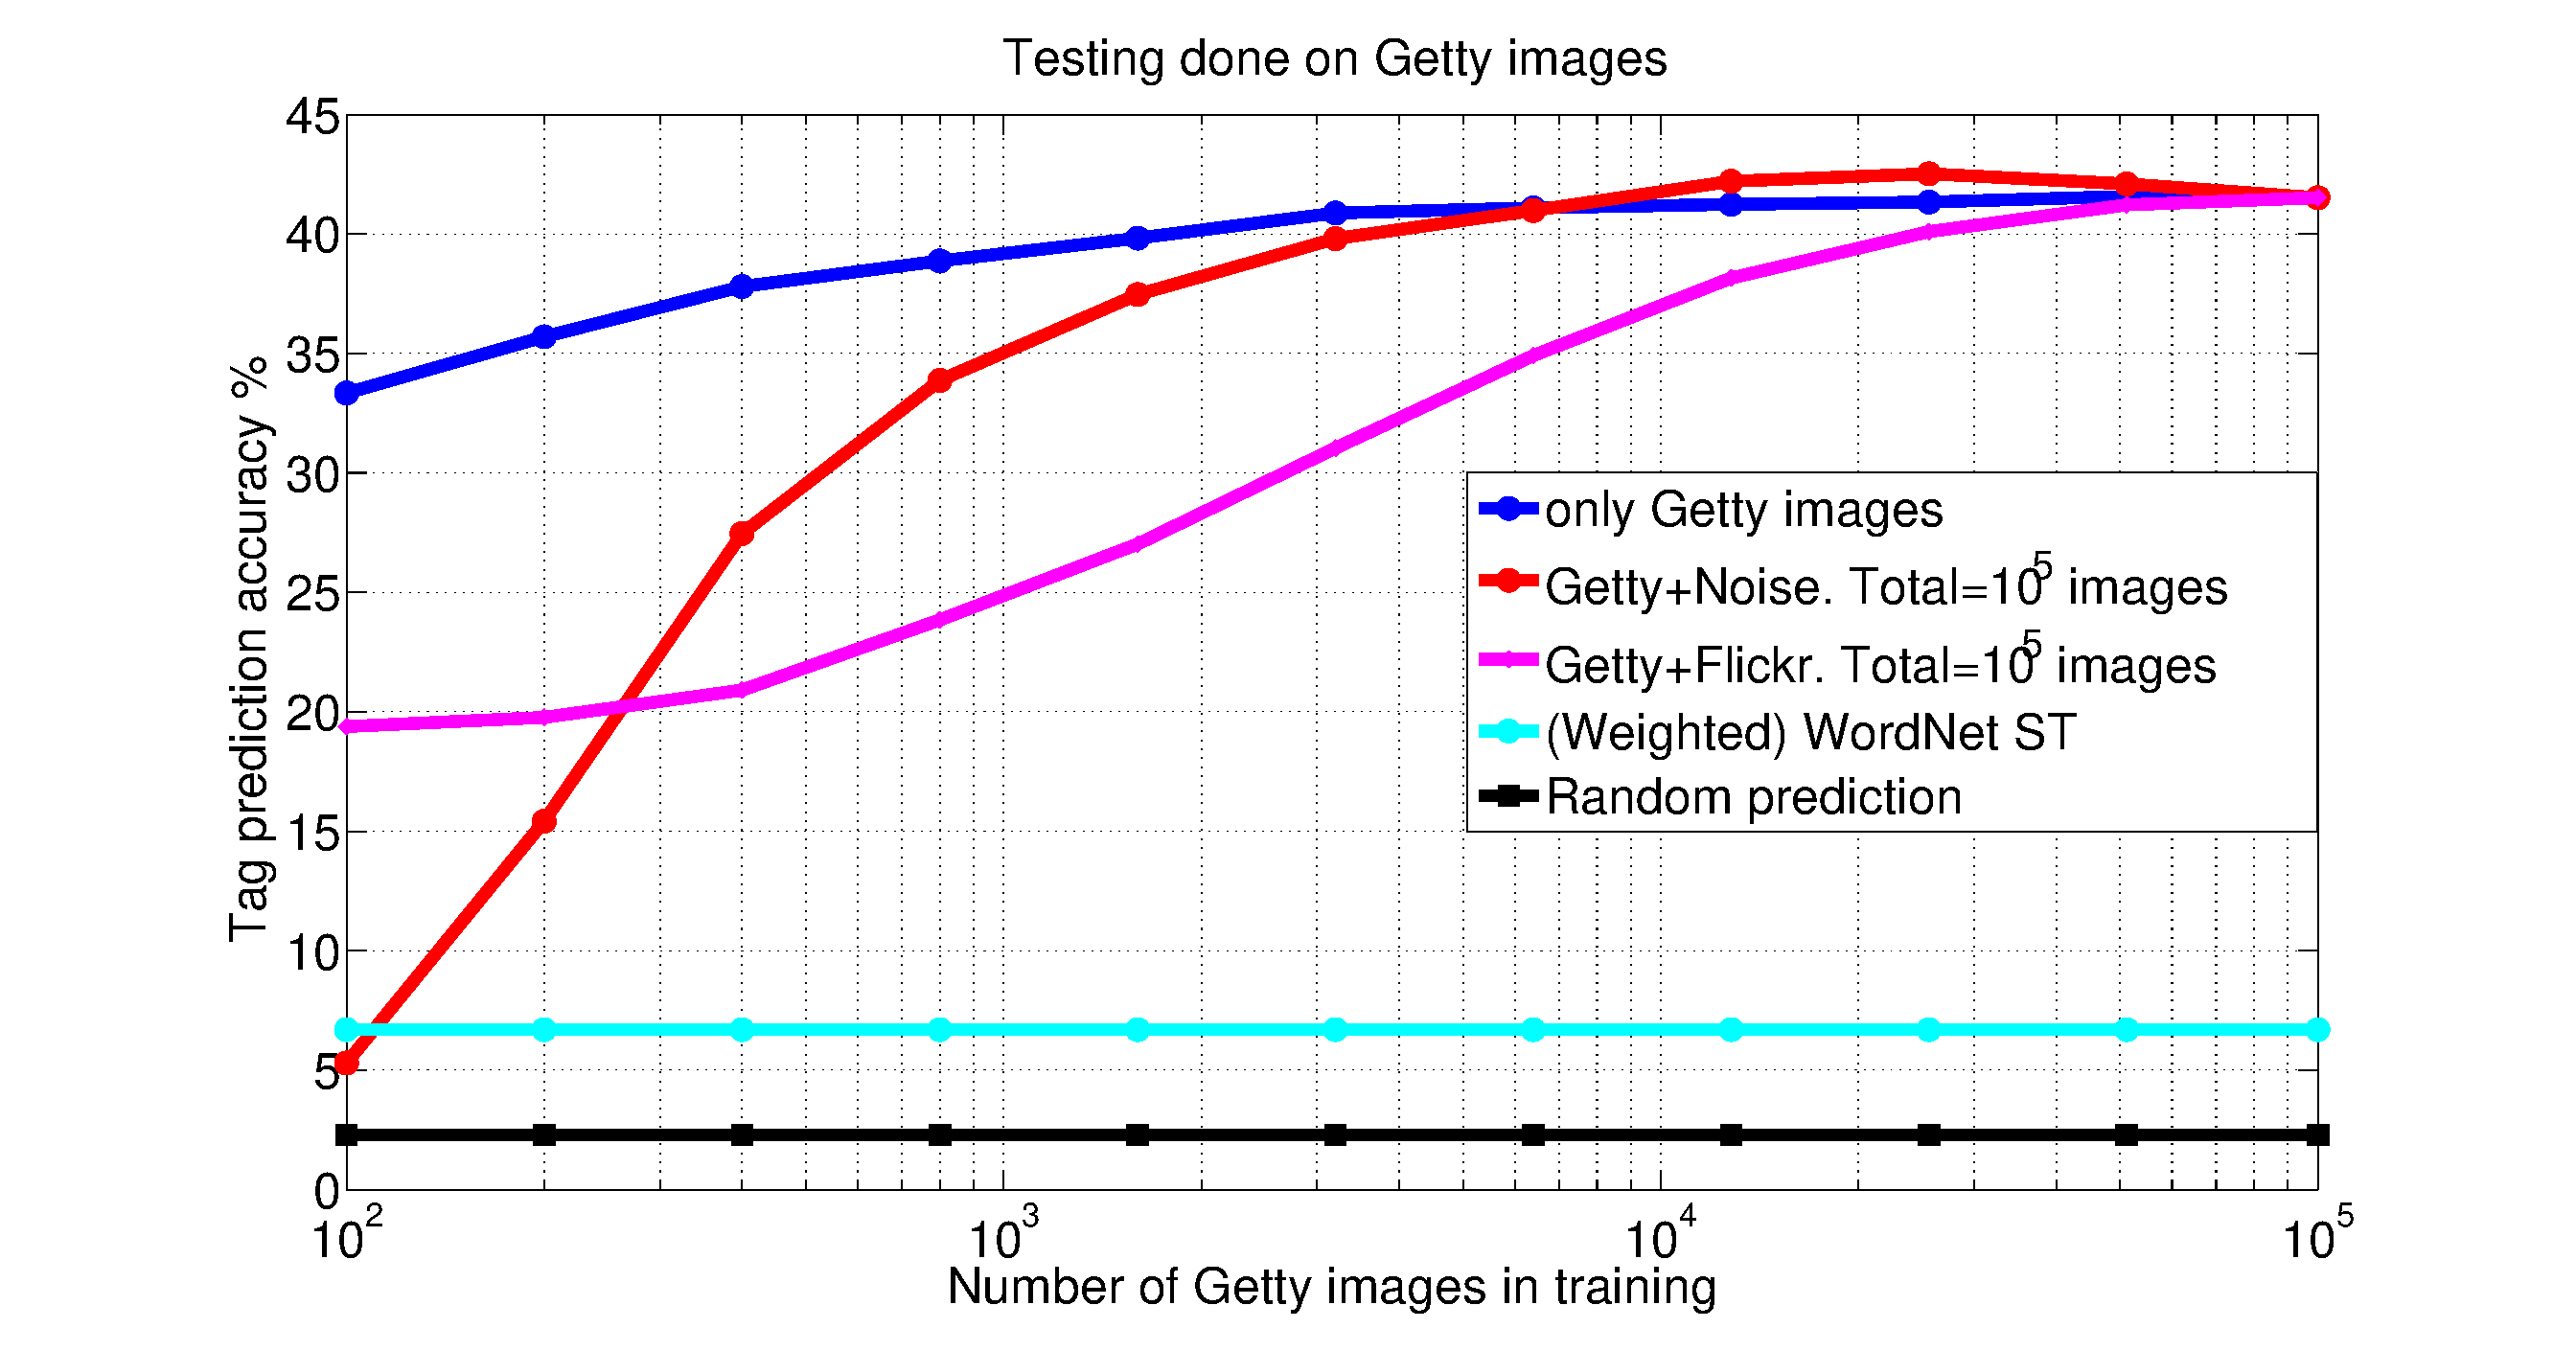
\includegraphics[width=\linewidth]{VaryFWSorNoisewithGWSTPAccVary}
\centering
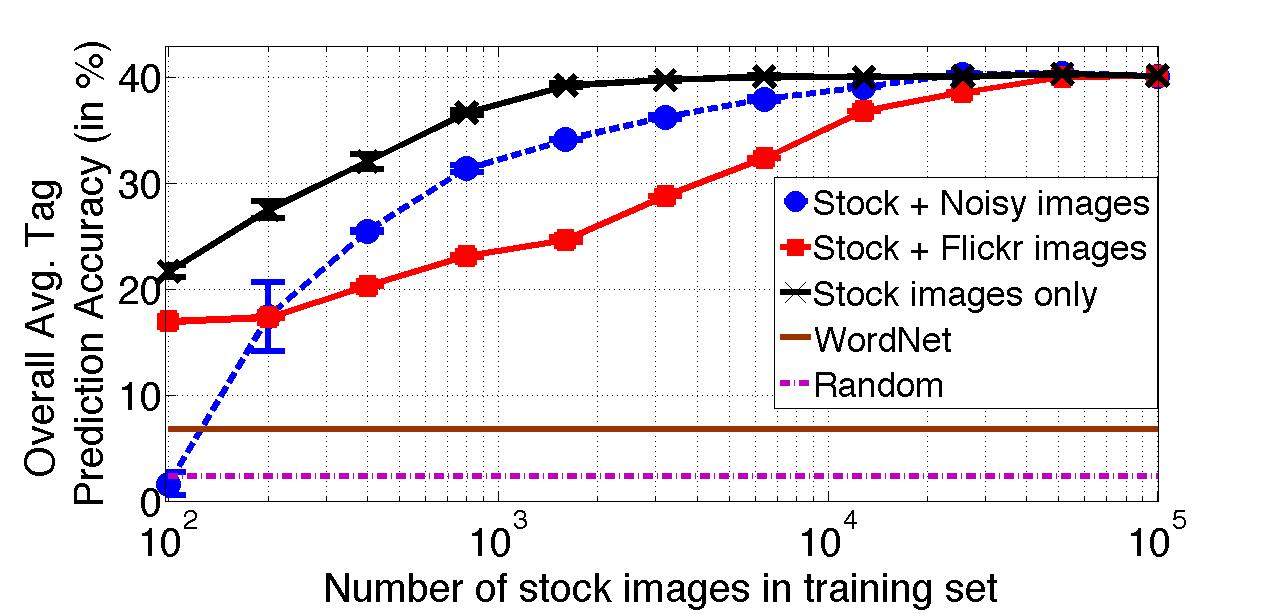
\includegraphics[width=0.65\linewidth]{TagTree/journal_RobustnessFig}
\caption{Overall Tag Prediction Score (in \%) obtained by proposed approach in Section~\ref{sec:TagPredUsingGraph}. The training set used to construct an ontological tag tree is formed by using certain number of stock images, with A) Flickr images, or B) noisy images, or C) none. Testing of the constructed tag tree is done on images of stock photos only. For comparison, the Overall Tag Prediction Accuracies for Random method, and WordNet method (as outlined in Section~\ref{sec:comparison}) are also provided. 
%A) 0.8\% (i.e., 800 in number) of stock images with the rest noisy images gives performance of 31.4\% as compared to 40.2\% when there are no noisy images while training. B) 0.8\% of stock images with the rest Flickr images in training set gives a performance of 23.1\%. C) Only 800 stock images with neither Flickr nor noisy images gives a performance of 36.7\%. 
} 
%\vspace{-5mm}
\label{fig:AddNoiseTrainingData}
\end{figure}

We work with stock image corpus since stock images are professionally curated and have little to no label noise, thus providing a better control on the amount of noise in the experimental data. We select top 150 tags (keywords) from this corpus and remove those that do not occur in Flickr or in WordNet. This gives a set $\mathcal{T}$  of 108 tags. Each stock image has on an average 3 tags amongst $\mathcal{T}$. A total of 100,000 stock images are used in training set and 50,000 stock images in the test set. In order to simulate varying degrees of label noise in training set, we replace stock images in the training data with artificially created images with noisy tags. The total number of training images (stock images and noisy images) is kept constant at 100,000. The artificially created noisy images are defined as images having exactly 3 randomly chosen tags from $\mathcal{T}$. The test set is not varied.  Fig. ~\ref{fig:AddNoiseTrainingData} shows the variation of Overall Tag Prediction Accuracy (\%) as defined in Section \ref{subsec:TagPred}, with number of images that were from stock images in the training set. It can be seen that even with 87.2\% noisy images in the training set, the performance of the constructed tag tree (39\%) is very close to the performance when there are no noisy images at all (40\%). Even when 99.2\% of the images in training set are noisy, the Overall Tag Prediction Accuracy is 31.4\%. An explanation for such performance even at high levels of noise is that the noisy images have uniformly random distribution of tags. The overall effect of adding noisy images to a corpus can be understood as adding certain intensity of white noise to the co-occurrence counts between tags. Unless the noise intensity dominates the corpus statistics, the relative order of pair-wise connections between tags remains fairly unchanged. In other words, since the noisy images have no strong biases towards specific tag-pairs, the performance of tag trees constructed using such a hybrid training set is not severely affected. 

\subsection{Robustness to Difference between Training and Test Data}
\label{sec:RobustDifference}
In several machine learning applications, the data over which a model is trained has certain amount of distributional difference as compared to the data over which it is tested. Looking at the construction of tag tree as model training, the degree to which a tag tree will be effective on a test set is a function of the difference between the test set and the training set using which the tag tree is constructed. Here we study how the performance of a tag tree varies for different degrees of difference between the training and the test sets. We utilize the same stock images corpus as used in Section~\ref{sec:RobustNoise}. In order to vary the difference between training and test sets, we replace varying number of stock images in training set with images from Flickr corpus (Section~\ref{sec:Datasets}). The total number of images (stock images and Flickr images) used for training of tag tree is kept constant at 100,000. Fig.~\ref{fig:AddNoiseTrainingData} shows the variation of Overall Tag Prediction Accuracy (\%) with number of images that were from stock images in the training set. It is interesting to note that for the same number of stock images, adding completely noisy images leads to better performance than adding Flickr images. For instance, for the case when 99.2\% of training images are from Flickr, performance of the constructed tag tree (23.1\%) is seen to be substantially worse than when 99.2\% of training images are noisy (31.4\%). The reason for this is that the tag distribution in Flickr corpus is not random, unlike in the case of noisy images. As a result, there are strong relationships between tags in Flickr corpus that are absent in stock image corpus. Constructing a tag tree on such a hybrid corpus attempts to capture corpus statistics of varying numbers of Flickr images and stock images, and in the process, is less effective at capturing the relationships that were present in the test data that has only stock images. 

\subsection{Size of Training Data}
\label{sec:RobustSize}
In this section, we study the effect of size of training set on construction of tag trees. Fig. ~\ref{fig:AddNoiseTrainingData} shows the variation of Overall Tag Prediction Accuracy (\%) with number of stock images in the training data. Here the size of training set is equal to the number of stock images in it and there are no Flickr images or noisy images. The performance of constructed tag tree improves with size of training data and almost saturates after certain number of training images. This is quite similar to the variation in performance of most machine learning models with the size of data over which they are trained. The performance of constructed tag tree from only 800 stock images is very close to the performance when 100,000 images are used. Even when only 100 stock images are used, the constructed tag tree performs much better than the tag trees using 100 stock images with 99900 Flickr or noisy images. Based on above, one can conclude that for the construction of ontological tag trees, it is better to use fewer training images than a larger set which is noisy or dissimilar to the test set.  
\comment{
\begin{figure}[htbp]
\centering
\begin{tabular}{p{2.2cm} p{2.2cm} p{3cm}}
\centering
\epsfig{width=2cm,height=2.8cm,figure=TagTree/figures/3569597369_690c84559a.eps} & %32965350@N00
\epsfig{width=2cm,height=2.8cm,figure=TagTree/figures/183307784_ca9034cc51.eps} & %85598619@N00
\epsfig{width=2.8cm,height=2cm,figure=TagTree/figures/180824073_fc5f017f46.eps}\\ %22768390@N00
(a){\bf holiday, island}, travel, vacation, water&
(b){\bf england, street}, building, london,uk&
(c){\bf germany, travel}, deutschland, europe, summer\\
\end{tabular}
\caption{A few examples where the local search based refinement was able to predict two of the three tags correctly, given two original tags (shown in bold). Tag prediction based on WordNet did not result in correct prediction for these examples. The Flickr owner and photo ids of these images are (32965350@N00,3569597369), (85598619@N00,183307784), (22768390@N00,180824073) respectively.}
\label{fig:examples}
\end{figure}
}
\begin{figure*}
        \centering
	\captionsetup{justification=raggedright,
	singlelinecheck=false
	}
        \begin{subfigure}[b]{0.16\textwidth}
                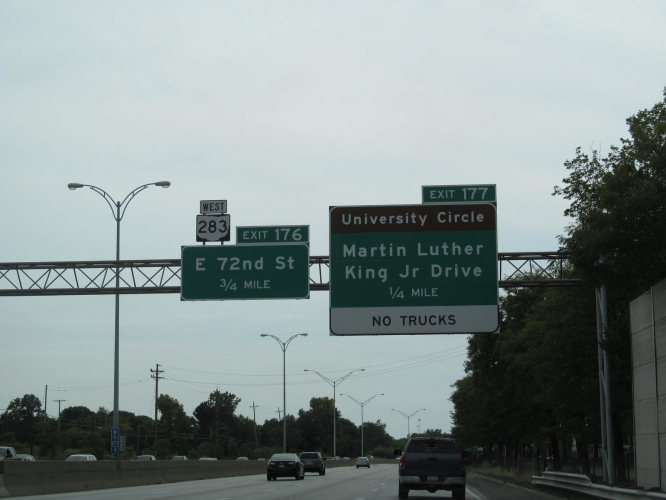
\includegraphics[width=0.8\textwidth]{TagTree/Flickrimg/777b9480-f735-3d7a-aa91-dba84cea8bf2.jpeg} 
                \caption{\textbf{Seen}: highway, road \\ \textbf{Unseen}: route, shield, sign }
                \label{fig:posex1}
        \end{subfigure}%
	\; \vline
        \; %add desired spacing between images, e. g. ~, \quad, \qquad etc.
          %(or a blank line to force the subfigure onto a new line)
        \begin{subfigure}[b]{0.17\textwidth}
                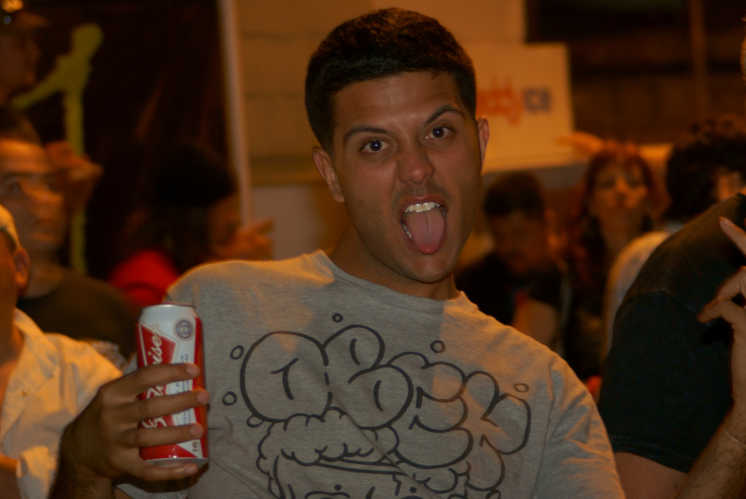
\includegraphics[width=0.8\textwidth]{TagTree/Flickrimg/e3bb5574-1a09-32cf-9f22-1a9eb81af7c2.jpeg}
                \caption{\textbf{Seen}: austin, \\ band \\ \textbf{Unseen}: music, texas, tx }
                \label{fig:posex2}
        \end{subfigure}%
	\; \vline
        \; %add desired spacing between images, e. g. ~, \quad, \qquad etc.
          %(or a blank line to force the subfigure onto a new line)
        \begin{subfigure}[b]{0.17\textwidth}
                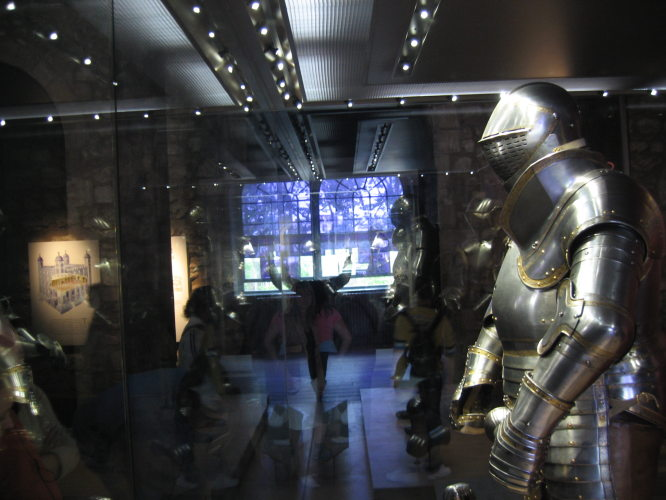
\includegraphics[width=0.8\textwidth]{TagTree/Flickrimg/7c52f0a2-78ae-3b9b-9dd0-f131124750f5.jpeg}
                \caption{\textbf{Seen}: england, europe \\ \textbf{Unseen}: london, travel, uk }
                \label{fig:posex3}
        \end{subfigure}%
	\; \vline
        \; %add desired spacing between images, e. g. ~, \quad, \qquad etc.
          %(or a blank line to force the subfigure onto a new line)
        \begin{subfigure}[b]{0.16\textwidth}
                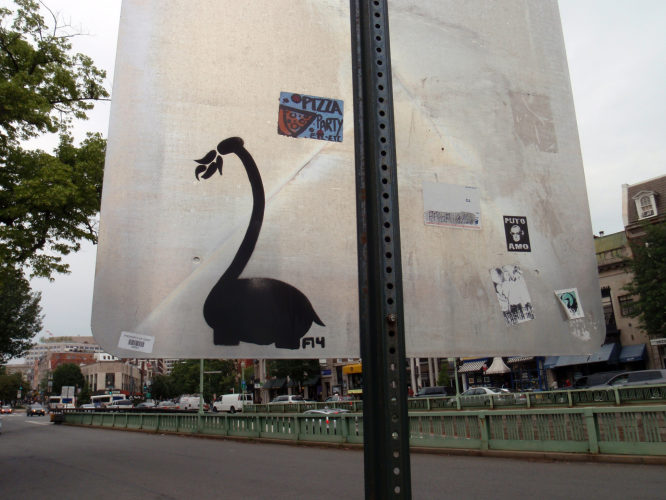
\includegraphics[width=0.8\textwidth]{TagTree/Flickrimg/b03623e7-e6cf-3e96-97cc-a7117c776614.jpeg}
                \caption{\textbf{Seen}: art, dc \\ \textbf{Unseen}: graffiti, street, washington }
                \label{fig:posex4}
        \end{subfigure}%
	\; \vline
        \; %add desired spacing between images, e. g. ~, \quad, \qquad etc.
          %(or a blank line to force the subfigure onto a new line)
        \begin{subfigure}[b]{0.17\textwidth}
                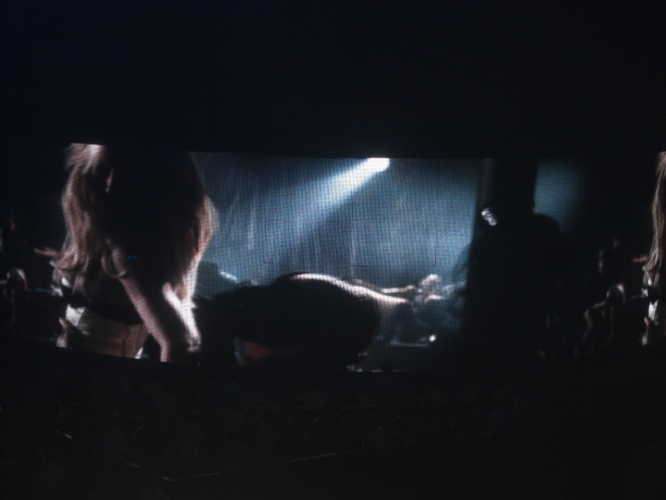
\includegraphics[width=0.8\textwidth]{TagTree/Flickrimg/8efd5e1c-6d83-37af-91a2-1484a9d823b3.jpeg}
                \caption{\textbf{Seen}: concert, england\\ \textbf{Unseen}: london, music, uk }
                \label{fig:posex5}
        \end{subfigure}
        \caption{Example images where LS-SA method gave 100\% tag prediction accuracy when the first two tags were seen and the next three were unseen and predicted. The Flickr owner and photo ids of these images are (dougtone@7975042008) ,  (elchupacabra@7023118527) , (jeffwilcox@159730021) , (daquellamanera@4678084101) , (martinrp@3832812191)  respectively. } \label{fig:positiveExs}
\end{figure*}

\begin{figure*}
        \centering
	\captionsetup{justification=raggedright,
	singlelinecheck=false
	}
        \begin{subfigure}[b]{0.16\textwidth}
                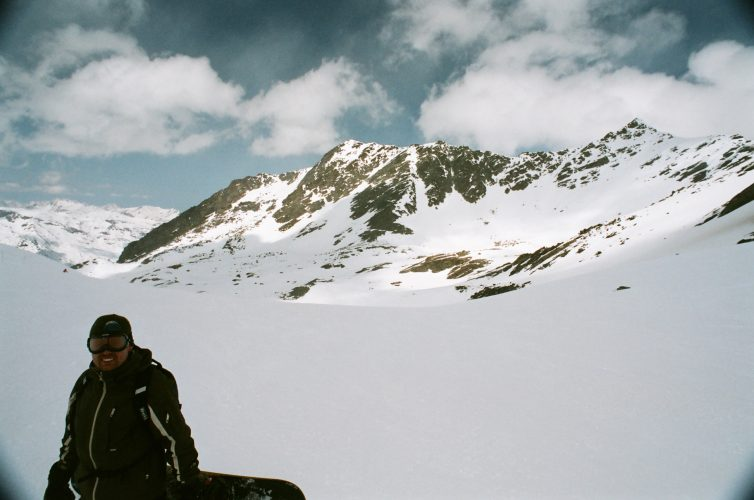
\includegraphics[width=\textwidth]{TagTree/Flickrimg/7a6b7ae7-7afb-3f90-92df-e67c0bd22a8a.jpeg}
                \caption{\textbf{Seen}: film, france \\ \textbf{Unseen}: holiday, \\ sky, snow \\ \textbf{Predicted}: paris, europe, bw }
                \label{fig:negex1}
        \end{subfigure}%
	\; \vline
        \; %add desired spacing between images, e. g. ~, \quad, \qquad etc.
          %(or a blank line to force the subfigure onto a new line)
        \begin{subfigure}[b]{0.17\textwidth}
                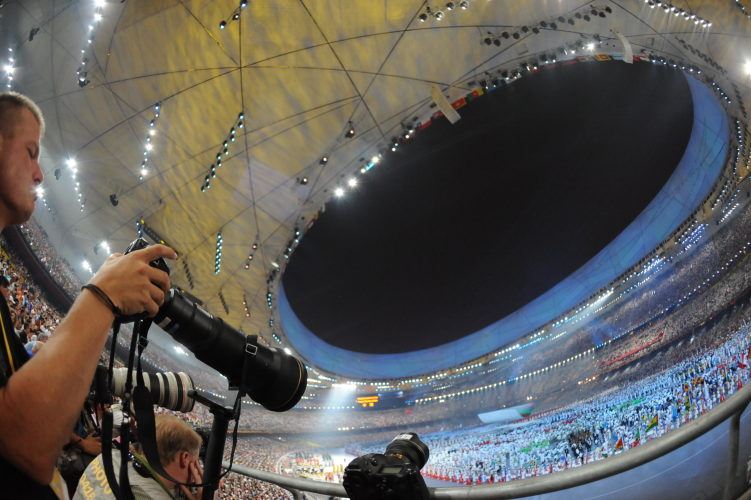
\includegraphics[width=0.8\textwidth]{TagTree/Flickrimg/ec4436dd-57b3-36af-94f6-64cf05294886.jpeg}
                \caption{\textbf{Seen}: china, family \\ \textbf{Unseen}: live, summer, \\ usa  \\ \textbf{Predicted}: photography, christmas, photo }
                \label{fig:negex2}
        \end{subfigure}%
	\; \vline
        \; %add desired spacing between images, e. g. ~, \quad, \qquad etc.
          %(or a blank line to force the subfigure onto a new line)
        \begin{subfigure}[b]{0.16\textwidth}
                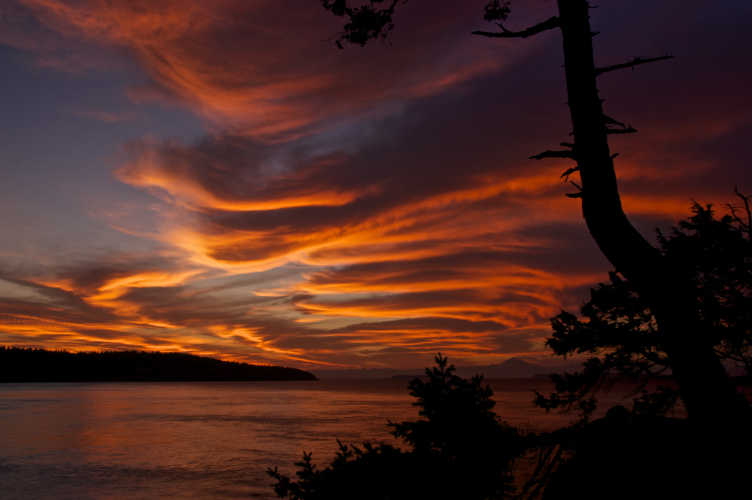
\includegraphics[width=0.8\textwidth]{TagTree/Flickrimg/bf51a02f-baa1-3861-a300-12b5f654c456.jpeg}
                \caption{\textbf{Seen}: canada, \\ ocean \\ \textbf{Unseen}: red, sky, sunset \\ \textbf{Predicted}: sea, beach, water }
                \label{fig:negex3}
        \end{subfigure}%
	\; \vline
        \; %add desired spacing between images, e. g. ~, \quad, \qquad etc.
          %(or a blank line to force the subfigure onto a new line)
        \begin{subfigure}[b]{0.17\textwidth}
                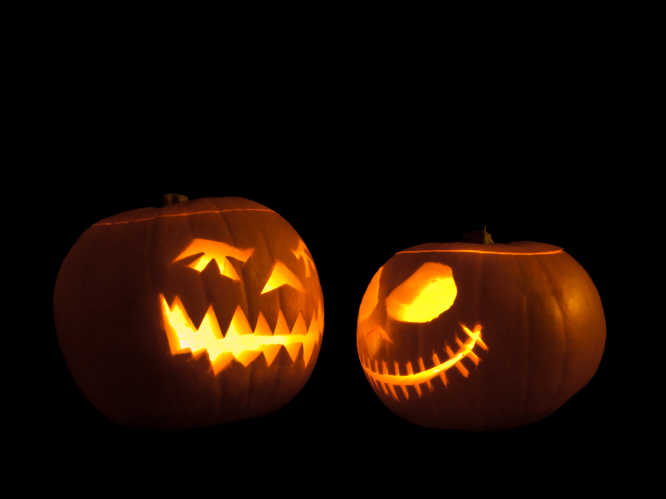
\includegraphics[width=0.8\textwidth]{TagTree/Flickrimg/b339e52a-b87e-347a-8ba8-12502fc11443.jpeg}
                \caption{\textbf{Seen}: autumn, \\ black\\ \textbf{Unseen}: light, macro, night \\ \textbf{Predicted}: white, nature, bw }
                \label{fig:negex4}
        \end{subfigure}%
	\; \vline
        \; %add desired spacing between images, e. g. ~, \quad, \qquad etc.
          %(or a blank line to force the subfigure onto a new line)
        \begin{subfigure}[b]{0.18\textwidth}
                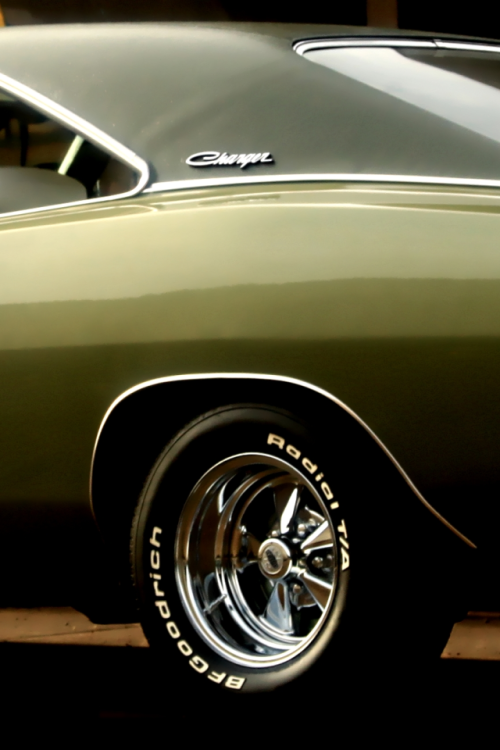
\includegraphics[width=0.45\textwidth]{TagTree/Flickrimg/acf2533e-69ac-3e2e-8eab-e024ca9682fd.jpeg}
                \caption{\textbf{Seen}: car, green \\ \textbf{Unseen}: photo, washington, white \\ \textbf{Predicted}: red, spring, nature }
                \label{fig:negex5}
        \end{subfigure}
        \caption{Example images where LS-SA method gave 0\% tag prediction accuracy when the first two tags were seen and the next three were unseen and predicted. Also provided are the tags that were predicted by the LS-SA method. The Flickr owner and photo ids of these images
are (king-edward@4061393892) , (familymwr@4928996212) , (alejandroerickson@7730525250) , (wwarby@5145467790) ,  (1968-dodge-charger@5507716438)  respectively. \textbf{Seen: ($\mathcal{T}_{i,Seen}$); Unseen: ($\mathcal{T}_i \setminus  \mathcal{T}_{i,Seen}$); Predicted: ($\mathbb{P}_i$)} as per Section~\ref{subsec:TagPred}. }  \label{fig:negativeExs}
\end{figure*}
